\nonstopmode
%DIF LATEXDIFF DIFFERENCE FILE
%DIF DEL ../../2nd circ/ANA-TRIG-2021-01-PAPER/ANA-TRIG-2021-01-PAPER.tex   Thu Nov 14 15:26:24 2024
%DIF ADD ANA-TRIG-2021-01-PAPER.tex                                         Thu Nov 14 15:26:24 2024

\RequirePackage{silence}
\WarningsOff[typearea]


%-------------------------------------------------------------------------------
% This file provides a skeleton ATLAS paper.
%-------------------------------------------------------------------------------
% \pdfoutput=1
% The \pdfoutput command is needed by arXiv/JHEP/JINST to ensure use of pdflatex.
% It should be included in the first 5 lines of the file.
\pdfinclusioncopyfonts=1
% This command may be needed in order to get \ell in PDF plots to appear. Found in
% https://tex.stackexchange.com/questions/322010/pdflatex-glyph-undefined-symbols-disappear-from-included-pdf
%-------------------------------------------------------------------------------
% Specify where ATLAS LaTeX style files can be found.
\RequirePackage{latex/atlaslatexpath}
% Comment out the above line if the files are in a central location, e.g. $HOME/texmf.
%-------------------------------------------------------------------------------
\documentclass[PAPER, atlasdraft=true, UKenglish, coverpage]{atlasdoc}
% The language of the document must be set: usually UKenglish or USenglish.
% british and american also work!
% Commonly used options:
%  atlasdraft=true|false This document is an ATLAS draft.
%  coverpage             Create ATLAS draft cover page for collaboration circulation.
%                        See atlas-draft-cover.tex for a list of variables that should be defined.
%  cernpreprint          Create front page for a CERN preprint.
%                        See atlas-preprint-cover.tex for a list of variables that should be defined.
%  NOTE                  The document is an ATLAS note (draft).
%  PAPER                 The document is an ATLAS paper (draft).
%  CONF                  The document is a CONF note (draft).
%  PUB                   The document is a PUB note (draft).
%  BOOK                  The document is of book form, like an LOI or TDR (draft).
%  paper=a4|letter       Set paper size to A4 (default) or letter.


\usepackage[utf8]{inputenc}
\usepackage{textcomp} % solve issues of missing unicode chars
\usepackage{caption}
%\usepackage{amsmath,amssymb}
%\usepackage[makeroom]{cancel} % For the cancel symbol
\usepackage{graphicx}
\usepackage{rotating} % Para rodar as figuras e tabelas
\usepackage{pdflscape} % Para colocar paginas na horizontal no pdf
\usepackage{array,booktabs}
\usepackage{multirow} % Tabelas com celulas agrupadas
\usepackage{placeins} % mais floats (figuras tabelas etc)!
%\usepackage{import} % To access created latex images in different folders
\usepackage{enumerate} % To have access to special enumerations
\usepackage{geometry} % Make rotations be in landscape
\usepackage{scalerel} % scale
%\usepackage{stackengine} % stackon stackunder
%\usepackage{tablefootnote} % Footnotes inside tables
\usepackage{nicefrac} % for fractions
%\usepackage{algorithm}
%\usepackage{algorithmic}
%\usepackage[dvipsnames]{xcolor}
\usepackage{colortbl}
\usepackage{tabulary}
\usepackage[linesnumbered,ruled,vlined]{algorithm2e}
\usepackage{multirow}
\usepackage{comment}
\usepackage{subcaption}



%-------------------------------------------------------------------------------
% Extra packages:
\usepackage{atlaspackage}
% Commonly used options:
%  subfigure|subfig|subcaption  to use one of these packages for figures in figures.
%  minimal               Minimal set of packages.
%  default               Standard set of packages.
%  full                  Full set of packages.
%-------------------------------------------------------------------------------

% Style file with biblatex options for ATLAS documents.
\usepackage{atlasbiblatex}

% Useful macros
\usepackage{atlasphysics}
% See doc/atlas_physics.pdf for a list of the defined symbols.
% Default options are:
%   true:  journal, misc, particle, unit, xref
%   false: BSM, hepparticle, hepprocess, hion, jetetmiss, math, process,
%          other, snippets
% See the package for details on the options.

% Macro to add to-do notes (for several authors). Uses the todonotes package.
% \ATLnote{JS}{Jane}{green!20}{green!50!black!60}
% add macros \JSnote and \JSinote for notes in the margin and inline.
% The first colour is for the body and the second for the border of the note.
% Set output=false in order not to print out the notes.
% Set shift=false to avoid adjustment of margins.
% This package should not be used in the final version of the paper.
\ifthenelse{\boolean{AtlasDraft}}{\usepackage[output=true, shift=true]{atlastodo}}{}

% Files with references for use with biblatex.
% Note that biber gives an error if it finds empty bib files.
\addbibresource{ANA-TRIG-2021-01-PAPER.bib}
\addbibresource{bib/ATLAS.bib}
\addbibresource{bib/CMS.bib}
\addbibresource{bib/ConfNotes.bib}
\addbibresource{bib/PubNotes.bib}

% Paths for figures - do not forget the / at the end of the directory name.
\graphicspath{{logos/}{figures/}}

% Add your own definitions here (file ANA-TRIG-2021-01-PAPER-defs.sty).
\usepackage{ANA-TRIG-2021-01-PAPER-defs}

%-------------------------------------------------------------------------------
% Generic document information.
%-------------------------------------------------------------------------------

% Title, abstract and document.
%-------------------------------------------------------------------------------
% This file contains the title, author and abstract.
% It also contains all relevant document numbers used by the different cover pages.
%-------------------------------------------------------------------------------

% Title
\AtlasTitle{Implementation and \DIFdelbegin \DIFdel{Performance }\DIFdelend \DIFaddbegin \DIFadd{performance }\DIFaddend of the Neural-Ringer \DIFdelbegin \DIFdel{Algorithm Selecting Electrons at the High Level Trigger }\DIFdelend \DIFaddbegin \DIFadd{electron selection algorithm in the high-level trigger }\DIFaddend of the ATLAS \DIFdelbegin \DIFdel{Experiment}\DIFdelend \DIFaddbegin \DIFadd{experiment}\DIFaddend }

% Draft version:
% Should be 1.0 for the first circulation, and 2.0 for the second circulation.
% If given, adds draft version on front page, a 'DRAFT' box on top of every other page, 
% and line numbers.
% Comment or remove in the final version.
\AtlasVersion{2}

% Abstract - % directly after { is important for correct indentation
\AtlasAbstract{%

Electron trigger identification is a crucial input to many ATLAS physics analysis. To cope with the increase \DIFdelbegin \DIFdel{of }\DIFdelend \DIFaddbegin \DIFadd{in }\DIFaddend peak LHC luminosity from 2017 to 2018\DIFdelbegin \DIFdel{that pushed }\DIFdelend \DIFaddbegin \DIFadd{, which raised }\DIFaddend the number of \DIFdelbegin \DIFdel{proton-proton }\DIFdelend \DIFaddbegin \DIFadd{proton--proton }\DIFaddend interactions per beam-crossing to about 60, trigger algorithms were optimized to keep the background trigger rates low while retaining \DIFdelbegin \DIFdel{a }\DIFdelend high efficiency for physics analyses. 
In the second half of 2017, the Neural-Ringer algorithm, \DIFdelbegin \DIFdel{which is }\DIFdelend \DIFaddbegin \DIFadd{based on }\DIFaddend a set of \DIFdelbegin \DIFdel{Multi-Layer Perception (MLP) }\DIFdelend \DIFaddbegin \DIFadd{multi-layer perceptron }\DIFaddend models, replaced the cut-based strategy \DIFaddbegin \DIFadd{used }\DIFaddend in the FastCalo decision step \DIFaddbegin \DIFadd{in the high-level trigger }\DIFaddend and became the baseline algorithm for triggering events containing electrons \DIFaddbegin \DIFadd{with transverse energy }\DIFaddend above 15\DIFdelbegin \DIFdel{GeV in the High Level Trigger (HLT), }\DIFdelend \DIFaddbegin \DIFadd{~GeV. This was done }\DIFaddend as part of the ATLAS online system \DIFdelbegin \DIFdel{CPU }\DIFdelend \DIFaddbegin \DIFadd{CPU-time }\DIFaddend reduction campaign.
It was the first time a \DIFdelbegin \DIFdel{neural network }\DIFdelend \DIFaddbegin \DIFadd{neural-network }\DIFaddend method was employed as a baseline \DIFdelbegin \DIFdel{selection }\DIFdelend algorithm for event selection in the ATLAS trigger system\DIFdelbegin \DIFdel{which results in a higher background early rejection strategy, }\DIFdelend \DIFaddbegin \DIFadd{,
and resulted in the early rejection of }\DIFaddend at least 13 times \DIFdelbegin \DIFdel{with respect to }\DIFdelend \DIFaddbegin \DIFadd{more background than }\DIFaddend the cut-based \DIFdelbegin \DIFdel{, while maintaining electron }\DIFdelend \DIFaddbegin \DIFadd{strategy, while leaving the electron selection }\DIFaddend efficiency nearly unchanged.




}

% Author - this does not work with revtex (add it after \begin{document})
% This has to be commented out for TDR etc.
% For PUB notes, add package authblk and use \thanks if an ACE/STA should be added.
% See Section 4.2 of ATLAS LaTeX guide and latex/atlascontribute.sty for more details.
% \author{The ATLAS Collaboration}

% ATLAS reference code, to help ATLAS members to locate the paper
\AtlasRefCode{TRIG-2021-01}

% CERN preprint number
% \PreprintIdNumber{CERN-EP-2024-XX}

% ATLAS date - arXiv submission; usually filled in by the Physics Office
% \AtlasDate{\today}

% ATLAS heading - heading at top of title page. Set for TDR etc.
% \AtlasHeading{ATLAS ABC TDR}

% Keywords - some journals want keywords on the title page.
% You have to pass the option keywords=true to atlasdoc for this to be effective.
% \AtlasKeywords{keywords}

% Copyright - use if something other than the default copyright is required.
% You have to pass the option copyright=true to atlasdoc for this to be effective.
% \AtlasCopyright{\the\year \ CERN for the benefit of the ATLAS Collaboration.\newline
%   Reproduction of this article or parts of it is allowed as specified in the CC-BY-4.0 license.}

% arXiv identifier
% \arXivId{21XX.YYYY}

% HepData record
% \HepDataRecord{ZZZZZZZZ}

% Submission journal and final reference
\AtlasJournal{JINST}
%\AtlasJournal{IEEE transactions on nuclear science}
% \AtlasJournalRef{\PLB 789 (2023) 123}
% \AtlasDOI{}

% Some papers/public notes have a special author list.
% If a special author list should be indicated via a link use the following code:
% Include the two lines below if you do not use atlasstyle:
% \usepackage[marginal,hang]{footmisc}
% \setlength{\footnotemargin}{0.5em}
% Use the following lines in all cases:
% \usepackage{authblk}
% \author{The ATLAS Collaboration%
% \thanks{The full author list can be found at:\newline
%   \url{https://atlas.web.cern.ch/Atlas/PUBNOTES/ATL-PHYS-PUB-2024-XXX/authorlist.pdf}}
% }
% You may need the following lines if the affiliation number does not appear as a superscript
% when you are using authblk.
% \makeatletter
% \renewcommand\AB@authnote[1]{{\normalfont\textsuperscript{#1}}}
% \renewcommand\AB@affilnote[1]{{\normalfont\textsuperscript{#1}}}
% \makeatother

%-------------------------------------------------------------------------------
% The following information is needed for the cover page. The commands are defined
% if you use the coverpage option in atlasdoc or use the atlascover package.
% They are also defined if you include the atlasmetadefs package.
%-------------------------------------------------------------------------------

% List of supporting notes  (leave as null \AtlasCoverSupportingNote{} if you want to skip this option)
\AtlasCoverSupportingNote{Support Note}{https://cds.cern.ch/record/2777971/}
%
% OR (the 2nd option is deprecated, especially for CONF and PUB notes)
%
% Supporting material TWiki page  (leave as null \AtlasCoverTwikiURL{} if you want to skip this option)
% \AtlasCoverTwikiURL{https://twiki.cern.ch/twiki/bin/view/Atlas/WebHome}

% Comment deadline
\AtlasCoverCommentsDeadline{21 November 2024}

% Analysis team members - contact editors should no longer be specified
% as there is a generic email list name for the editors
\AtlasCoverAnalysisTeam{Jose Seixas, Denis Oliveira Damazio, Chris Meyer, Werner Spolidoro Freund, Joao Victor Da Fonseca Pinto, Micael Verissimo De Araujo}

% Editorial Board Members - indicate the Chair by a (chair) after his/her name
% Give either all members at once (then they appear on one line), or separately
\AtlasCoverEdBoardMember{Bertrand, Laforge (Paris LPNHE) }
\AtlasCoverEdBoardMember{Fernando, Monticelli (La Plata) (chair)}
% \AtlasCoverEdBoardMember{EdBoard~Chair~(chair)}
% \AtlasCoverEdBoardMember{EB~Member~1}
% \AtlasCoverEdBoardMember{EB~Member~2}
% \AtlasCoverEdBoardMember{EB~Member~3}



% Analysis team egroup
\AtlasCoverEgroupAnalysisTeam{atlas-TRIG-2021-01-analysis-team@cern.ch}

% EdBoard and conveners egroup
\AtlasCoverEgroupEdBoard{atlas-TRIG-2021-01-edboard-conveners@cern.ch}

% Author and title for the PDF file.
\hypersetup{pdftitle={ATLAS document},pdfauthor={The ATLAS Collaboration}}

%-------------------------------------------------------------------------------
% Content
%-------------------------------------------------------------------------------



%-------------------------------------------------------------------------------
\setcounter{secnumdepth}{4}
\setcounter{tocdepth}{4}
%-------------------------------------------------------------------------------
% Get old font commands back
%-------------------------------------------------------------------------------
\makeatletter
%\DeclareOldFontCommand{\rm}{\normalfont\rmfamily}{\mathrm}
%\DeclareOldFontCommand{\sf}{\normalfont\sffamily}{\mathsf}
%\DeclareOldFontCommand{\tt}{\normalfont\ttfamily}{\mathtt}
%\DeclareOldFontCommand{\bf}{\normalfont\bfseries}{\mathbf}
\DeclareOldFontCommand{\it}{\normalfont\itshape}{\mathit}
%\DeclareOldFontCommand{\sl}{\normalfont\slshape}{\@nomath\sl}
%\DeclareOldFontCommand{\sc}{\normalfont\scshape}{\@nomath\sc}
\makeatother
%DIF PREAMBLE EXTENSION ADDED BY LATEXDIFF
%DIF UNDERLINE PREAMBLE %DIF PREAMBLE
\RequirePackage[normalem]{ulem} %DIF PREAMBLE
\RequirePackage{color}\definecolor{RED}{rgb}{1,0,0}\definecolor{BLUE}{rgb}{0,0,1} %DIF PREAMBLE
\providecommand{\DIFadd}[1]{{\protect\color{blue}\uwave{#1}}} %DIF PREAMBLE
\providecommand{\DIFdel}[1]{{\protect\color{red}\sout{#1}}}                      %DIF PREAMBLE
%DIF SAFE PREAMBLE %DIF PREAMBLE
\providecommand{\DIFaddbegin}{} %DIF PREAMBLE
\providecommand{\DIFaddend}{} %DIF PREAMBLE
\providecommand{\DIFdelbegin}{} %DIF PREAMBLE
\providecommand{\DIFdelend}{} %DIF PREAMBLE
\providecommand{\DIFmodbegin}{} %DIF PREAMBLE
\providecommand{\DIFmodend}{} %DIF PREAMBLE
%DIF FLOATSAFE PREAMBLE %DIF PREAMBLE
\providecommand{\DIFaddFL}[1]{\DIFadd{#1}} %DIF PREAMBLE
\providecommand{\DIFdelFL}[1]{\DIFdel{#1}} %DIF PREAMBLE
\providecommand{\DIFaddbeginFL}{} %DIF PREAMBLE
\providecommand{\DIFaddendFL}{} %DIF PREAMBLE
\providecommand{\DIFdelbeginFL}{} %DIF PREAMBLE
\providecommand{\DIFdelendFL}{} %DIF PREAMBLE
\newcommand{\DIFscaledelfig}{0.5}
%DIF HIGHLIGHTGRAPHICS PREAMBLE %DIF PREAMBLE
\RequirePackage{settobox} %DIF PREAMBLE
\RequirePackage{letltxmacro} %DIF PREAMBLE
\newsavebox{\DIFdelgraphicsbox} %DIF PREAMBLE
\newlength{\DIFdelgraphicswidth} %DIF PREAMBLE
\newlength{\DIFdelgraphicsheight} %DIF PREAMBLE
% store original definition of \includegraphics %DIF PREAMBLE
\LetLtxMacro{\DIFOincludegraphics}{\includegraphics} %DIF PREAMBLE
\newcommand{\DIFaddincludegraphics}[2][]{{\color{blue}\fbox{\DIFOincludegraphics[#1]{#2}}}} %DIF PREAMBLE
\newcommand{\DIFdelincludegraphics}[2][]{% %DIF PREAMBLE
\sbox{\DIFdelgraphicsbox}{\DIFOincludegraphics[#1]{#2}}% %DIF PREAMBLE
\settoboxwidth{\DIFdelgraphicswidth}{\DIFdelgraphicsbox} %DIF PREAMBLE
\settoboxtotalheight{\DIFdelgraphicsheight}{\DIFdelgraphicsbox} %DIF PREAMBLE
\scalebox{\DIFscaledelfig}{% %DIF PREAMBLE
\parbox[b]{\DIFdelgraphicswidth}{\usebox{\DIFdelgraphicsbox}\\[-\baselineskip] \rule{\DIFdelgraphicswidth}{0em}}\llap{\resizebox{\DIFdelgraphicswidth}{\DIFdelgraphicsheight}{% %DIF PREAMBLE
\setlength{\unitlength}{\DIFdelgraphicswidth}% %DIF PREAMBLE
\begin{picture}(1,1)% %DIF PREAMBLE
\thicklines\linethickness{2pt} %DIF PREAMBLE
{\color[rgb]{1,0,0}\put(0,0){\framebox(1,1){}}}% %DIF PREAMBLE
{\color[rgb]{1,0,0}\put(0,0){\line( 1,1){1}}}% %DIF PREAMBLE
{\color[rgb]{1,0,0}\put(0,1){\line(1,-1){1}}}% %DIF PREAMBLE
\end{picture}% %DIF PREAMBLE
}\hspace*{3pt}}} %DIF PREAMBLE
} %DIF PREAMBLE
\LetLtxMacro{\DIFOaddbegin}{\DIFaddbegin} %DIF PREAMBLE
\LetLtxMacro{\DIFOaddend}{\DIFaddend} %DIF PREAMBLE
\LetLtxMacro{\DIFOdelbegin}{\DIFdelbegin} %DIF PREAMBLE
\LetLtxMacro{\DIFOdelend}{\DIFdelend} %DIF PREAMBLE
\DeclareRobustCommand{\DIFaddbegin}{\DIFOaddbegin \let\includegraphics\DIFaddincludegraphics} %DIF PREAMBLE
\DeclareRobustCommand{\DIFaddend}{\DIFOaddend \let\includegraphics\DIFOincludegraphics} %DIF PREAMBLE
\DeclareRobustCommand{\DIFdelbegin}{\DIFOdelbegin \let\includegraphics\DIFdelincludegraphics} %DIF PREAMBLE
\DeclareRobustCommand{\DIFdelend}{\DIFOaddend \let\includegraphics\DIFOincludegraphics} %DIF PREAMBLE
\LetLtxMacro{\DIFOaddbeginFL}{\DIFaddbeginFL} %DIF PREAMBLE
\LetLtxMacro{\DIFOaddendFL}{\DIFaddendFL} %DIF PREAMBLE
\LetLtxMacro{\DIFOdelbeginFL}{\DIFdelbeginFL} %DIF PREAMBLE
\LetLtxMacro{\DIFOdelendFL}{\DIFdelendFL} %DIF PREAMBLE
\DeclareRobustCommand{\DIFaddbeginFL}{\DIFOaddbeginFL \let\includegraphics\DIFaddincludegraphics} %DIF PREAMBLE
\DeclareRobustCommand{\DIFaddendFL}{\DIFOaddendFL \let\includegraphics\DIFOincludegraphics} %DIF PREAMBLE
\DeclareRobustCommand{\DIFdelbeginFL}{\DIFOdelbeginFL \let\includegraphics\DIFdelincludegraphics} %DIF PREAMBLE
\DeclareRobustCommand{\DIFdelendFL}{\DIFOaddendFL \let\includegraphics\DIFOincludegraphics} %DIF PREAMBLE
%DIF COLORLISTINGS PREAMBLE %DIF PREAMBLE
\RequirePackage{listings} %DIF PREAMBLE
\RequirePackage{color} %DIF PREAMBLE
\lstdefinelanguage{DIFcode}{ %DIF PREAMBLE
%DIF DIFCODE_UNDERLINE %DIF PREAMBLE
  moredelim=[il][\color{red}\sout]{\%DIF\ <\ }, %DIF PREAMBLE
  moredelim=[il][\color{blue}\uwave]{\%DIF\ >\ } %DIF PREAMBLE
} %DIF PREAMBLE
\lstdefinestyle{DIFverbatimstyle}{ %DIF PREAMBLE
	language=DIFcode, %DIF PREAMBLE
	basicstyle=\ttfamily, %DIF PREAMBLE
	columns=fullflexible, %DIF PREAMBLE
	keepspaces=true %DIF PREAMBLE
} %DIF PREAMBLE
\lstnewenvironment{DIFverbatim}{\lstset{style=DIFverbatimstyle}}{} %DIF PREAMBLE
\lstnewenvironment{DIFverbatim*}{\lstset{style=DIFverbatimstyle,showspaces=true}}{} %DIF PREAMBLE
%DIF END PREAMBLE EXTENSION ADDED BY LATEXDIFF

\begin{document}

\maketitle

\tableofcontents

 \newpage \section{Introduction}


The ATLAS physics \DIFdelbegin \DIFdel{program }\DIFdelend \DIFaddbegin \DIFadd{programme }\DIFaddend relies on an efficient trigger system~\cite{TRIG-2018-05} to record a highly \DIFdelbegin \DIFdel{signal-rich subset of all }\DIFdelend \DIFaddbegin \DIFadd{signal-enriched subset of }\DIFaddend collision events produced by the Large Hadron Collider (LHC) at CERN. Electron triggers\DIFaddbegin \DIFadd{~}\DIFaddend \cite{PERF-2017-01} are important for searches for new particles, \DIFdelbegin \DIFdel{the measurement }\DIFdelend \DIFaddbegin \DIFadd{measurements }\DIFaddend of Standard Model cross-sections, and \DIFdelbegin \DIFdel{in the precise measurement }\DIFdelend \DIFaddbegin \DIFadd{precise measurements }\DIFaddend of the properties of fundamental particles such as the Higgs~\cite{HIGG-2012-27,HIGG-2016-33} and \DIFdelbegin \DIFdel{W }\DIFdelend \DIFaddbegin \DIFadd{$W$ }\DIFaddend bosons.

A hierarchical two-level trigger system is used to select events \DIFdelbegin \DIFdel{with electrons produced by the LHC }\DIFdelend \DIFaddbegin \DIFadd{of interest produced in LHC beam }\DIFaddend collisions. The first-level (L1) trigger, implemented with custom-made electronics located on the detector, \DIFdelbegin \DIFdel{utilises coarser granularity from the calorimeters }\DIFdelend \DIFaddbegin \DIFadd{utilizes the calorimeters at coarser granularity }\DIFaddend to reduce the event rate from \DIFaddbegin \DIFadd{the }\DIFaddend 40\DIFdelbegin \DIFdel{MHz bunch crossing }\DIFdelend \DIFaddbegin \DIFadd{~MHz bunch-crossing }\DIFaddend rate to below 100\DIFaddbegin \DIFadd{~}\DIFaddend kHz, of which about 35\% \DIFdelbegin \DIFdel{correspond }\DIFdelend \DIFaddbegin \DIFadd{corresponds }\DIFaddend to events with high-energy electromagnetic showers, potentially coming from electrons. The L1 \DIFdelbegin \DIFdel{level }\DIFdelend \DIFaddbegin \DIFadd{trigger }\DIFaddend also defines regions-of-interest (RoIs)~\cite{CERN-LHCC-2017-020}, situated around local regions with high transverse energy. 

The RoIs \DIFdelbegin \DIFdel{accepted by }\DIFdelend \DIFaddbegin \DIFadd{defined by the }\DIFaddend L1 \DIFaddbegin \DIFadd{trigger }\DIFaddend are processed by the \DIFdelbegin \DIFdel{High Level Trigger }\DIFdelend \DIFaddbegin \DIFadd{high-level trigger }\DIFaddend (HLT) implemented in software. The HLT operates \DIFdelbegin \DIFdel{from }\DIFdelend \DIFaddbegin \DIFadd{in }\DIFaddend a large computing farm and should reduce the \DIFdelbegin \DIFdel{number }\DIFdelend \DIFaddbegin \DIFadd{rate }\DIFaddend of events written to disk to an average \DIFdelbegin \DIFdel{rate }\DIFdelend \DIFaddbegin \DIFadd{of }\DIFaddend about 1\DIFaddbegin \DIFadd{~}\DIFaddend kHz.
For electron selection, the HLT is split into two stages: a fast but efficient computation followed by \DIFdelbegin \DIFdel{a }\DIFdelend precise processing, \DIFdelbegin \DIFdel{which employs offline inspired algorithms that are }\DIFdelend \DIFaddbegin \DIFadd{where the latter employs offline-inspired algorithms }\DIFaddend adapted to the harsh conditions (e.g.\DIFdelbegin \DIFdel{, }\DIFdelend \DIFaddbegin \DIFadd{\ }\DIFaddend time and memory constraints) of the trigger system. 

The schematic diagram \DIFdelbegin \DIFdel{of }\DIFdelend \DIFaddbegin \DIFadd{in }\DIFaddend Figure~\ref{fig:electron_chain} \DIFdelbegin \DIFdel{represents }\DIFdelend \DIFaddbegin \DIFadd{shows }\DIFaddend the chain of \DIFdelbegin \DIFdel{algorithm }\DIFdelend \DIFaddbegin \DIFadd{algorithms for electron reconstruction }\DIFaddend in the HLT\DIFdelbegin \DIFdel{of electron reconstruction. The HLT }\DIFdelend \DIFaddbegin \DIFadd{. Electron }\DIFaddend selection starts with \DIFdelbegin \DIFdel{the fast calorimeter reconstruction }\DIFdelend \DIFaddbegin \DIFadd{a fast calorimeter-reconstruction }\DIFaddend step (FastCalo), which has two implementations: \DIFdelbegin \DIFdel{an }\DIFdelend \DIFaddbegin \DIFadd{the }\DIFaddend original cut-based selection and \DIFdelbegin \DIFdel{a new apporch based on }\DIFdelend \DIFaddbegin \DIFadd{the new neural-network (NN) approach using }\DIFaddend the Neural-Ringer algorithm presented in this paper. This \DIFdelbegin \DIFdel{processing step }\DIFdelend is followed by \DIFdelbegin \DIFdel{the fast track reconstruction }\DIFdelend \DIFaddbegin \DIFadd{a fast track-reconstruction step }\DIFaddend (FastElectron), which \DIFdelbegin \DIFdel{applies restrictions }\DIFdelend \DIFaddbegin \DIFadd{also places requirements }\DIFaddend on variables that indicate the quality of proximity matching between the electron candidate positions reconstructed from the track and the \DIFdelbegin \DIFdel{calorimeter. The selection of particle candidates by the HLT is performed }\DIFdelend \DIFaddbegin \DIFadd{calorimetric measurements. The HLT tries to select particle candidates }\DIFaddend at each step\DIFdelbegin \DIFdel{, so that }\DIFdelend \DIFaddbegin \DIFadd{; }\DIFaddend if it fails at a certain step, subsequent steps are not executed. This is essential \DIFaddbegin \DIFadd{in order }\DIFaddend to reduce the CPU resources and time needed by the HLT to reconstruct the event and make a \DIFaddbegin \DIFadd{trigger }\DIFaddend decision. 


\begin{figure}[h!tb]
  \centering
  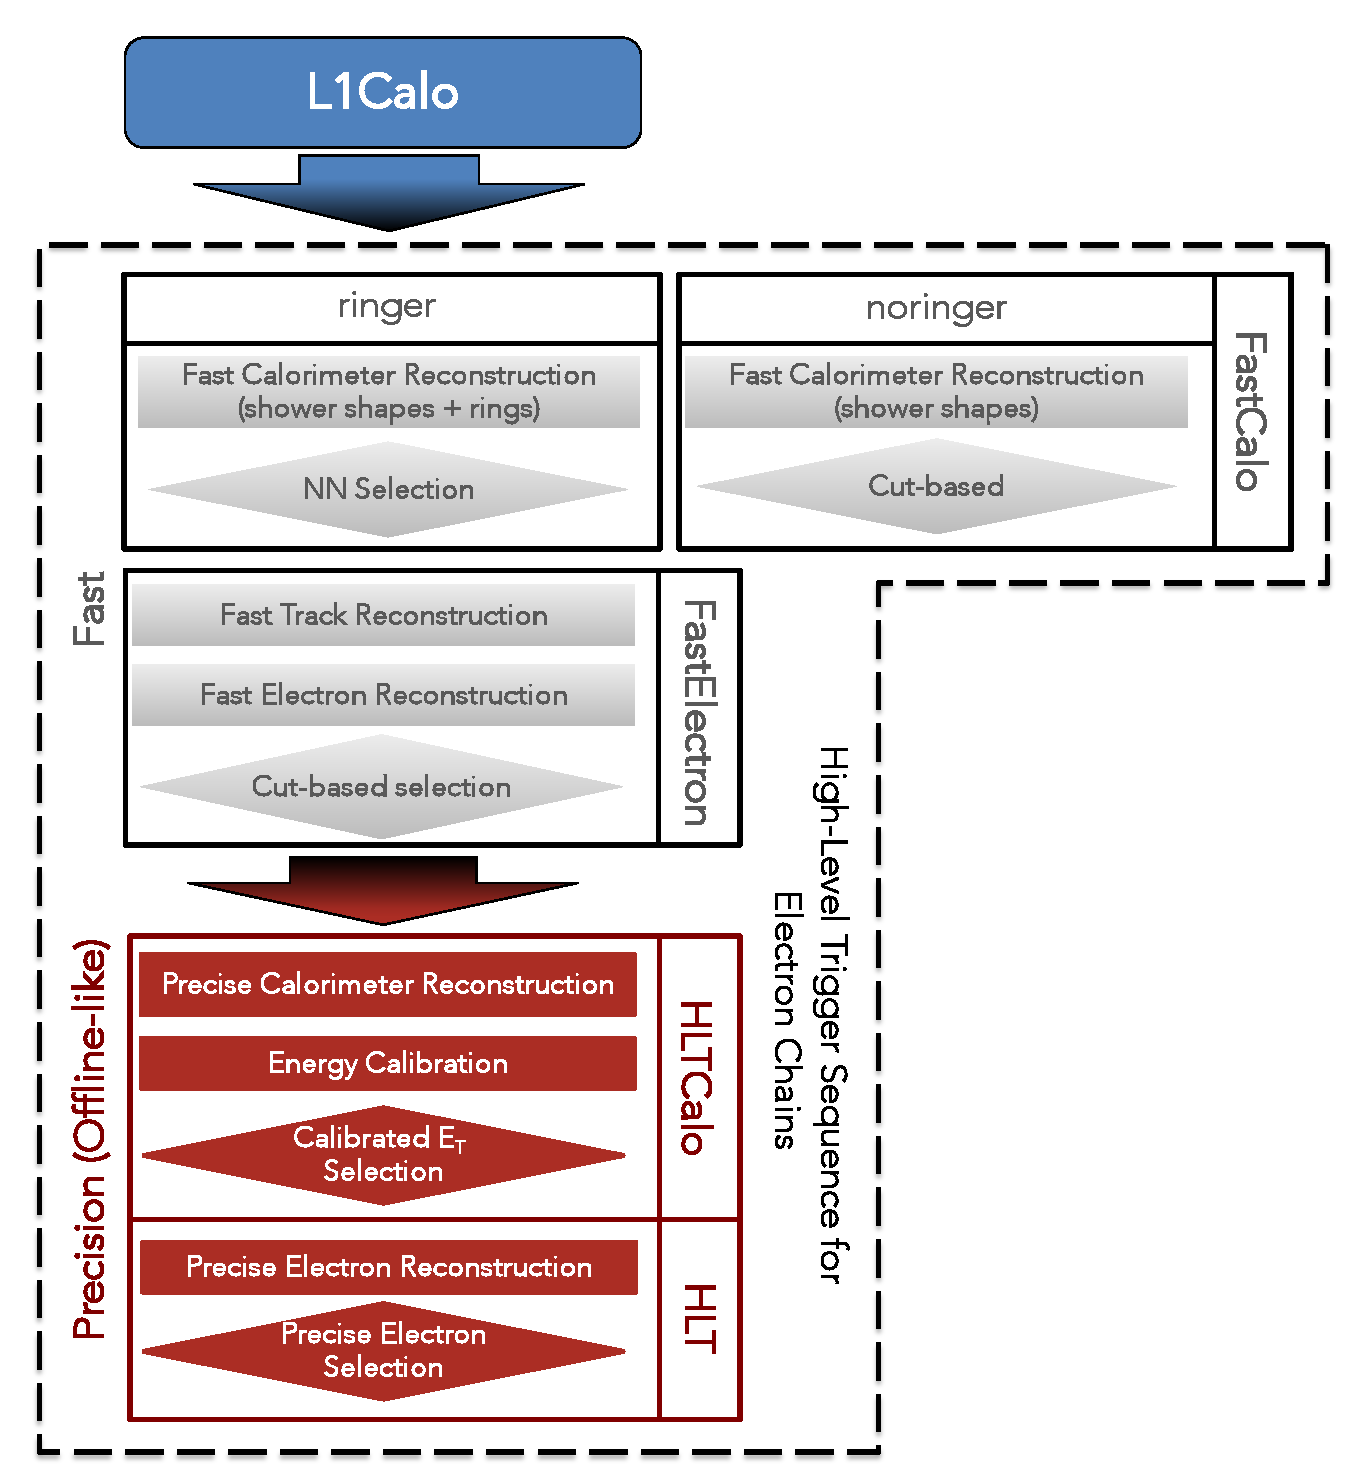
\includegraphics[width=0.7\textwidth]{sections/01_introduction/figures/ElectronChain_Run2_noringer_and_ringer.pdf}
  \caption{Chain of algorithms for electron triggers in the HLT. \DIFdelbeginFL \DIFdelFL{Difference }\DIFdelendFL \DIFaddbeginFL \DIFaddFL{Differences }\DIFaddendFL between \DIFaddbeginFL \DIFaddFL{the original }\DIFaddendFL baseline (no-ringer) and new (ringer) electron triggers lie \DIFdelbeginFL \DIFdelFL{on }\DIFdelendFL \DIFaddbeginFL \DIFaddFL{in }\DIFaddendFL the first step, \DIFdelbeginFL \DIFdelFL{the }\DIFdelendFL \DIFaddbeginFL \DIFaddFL{called }\DIFaddendFL FastCalo. \DIFdelbeginFL \DIFdelFL{Gray }\DIFdelendFL \DIFaddbeginFL \DIFaddFL{Grey }\DIFaddendFL blocks represent algorithms in the fast stage\DIFaddbeginFL \DIFaddFL{, }\DIFaddendFL and red blocks represent \DIFdelbeginFL \DIFdelFL{precision step }\DIFdelendFL \DIFaddbeginFL \DIFaddFL{precision-step }\DIFaddendFL algorithms.}
  \label{fig:electron_chain}
\end{figure}




This paper describes the performance improvements due to \DIFaddbegin \DIFadd{the }\DIFaddend introduction of the Neural-Ringer algorithm into the HLT fast \DIFdelbegin \DIFdel{calorimenter reconstruction step of the electron triggers, which }\DIFdelend \DIFaddbegin \DIFadd{calorimeter-reconstruction step for electron triggers. It }\DIFaddend became the baseline \DIFdelbegin \DIFdel{selection of }\DIFdelend \DIFaddbegin \DIFadd{algorithm for selecting }\DIFaddend events containing at least one isolated electron \DIFaddbegin \DIFadd{with transverse energy }\DIFaddend above 15\DIFaddbegin \DIFadd{~}\DIFaddend GeV in the 2017 \DIFdelbegin \DIFdel{proton-proton }\DIFdelend \DIFaddbegin \DIFadd{proton--proton }\DIFaddend collision ATLAS data-taking \DIFdelbegin \DIFdel{. The }\DIFdelend \DIFaddbegin \DIFadd{at $\sqs = 13$~TeV in LHC }\RunTwo\DIFadd{. }\DIFaddend Full details of its \DIFdelbegin \DIFdel{identification procedure are in Section~\ref{sec:neuralringer}}\DIFdelend \DIFaddbegin \DIFadd{electron identification procedure}\DIFaddend , including the training and tuning strategies\DIFdelbegin \DIFdel{. The online }\DIFdelend \DIFaddbegin \DIFadd{, are given in Section~\ref{sec:neuralringer}. Online }\DIFaddend performance results from the \rnn and \DIFdelbegin \DIFdel{the }\DIFdelend cut-based strategies are presented in Section~\ref{sec:operation}. \DIFdelbegin \DIFdel{A comparison of the }\DIFdelend \DIFaddbegin \DIFadd{The }\DIFaddend \rnn \DIFdelbegin \DIFdel{with the }\DIFdelend \DIFaddbegin \DIFadd{and }\DIFaddend cut-based \DIFdelbegin \DIFdel{triggers }\DIFdelend \DIFaddbegin \DIFadd{electron triggers are compared from an offline perspective }\DIFaddend using statistical methods \DIFdelbegin \DIFdel{through the offline perspective is performed }\DIFdelend in Section~\ref{sec:off_ana}. Finally, the conclusions and prospects 
are \DIFdelbegin \DIFdel{derived }\DIFdelend \DIFaddbegin \DIFadd{presented }\DIFaddend in Section~\ref{sec:conclusion}.
 \newpage  % ok
 \newpage \section{The \rnn{} \DIFdelbegin \DIFdel{Algorithm}\DIFdelend \DIFaddbegin \DIFadd{algorithm}\DIFaddend }%
\label{sec:neuralringer}


Instead of using electron \DIFdelbegin \DIFdel{shower shapes }\DIFdelend \DIFaddbegin \DIFadd{shower-shape }\DIFaddend variables~\cite{TRIG-2018-05} to discriminate \DIFdelbegin \DIFdel{electrons from }\DIFdelend \DIFaddbegin \DIFadd{between electrons and }\DIFaddend background, the Neural-Ringer algorithm \DIFdelbegin \DIFdel{adapt another shower representation made of transverse energy rings built from the sum of calorimeter cells }\DIFdelend \DIFaddbegin \DIFadd{adopts a shower representation consisting of rings of transverse energy, built from sums of calorimeter-cell energies, }\DIFaddend around each candidate provided as \DIFaddbegin \DIFadd{an }\DIFaddend RoI by the L1 trigger. The distribution of those energy sums is used by \DIFdelbegin \DIFdel{an }\DIFdelend \DIFaddbegin \DIFadd{a }\DIFaddend set of neural networks to \DIFdelbegin \DIFdel{classify }\DIFdelend \DIFaddbegin \DIFadd{distinguish }\DIFaddend electrons from background. This section \DIFdelbegin \DIFdel{is dedicated to }\DIFdelend \DIFaddbegin \DIFadd{describes }\DIFaddend the Neural-Ringer algorithm.

\subsection{The ATLAS \DIFdelbegin \DIFdel{Calorimeter}\DIFdelend \DIFaddbegin \DIFadd{calorimeters}\DIFaddend }

The ATLAS \DIFdelbegin \DIFdel{uses a right-handed coordinate system with its origin at the nominal interaction point (IP) in the centre of the detector and the z-axis along the beam-pipe. The x-axis points from the IP to the centre of the LHC ring, and the y-axis points upward. Cylindrical coordinates (r, $\phi$) are used in the transverse plane, \phi being the azimuthal angle around the beam-pipe. The pseudorapidity is defined in terms of the polar angle $\theta$ as \eta = -$\ln{tan(\theta/2)}$. The angular distance $\Delta R$ is defined as $\Delta R = \sqrt{(\Delta\eta)^{2} + (\Delta\phi)^{2}}$ . Transverse momenta and energies are defined as $pT = p\sin\theta$ and $E_{T}$ = $E\sin\theta$, respectively.
}%DIFDELCMD < 

%DIFDELCMD < %%%
\DIFdel{The ATLAS }\DIFdelend calorimeters comprise rectangular cells in the
\etaphi plane\DIFaddbegin \footnote{\DIFadd{ATLAS uses a right-handed coordinate system with its origin at the nominal interaction point (IP) in the centre of the detector and the $z$-axis along the beam-pipe. The $x$-axis points from the IP to the centre of the LHC ring, and the $y$-axis points upward. Cylindrical coordinates ($r$, $\phi$) are used in the transverse plane, \phi being the azimuthal angle around the beam-pipe. The pseudorapidity is defined in terms of the polar angle $\theta$ as $\eta = -\ln{\tan(\theta/2)}$. The angular distance $\Delta R$ is defined as $\Delta R = \sqrt{(\Delta\eta)^{2} + (\Delta\phi)^{2}}$ . Transverse momenta and energies are defined as $\pT = p\sin\theta$ and $\ET = E\sin\theta$, respectively.}} \DIFaddend for different layers in depth, except for the forward calorimeters. The calorimeter system covers the pseudorapidity range \(|\eta| < 4.9\)~\cite{PERF-2007-01}. Within the region $|\eta|< 3.2$, \DIFdelbegin \DIFdel{an electromagnetic calorimetry (ECAL) }\DIFdelend \DIFaddbegin \DIFadd{electromagnetic calorimetry }\DIFaddend is provided by \DIFdelbegin \DIFdel{the }\DIFdelend \DIFaddbegin \DIFadd{a }\DIFaddend high-granularity lead/\DIFdelbegin \DIFdel{Liquid-Argon }\DIFdelend \DIFaddbegin \DIFadd{liquid-argon }\DIFaddend (LAr) \DIFdelbegin \DIFdel{calorimeters constituted }\DIFdelend \DIFaddbegin \DIFadd{calorimeter (ECal) composed }\DIFaddend of barrel (EMB1,2,3) \DIFdelbegin \DIFdel{and end-cap }\DIFdelend \DIFaddbegin \DIFadd{sections covering $|\eta|<1.475$ and endcap }\DIFaddend (EMEC1,2,3) \DIFaddbegin \DIFadd{sections covering $1.375<|\eta|<3.2$}\DIFaddend , with an additional thin LAr presampler (\ps) covering the barrel (PreSamplerB) and \DIFdelbegin \DIFdel{end-cap }\DIFdelend \DIFaddbegin \DIFadd{endcap }\DIFaddend (PreSamplerE) \DIFdelbegin \DIFdel{, in order }\DIFdelend \DIFaddbegin \DIFadd{regions }\DIFaddend to correct for energy losses in \DIFdelbegin \DIFdel{material upstream of the calorimeters}\DIFdelend \DIFaddbegin \DIFadd{upstream material}\DIFaddend ~\cite{LARG-2009-01,larg_tdr}. \DIFdelbegin \DIFdel{The Hadronic calorimetry (HCAL) }\DIFdelend \DIFaddbegin \DIFadd{Hadronic calorimetry within $|\eta|< 3.2$ }\DIFaddend is provided by \DIFdelbegin \DIFdel{the }\DIFdelend \DIFaddbegin \DIFadd{a }\DIFaddend steel/\DIFdelbegin \DIFdel{scintillating-tile }\DIFdelend \DIFaddbegin \DIFadd{scintillator-tile }\DIFaddend calorimeter (\tilecal)~\cite{TCAL-2017-01,tile_tdr} \DIFdelbegin \DIFdel{, constituted }\DIFdelend \DIFaddbegin \DIFadd{composed }\DIFaddend of three barrel \DIFdelbegin \DIFdel{structures }\DIFdelend \DIFaddbegin \DIFadd{sections }\DIFaddend (TileBar0,\DIFdelbegin \DIFdel{TileBar1 and TileBar2) within $|\eta| < 1.0$}\DIFdelend \DIFaddbegin \DIFadd{1}\DIFaddend ,\DIFaddbegin \DIFadd{2) covering $|\eta| < 1.0$ and }\DIFaddend three extended barrel \DIFdelbegin \DIFdel{structures }\DIFdelend \DIFaddbegin \DIFadd{sections }\DIFaddend (TileExt1,2,3) covering \DIFdelbegin \DIFdel{the region of }\DIFdelend $0.8<|\eta|< 1.7$\DIFaddbegin \DIFadd{, }\DIFaddend and two copper/LAr hadronic endcap calorimeters (HEC)~\cite{cal_tdr} \DIFdelbegin \DIFdel{within $1.5<|\eta|< 3.2$ divided in }\DIFdelend \DIFaddbegin \DIFadd{divided into }\DIFaddend four modules (HEC0,1,2,3) \DIFaddbegin \DIFadd{covering $1.5<|\eta|< 3.2$}\DIFaddend . Transition regions between calorimeters are used \DIFdelbegin \DIFdel{to locate }\DIFdelend \DIFaddbegin \DIFadd{as locations for }\DIFaddend detector services and induce \DIFdelbegin \DIFdel{a sharing of showers between calorimetersthat }\DIFdelend \DIFaddbegin \DIFadd{shower-sharing between calorimeters, which }\DIFaddend degrades energy measurements in those regions. Here, the \DIFdelbegin \DIFdel{transition from the barrel to the endcap }\DIFdelend \DIFaddbegin \DIFadd{barrel-to-endcap transition }\DIFaddend is complemented by the intermediate tile calorimeter (ITC)\DIFdelbegin \DIFdel{composed by }\DIFdelend \DIFaddbegin \DIFadd{, which is composed of }\DIFaddend two modules (TileGap1,2,3) that are \DIFdelbegin \DIFdel{both attached on the face of the external barrel }\DIFdelend \DIFaddbegin \DIFadd{attached to the external faces of the barrel and are used }\DIFaddend to estimate signal losses~\cite{cal_tdr}. The \DIFdelbegin \DIFdel{solid angle }\DIFdelend \DIFaddbegin \DIFadd{solid-angle }\DIFaddend coverage is completed with forward
copper/LAr and tungsten/LAr calorimeter (FCal) modules \DIFdelbegin \DIFdel{optimised }\DIFdelend \DIFaddbegin \DIFadd{optimized }\DIFaddend for electromagnetic (EM) and hadronic (HAD) measurements, respectively. The \DIFdelbegin \DIFdel{specified calorimeters
provide }\DIFdelend \DIFaddbegin \DIFadd{calorimeter system
provides }\DIFaddend full azimuthal ($\phi$) coverage with a total of about 190\DIFdelbegin \DIFdel{,}\DIFdelend \DIFaddbegin \DIFadd{\,}\DIFaddend 000 readout cells. 



The electromagnetic and hadronic calorimeters are segmented~\cite{PERF-2007-01} \DIFdelbegin \footnote{\DIFdel{The two
central layers in HCAL end-cap are summed to result in a single measurement.}} %DIFAUXCMD
\addtocounter{footnote}{-1}%DIFAUXCMD
\DIFdelend longitudinally (i.e.\DIFaddbegin \DIFadd{\ }\DIFaddend in depth) into three\DIFdelbegin \DIFdel{sampling layers }\DIFdelend \DIFaddbegin \footnote{\DIFadd{The two central layers of each hadronic endcap calorimeter are summed to provide a single measurement.}} \DIFadd{sampling layers, }\DIFaddend where each layer has its own lateral ($\eta\times\phi$) granularity. \DIFdelbegin \DIFdel{Besides granularity, the amount of detector }\DIFdelend \DIFaddbegin \DIFadd{The amount of }\DIFaddend material in front of \DIFdelbegin \DIFdel{the detector in }\DIFdelend each sampling layer \DIFdelbegin \DIFdel{also }\DIFdelend varies with \abseta, leading to variations in the expected lateral and longitudinal \DIFdelbegin \DIFdel{profiles. Additionally, the expected profile is also dependent }\DIFdelend \DIFaddbegin \DIFadd{shower profiles. The expected profiles also depend }\DIFaddend on the physics object\DIFaddbegin \DIFadd{'s }\DIFaddend total energy. In the EM calorimeter, most of the EM shower energy is collected in the second layer (EM2), while the third layer (EM3) provides measurements of energy deposited \DIFdelbegin \DIFdel{in }\DIFdelend \DIFaddbegin \DIFadd{by }\DIFaddend the shower tails. \DIFdelbegin \DIFdel{Although, it is important to mention }\DIFdelend \DIFaddbegin \DIFadd{However, it should be noted }\DIFaddend that the first EM layer (EM1) plays an important role in \DIFdelbegin \DIFdel{the discrimination of electrons against }\DIFdelend \DIFaddbegin \DIFadd{discriminating between electrons and }\DIFaddend $\pi^0$ \DIFaddbegin \DIFadd{mesons}\DIFaddend . The hadronic calorimeters, which surround the EM detectors, provide additional \DIFaddbegin \DIFadd{electron }\DIFaddend discrimination power through \DIFdelbegin \DIFdel{further }\DIFdelend energy measurements of possible EM shower tails, as well as rejection of events with activity of hadronic origin \DIFdelbegin \DIFdel{with }\DIFdelend \DIFaddbegin \DIFadd{via the }\DIFaddend three sampling layers (HAD1,2,3). 


\subsection{Building the \DIFdelbegin \DIFdel{Rings}\DIFdelend \DIFaddbegin \DIFadd{rings}\DIFaddend }\label{ssec:rnn_for_online_and_eletrons}


\DIFdelbegin \DIFdel{The }\DIFdelend \DIFaddbegin \DIFadd{Since the }\DIFaddend Neural-Ringer algorithm was \DIFdelbegin \DIFdel{considered }\DIFdelend \DIFaddbegin \DIFadd{designed }\DIFaddend to operate online \DIFdelbegin \DIFdel{at }\DIFdelend \DIFaddbegin \DIFadd{in software at the }\DIFaddend \fastcalo{} stage\DIFdelbegin \DIFdel{in software}\DIFdelend , approximations were made. Specifically, \DIFdelbegin \DIFdel{the }\DIFdelend rectangular rings are constructed to match the grid layout of the calorimeter cells\DIFaddbegin \DIFadd{, }\DIFaddend and the ring coverage is bounded by the RoI\DIFaddbegin \DIFadd{'s }\DIFaddend area. In addition, granularity changes \DIFdelbegin \DIFdel{from the cell sizes from }\DIFdelend \DIFaddbegin \DIFadd{due to different cell sizes in }\DIFaddend different regions of the detector are neglected in order to employ a grid-like algorithm. \DIFdelbegin \DIFdel{Here, }\DIFdelend \DIFaddbegin \DIFadd{When }\DIFaddend considering only the EM1 layer, the $\eta$\DIFdelbegin \DIFdel{granularity }\DIFdelend \DIFaddbegin \DIFadd{-granularity }\DIFaddend used by the algorithm is 0.003 for the entire \DIFdelbegin \DIFdel{eta }\DIFdelend \DIFaddbegin \DIFadd{$\eta$ }\DIFaddend range defined ($|\eta|<2.5$)\DIFdelbegin \DIFdel{. However, the detector construction at this layer cover the region of }\DIFdelend \DIFaddbegin \DIFadd{, although this layer actually covers the region }\DIFaddend $0<|\eta|<2.37$ and has \DIFdelbegin \DIFdel{different granularities in }\DIFdelend \DIFaddbegin \DIFadd{three different }\DIFaddend $\eta$\DIFdelbegin \DIFdel{: starts with }\DIFdelend \DIFaddbegin \DIFadd{-granularities: }\DIFaddend 0.003 \DIFdelbegin \DIFdel{at }\DIFdelend \DIFaddbegin \DIFadd{for }\DIFaddend $0<|\eta|<1.81$\DIFdelbegin \DIFdel{; }\DIFdelend \DIFaddbegin \DIFadd{, }\DIFaddend 0.004 \DIFdelbegin \DIFdel{at }\DIFdelend \DIFaddbegin \DIFadd{for }\DIFaddend $1.81<|\eta|<2.01$ and 0.006 at $2.01<|\eta|<2.37$.


\DIFdelbegin \DIFdel{Here, the algorithm}\DIFdelend \DIFaddbegin \DIFadd{The algorithm's }\DIFaddend RoI covers a \DIFdelbegin \DIFdel{region of the calorimeter, centered in the L1 provided RoI, of
}\DIFdelend \DIFaddbegin \DIFadd{calorimeter region of }\DIFaddend $0.4\times0.4$ in the $\eta\times\phi$ plane\DIFaddbegin \DIFadd{, centred on the L1-provided RoI}\DIFaddend . 
The algorithm starts \DIFdelbegin \DIFdel{on }\DIFdelend \DIFaddbegin \DIFadd{at }\DIFaddend the second EM sampling layer (EM2), where \DIFdelbegin \DIFdel{position given in }\DIFdelend \DIFaddbegin \DIFadd{the }\DIFaddend $\eta\times\phi$ \DIFdelbegin \DIFdel{plane }\DIFdelend \DIFaddbegin \DIFadd{position }\DIFaddend of the cell with \DIFdelbegin \DIFdel{highest $E_T$ on the algorithm}\DIFdelend \DIFaddbegin \DIFadd{the highest }\ET \DIFadd{in the algorithm's }\DIFaddend RoI is taken as the \DIFdelbegin \DIFdel{center }\DIFdelend \DIFaddbegin \DIFadd{centre }\DIFaddend of the cascade interaction in the calorimeter. The initial \DIFdelbegin \DIFdel{seed cell }\DIFdelend \DIFaddbegin \DIFadd{seed-cell }\DIFaddend position is propagated to other calorimeter layers in order to define the axis of the rings in \DIFdelbegin \DIFdel{that layer}\DIFdelend \DIFaddbegin \DIFadd{those layers}\DIFaddend . Then, for each layer, the algorithm refines the seed position \DIFdelbegin \DIFdel{searching for }\DIFdelend \DIFaddbegin \DIFadd{by searching for the }\DIFaddend most energetic cell inside \DIFdelbegin \DIFdel{of the }\DIFdelend \DIFaddbegin \DIFadd{a reconstruction }\DIFaddend window centred on the EM2 initial seed\DIFaddbegin \DIFadd{, }\DIFaddend and the energy deposition of an incoming particle is extracted by building concentric rings of cells, \DIFdelbegin \DIFdel{or simply ``rings''}\DIFdelend \DIFaddbegin \DIFadd{simply referred to as }\enquote{rings}\DIFaddend . 

\begin{figure}[h!t]
	\centering
	\begin{center}
		\begin{subfigure}[c]{.95\textwidth}
			\centering
			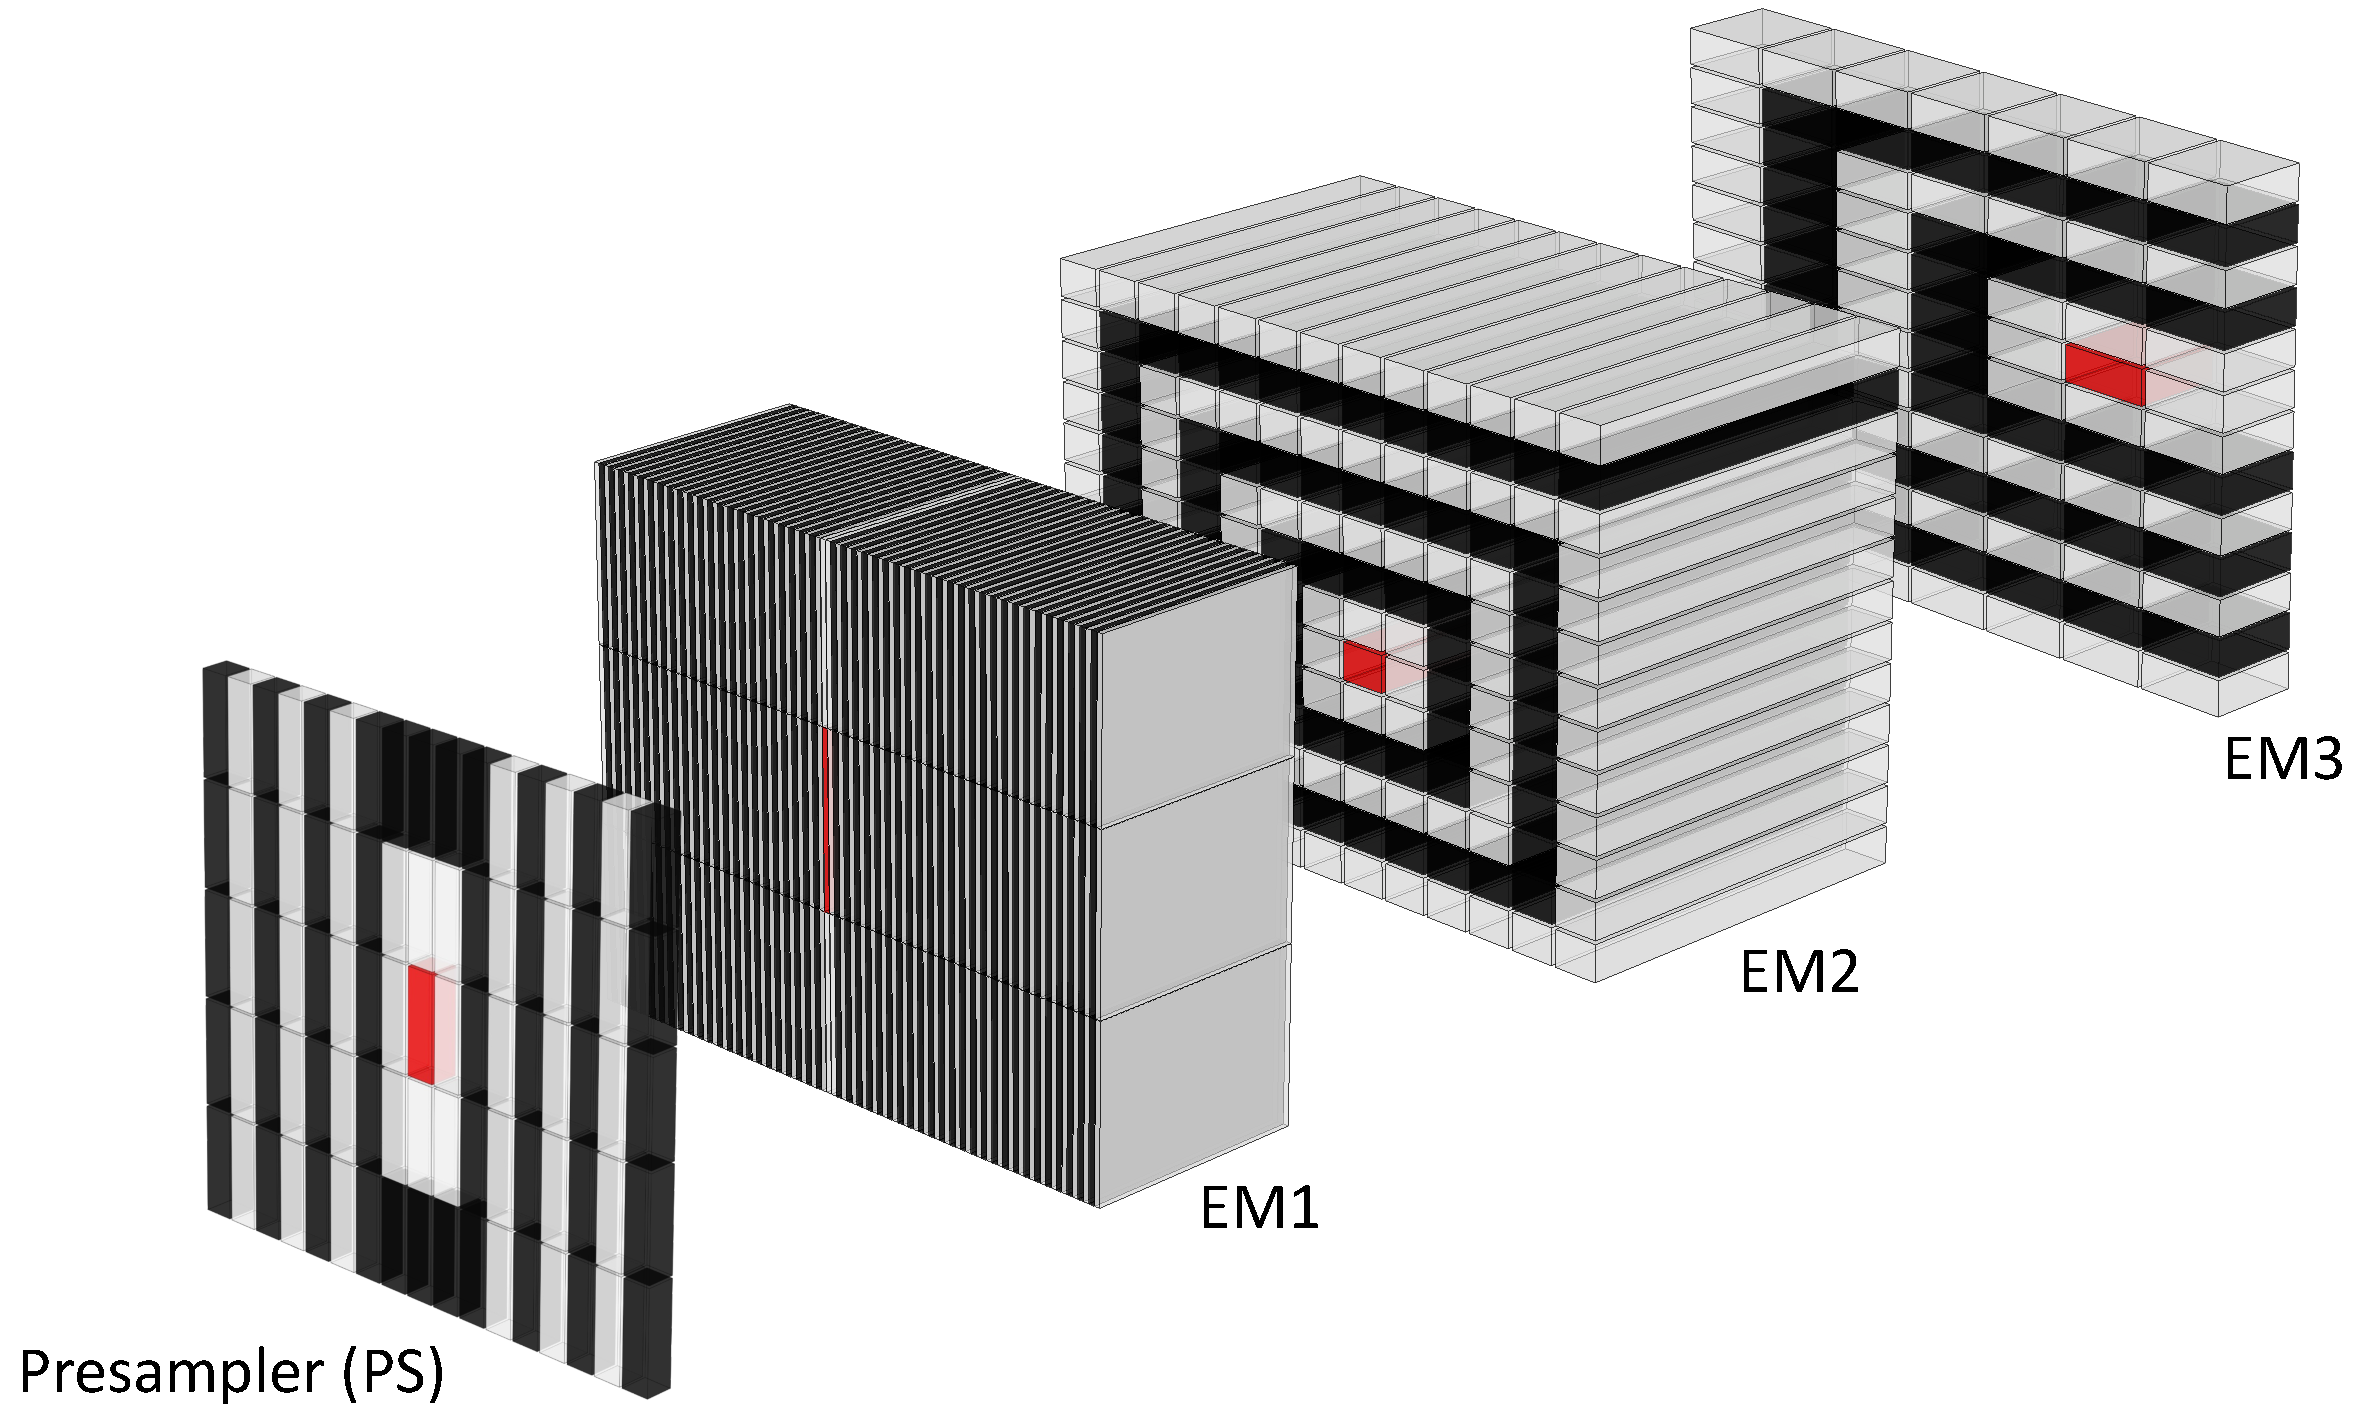
\includegraphics[width=\textwidth]{sections/02_ringer/figures/ATLAS_EM_Layers_v5.pdf}
			\caption{\DIFdelbeginFL \DIFdelFL{Eletromagnetic }\DIFdelendFL \DIFaddbeginFL \DIFaddFL{Electromagnetic }\DIFaddendFL calorimeter cells within the ringer reconstruction window.}
		\end{subfigure} \\
		\begin{subfigure}[c]{.95\textwidth}
			\centering
			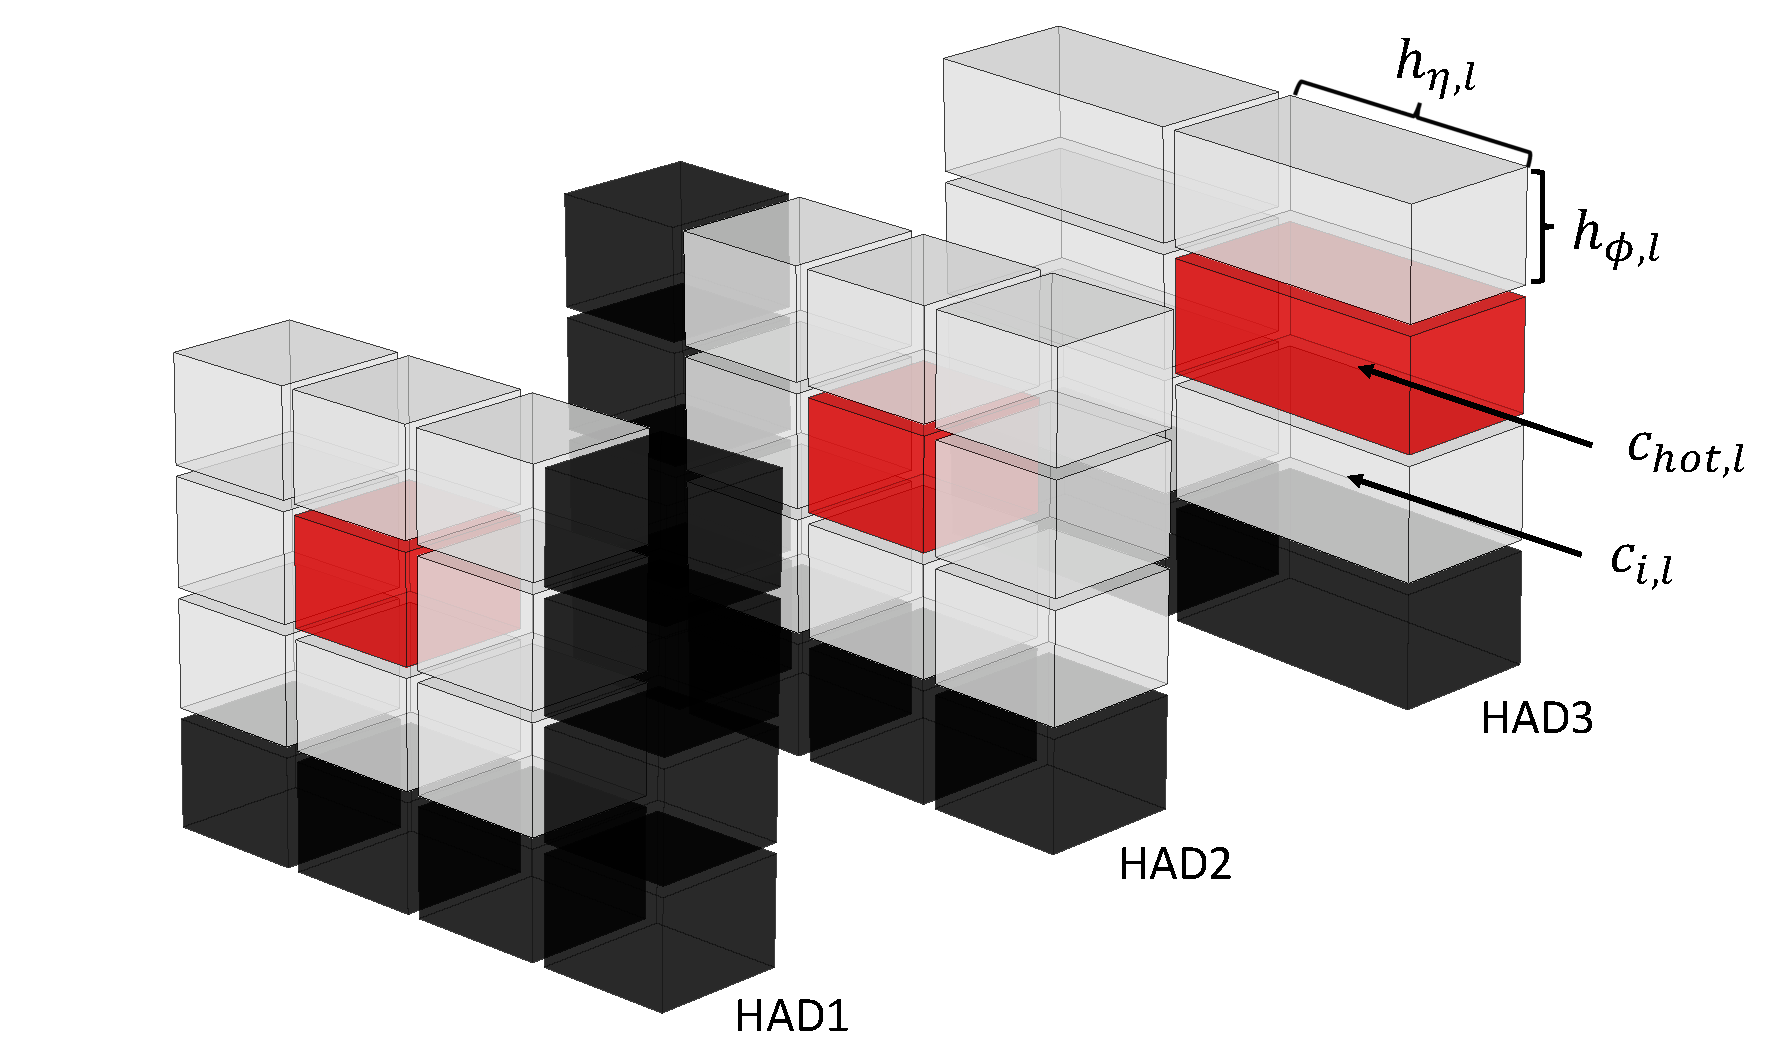
\includegraphics[width=\textwidth]{sections/02_ringer/figures/ATLAS_HAD_Layers_v5.pdf}
			\caption{Hadronic calorimeter cells within the ringer reconstruction window.}
		\end{subfigure}
	\end{center}
	\caption{\label{fig:calo_rings}
		Sketch \DIFdelbeginFL \DIFdelFL{to illustrate }\DIFdelendFL \DIFaddbeginFL \DIFaddFL{illustrating }\DIFaddendFL the ring-shaped energy description.
		The most energetic cell is in red, while the consecutive neighbouring rings are represented by alternating \DIFdelbeginFL \DIFdelFL{gray }\DIFdelendFL \DIFaddbeginFL \DIFaddFL{grey }\DIFaddendFL and black cells.
	}
\end{figure}

The refined seed (\DIFdelbegin \DIFdel{$c_{hot,l}$}\DIFdelend \DIFaddbegin \DIFadd{$c_{\text{hot},l}$}\DIFaddend ) is used as \DIFaddbegin \DIFadd{the }\DIFaddend starting point to build the rings. A ring $R_{n,l}$ contains all $C_{n,l}$ cells in calorimeter layer $l$ which are $n$ cells \DIFaddbegin \DIFadd{away }\DIFaddend from the refined seed (\DIFdelbegin \DIFdel{See }\DIFdelend \DIFaddbegin \DIFadd{see }\DIFaddend \figurename~\ref{fig:calo_rings} for an illustration of the parameters). Formally,


\DIFdelbegin \begin{displaymath}
%DIF < \label{eq:ring_idx}
\DIFdel{R_{n,l} = \left\{c_{n,l} \mid n = \left\lfloor \max{\left( 
\frac{| \eta_{i,l} - \eta_{hot,l} |}{h_{\eta,l}}, 
\frac{| \phi_{i,l} - \phi_{hot,l} |}{h_{\phi,l}} 
\right)} \right\rceil, 
\forall c_{i,l} \in
\Theta_{RoI,l}
\right\},
}\end{displaymath}%DIFAUXCMD
\DIFdelend \DIFaddbegin \begin{equation*}
%DIF > \label{eq:ring_idx}
\DIFadd{R_{n,l} = \left\{c_{n,l} \mid n = \left\lfloor \max{\left( 
\frac{| \eta_{i,l} - \eta_{\text{hot},l} |}{h_{\eta,l}}, 
\frac{| \phi_{i,l} - \phi_{\text{hot},l} |}{h_{\phi,l}} 
\right)} \right\rceil, 
\forall c_{i,l} \in
\Theta_{\text{RoI},l}
\right\},
}\end{equation*}\DIFaddend 



\noindent where (\DIFdelbegin \DIFdel{analogous to }\DIFdelend \DIFaddbegin \DIFadd{and analogously for }\DIFaddend $\phi$ when \DIFdelbegin \DIFdel{suitable) : }\DIFdelend \DIFaddbegin \DIFadd{appropriate) }\DIFaddend $\eta_{i,l}$
and \DIFdelbegin \DIFdel{$\eta_{hot,l}$ }\DIFdelend \DIFaddbegin \DIFadd{$\eta_{\text{hot},l}$ }\DIFaddend are respectively the $c_{i,l}$ and \DIFdelbegin \DIFdel{$c_{hot,l}$
cellsposition }\DIFdelend \DIFaddbegin \DIFadd{$c_{\text{hot},l}$
cells' positions }\DIFaddend in $\eta$;$h_{\eta,l}$ is the \DIFdelbegin \DIFdel{$l^{th}$ layer}\DIFdelend \DIFaddbegin \DIFadd{$l^{\text{th}}$ layer's }\DIFaddend cell size in $\eta$; \DIFdelbegin \DIFdel{$\Theta_{RoI,l}$ }\DIFdelend \DIFaddbegin \DIFadd{$\Theta_{\text{RoI},l}$ }\DIFaddend is the set of cells
in the \DIFdelbegin \DIFdel{$l^{th}$ }\DIFdelend \DIFaddbegin \DIFadd{$l^{\text{th}}$ }\DIFaddend layer which are within the Ringer RoI\DIFaddbegin \DIFadd{; }\DIFaddend and $\lfloor \cdot \rceil$ is the \textit{round} function.
\tablename~\ref{tab:ring_alg_parameters} shows the number of rings computed at each layer and the respective granularity.


\begin{table}[ht!]
\centering
\caption{Nomenclature defining the \rnn{} algorithm layers and sections, as well as the respective parameters employed and \DIFaddbeginFL \DIFaddFL{the }\DIFaddendFL calorimeter sampling layers from which the cells are extracted. The \rnn{} algorithm parameters were dependent on the ringer layer $l$ \DIFdelbeginFL \DIFdelFL{and }\DIFdelendFL \DIFaddbeginFL \DIFaddFL{but }\DIFaddendFL independent \DIFdelbeginFL \DIFdelFL{on }\DIFdelendFL \DIFaddbeginFL \DIFaddFL{of }\DIFaddendFL \eta{} and \et{} during \DIFdelbeginFL \DIFdelFL{Run~2. }\DIFdelendFL \DIFaddbeginFL \DIFaddFL{LHC }\RunTwo\DIFaddFL{. }\DIFaddendFL The parameters are the ring size in \eta{} ($h_{\eta,l}$), $\phi$ ($h_{\phi,l}$) and the number of rings to be computed in each layer (\DIFdelbeginFL \DIFdelFL{$\text{N}_l$}\DIFdelendFL \DIFaddbeginFL \DIFaddFL{$N_l$}\DIFaddendFL ).
}%
\label{tab:ring_alg_parameters}
\DIFdelbeginFL %DIFDELCMD < \resizebox{.8\textwidth}{!}{%
%DIFDELCMD < \begin{tabular}{lc|ccc|ccc}
%DIFDELCMD < \hline
%DIFDELCMD < \hline
%DIFDELCMD < \multicolumn{2}{c|}{Ringer} & \multicolumn{3}{c|}{Calorimeter Sampling} & 
%DIFDELCMD < \multicolumn{3}{c}{Parameters} \\
%DIFDELCMD < \hline
%DIFDELCMD < Section & Layer ($l$) & Barrel & \itc & End-cap & $h_{\etaa,l}$ & $h_{\phii,l}$ & $N_l$ \\
%DIFDELCMD < \hline
%DIFDELCMD < \hline
%DIFDELCMD < \multirow{4}*{EM} & \ps &  \presamplerb & & \presamplere & 0.025 & 0.1 & 8 \\
%DIFDELCMD < \cline{2-5}
%DIFDELCMD < & \emi & \emb{1} &  & \emec{1} & 0.003 & 0.1 & 64  \\
%DIFDELCMD < \cline{3-5}
%DIFDELCMD < & \emii & \emb{2} &  & \emec{2} & 0.025 & 0.025 & 8 \\
%DIFDELCMD < \cline{3-5}
%DIFDELCMD < & \emiii & \emb{3} &  & \emec{3} & 0.050 & 0.025 & 8 \\
%DIFDELCMD < \cline{1-5}
%DIFDELCMD < \multirow{6}*{HAD} & \multirow{2}*{\hadi} & \tilebar{0} &
%DIFDELCMD < \multirow{2}*{\tilegap{3}} & \multirow{2}*{\hec{0}} & \multirow{2}*{0.1} & \multirow{2}*{0.1} & \multirow{2}*{4} \\
%DIFDELCMD < &                     & \tileext{0} &                               &                           \\
%DIFDELCMD < \cline{3-5}
%DIFDELCMD < & \multirow{2}*{\hadii} & \tilebar{1} & \multirow{2}*{\tilegap{1}} & \hec{1}       & \multirow{2}*{0.1} & \multirow{2}*{0.1} & \multirow{2}*{4} \\
%DIFDELCMD < &                   & \tileext{1} &              & \hec{2}  \\
%DIFDELCMD < \cline{3-5}
%DIFDELCMD < & \multirow{2}*{\hadiii} & \tilebar{2} & \multirow{2}*{\tilegap{2}} & \multirow{2}*{\hec{3}} & \multirow{2}*{0.2} & \multirow{2}*{0.1} & \multirow{2}*{4} \\
%DIFDELCMD < &                     & \tileext{2} &                &             \\
%DIFDELCMD < \hline
%DIFDELCMD < \hline
%DIFDELCMD < \end{tabular}
%DIFDELCMD < }
%DIFDELCMD < %%%
\DIFdelendFL \DIFaddbeginFL \resizebox{.8\textwidth}{!}{%
\begin{tabular}{lc|ccc|ccc}
\hline
\hline
\multicolumn{2}{c|}{Ringer} & \multicolumn{3}{c|}{Calorimeter Sampling} & 
\multicolumn{3}{c}{Parameters} \\
\hline
Section & Layer ($l$) & Barrel & \itc & End-cap & $h_{\etaa,l}$ & $h_{\phii,l}$ & $N_l$ \\
\hline
\hline
\multirow{4}*{EM} & \ps &  \presamplerb & & \presamplere & ~0.025 & 0.1~~ & ~8 \\
\cline{2-5}
& \emi & \emb{1} &  & \emec{1} & ~0.003 & 0.1~~ & 64~  \\
\cline{3-5}
& \emii & \emb{2} &  & \emec{2} & ~0.025 & ~~0.025 & ~8 \\
\cline{3-5}
& \emiii & \emb{3} &  & \emec{3} & ~0.050 & ~~0.025 & ~8 \\
\cline{1-5}
\multirow{6}*{HAD} & \multirow{2}*{\hadi} & \tilebar{0} &
\multirow{2}*{\tilegap{3}} & \multirow{2}*{\hec{0}} & \multirow{2}*{0.1~~~} & \multirow{2}*{0.1~~} & \multirow{2}*{~4} \\
&                     & \tileext{0} &                               &                           \\
\cline{3-5}
& \multirow{2}*{\hadii} & \tilebar{1} & \multirow{2}*{\tilegap{1}} & \hec{1}       & \multirow{2}*{0.1~~~} & \multirow{2}*{0.1~~} & \multirow{2}*{~4} \\
&                   & \tileext{1} &              & \hec{2}  \\
\cline{3-5}
& \multirow{2}*{\hadiii} & \tilebar{2} & \multirow{2}*{\tilegap{2}} & \multirow{2}*{\hec{3}} & \multirow{2}*{0.2~~~} & \multirow{2}*{0.1~~} & \multirow{2}*{~4} \\
&                     & \tileext{2} &                &             \\
\hline
\hline
\end{tabular}
}
\DIFaddendFL \end{table}

The \DIFdelbegin \DIFdel{sum }\DIFdelend \DIFaddbegin \DIFadd{sums }\DIFaddend of the transverse energies of cells $c_{n,l}$ in the \DIFdelbegin \DIFdel{ring }\DIFdelend \DIFaddbegin \DIFadd{rings }\DIFaddend $R_{n,l}$ form a vector of discriminating quantities. They are ordered \DIFdelbegin \DIFdel{outwards and }\DIFdelend \DIFaddbegin \DIFadd{laterally outwards and longitudinally }\DIFaddend from the innermost \DIFaddbegin \DIFadd{to outermost }\DIFaddend layer of the calorimeter\DIFdelbegin \DIFdel{and provide }\DIFdelend \DIFaddbegin \DIFadd{, thus providing }\DIFaddend the ring-shaped information \DIFdelbegin \DIFdel{of }\DIFdelend \DIFaddbegin \DIFadd{about }\DIFaddend the RoI.




The \DIFdelbegin \DIFdel{ring building }\DIFdelend \DIFaddbegin \DIFadd{ring-building }\DIFaddend process results in \DIFaddbegin \DIFadd{a total of }\DIFaddend 100 rings \DIFdelbegin \DIFdel{in total }\DIFdelend across all calorimeter layers in each RoI. \DIFdelbegin \DIFdel{Thereby, a dimensionality reduction is provided }\DIFdelend \DIFaddbegin \DIFadd{Well-known features of EM shower physics allow a large reduction in dimensionality to be achieved }\DIFaddend by compacting the typical input space \DIFdelbegin \DIFdel{dimensionality }\DIFdelend of approximately 1000--1200 cells per ROI into \DIFdelbegin \DIFdel{the above-mentioned }\DIFdelend \DIFaddbegin \DIFadd{these }\DIFaddend 100 rings\DIFdelbegin \DIFdel{through the usage of EM shower physics knowledge}\DIFdelend : the rings can keep a complete description of the \DIFdelbegin \DIFdel{symmetric lateral and longitudinal }\DIFdelend \DIFaddbegin \DIFadd{longitudinal and symmetric lateral }\DIFaddend information. However, the algorithm only approximates this concept in order to meet the online operation requirements and avoid further manipulation of the \DIFdelbegin \DIFdel{instrumented }\DIFdelend \DIFaddbegin \DIFadd{instrumental }\DIFaddend information. 
Figure~\ref{fig:rings_profile} shows the ring-shaped mean profile differences between electrons and jet particles. 



\begin{figure}[!ht]
  \centering
  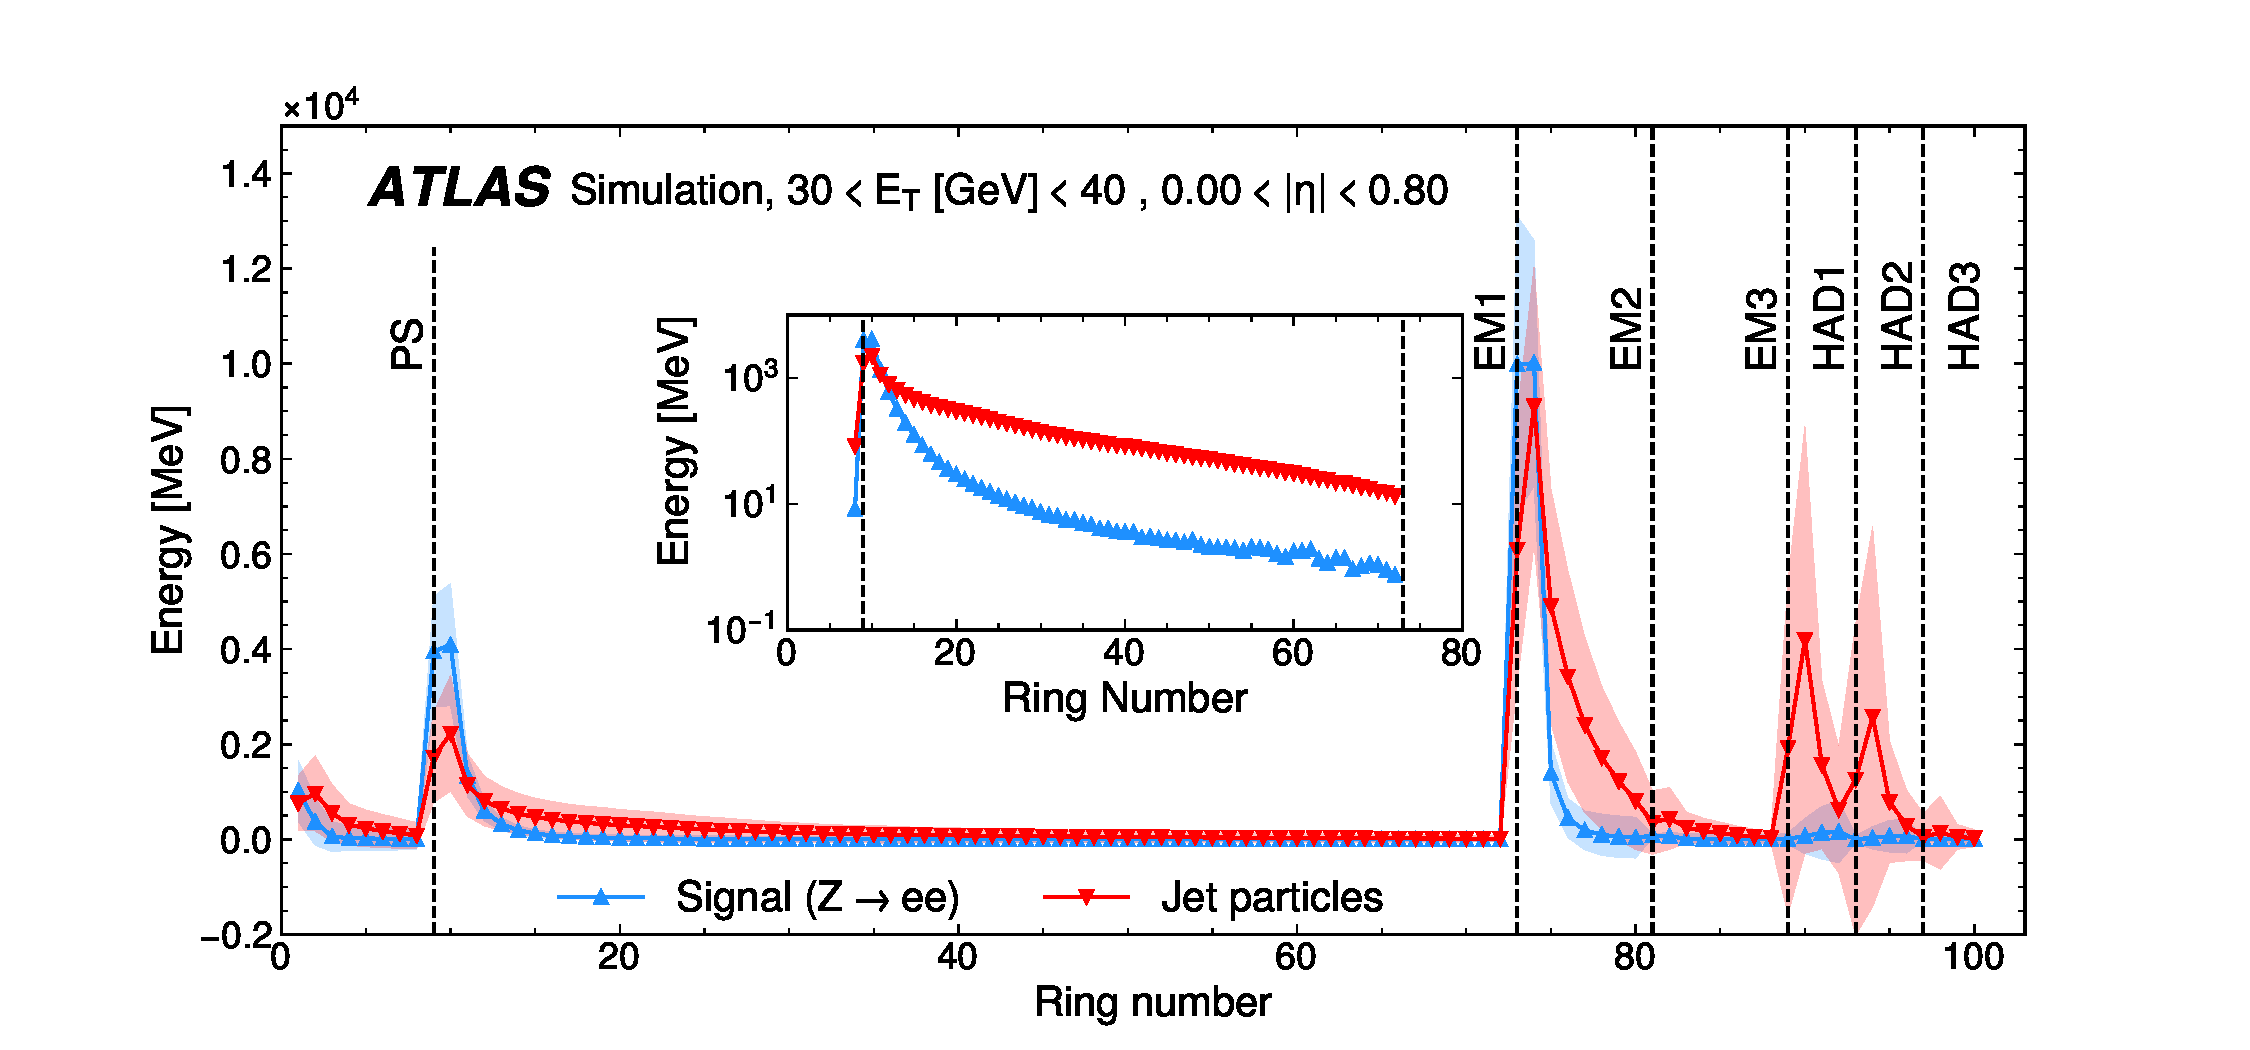
\includegraphics[width=0.9\textwidth]{sections/02_ringer/figures/ring_shape.pdf}
  \caption{Average ring profile from \DIFdelbeginFL \DIFdelFL{collision }\DIFdelendFL \DIFaddbeginFL \DIFaddFL{simulation }\DIFaddendFL data at \DIFdelbeginFL \DIFdelFL{$30 \leq E_T < 40$ }\DIFdelendFL \DIFaddbeginFL \DIFaddFL{$30 \leq \ET < 40$~}\DIFaddendFL GeV and $0.0 \leq \eta < 0.8$ for each layer of the calorimeter. The \DIFdelbeginFL \DIFdelFL{embedded }\DIFdelendFL profile \DIFaddbeginFL \DIFaddFL{in the inset }\DIFaddendFL shows the \DIFdelbeginFL \DIFdelFL{EM1 layer }\DIFdelendFL \DIFaddbeginFL \DIFaddFL{EM1-layer }\DIFaddendFL ring energies \DIFdelbeginFL \DIFdelFL{in }\DIFdelendFL \DIFaddbeginFL \DIFaddFL{on }\DIFaddendFL a logarithmic scale. Most \DIFdelbeginFL \DIFdelFL{part }\DIFdelendFL of the energy \DIFdelbeginFL \DIFdelFL{for }\DIFdelendFL \DIFaddbeginFL \DIFaddFL{of }\DIFaddendFL the electrons is absorbed by the \DIFdelbeginFL \DIFdelFL{eletromagnetic }\DIFdelendFL \DIFaddbeginFL \DIFaddFL{electromagnetic }\DIFaddendFL layers. For the jets, most of the energy is absorbed by the hadronic layers.}
  \label{fig:rings_profile}
\end{figure}

\subsubsection{Ring \DIFdelbegin \DIFdel{Sums }\DIFdelend \DIFaddbegin \DIFadd{sums }\DIFaddend as \DIFdelbegin \DIFdel{Discriminant Variables}\DIFdelend \DIFaddbegin \DIFadd{discriminating variables}\DIFaddend }

The current strategy concatenates all rings \DIFdelbegin \DIFdel{in }\DIFdelend \DIFaddbegin \DIFadd{into }\DIFaddend a single vector of 100
variables. \DIFdelbegin \DIFdel{An absolute normalization using }\DIFdelend \DIFaddbegin \DIFadd{The variables are normalized to the absolute value of }\DIFaddend the total RoI energy\DIFdelbegin \DIFdel{is applied to normalize the variables. 
This procedure was initially proposed and examined by~\mbox{%DIFAUXCMD
\cite{1995_seixas_ringer}}\hskip0pt%DIFAUXCMD
, as a way of preserving the shower energy profile in fractions of the total energy.The absolute value is used to avoid reflecting the values along the axis due to negative noise accumulation, a behavior which would impact the physics
representation of the normalized values and require a more complex decision
boundary}\DIFdelend \DIFaddbegin \DIFadd{, as shown in Eq.~(\ref{eq:ring_norm})}\DIFaddend :

\begin{equation}
  r^\prime_{k} = \frac{r_{k}}{| \sum\limits_{i=1}^{100} r_i
  |}, \;\;\;
    \forall \; k\in\{1,\dots,100\}\DIFdelbegin \DIFdel{.
}\DIFdelend \DIFaddbegin \DIFadd{,
}\DIFaddend \label{eq:ring_norm}
\end{equation}

\DIFdelbegin \DIFdel{Where }\DIFdelend \DIFaddbegin \DIFadd{where }\DIFaddend $r_k$ or $r_i$ is the sum of transverse energy of the cells in the ring with index $k$ or $i$\DIFaddbegin \DIFadd{, }\DIFaddend and $r^\prime_{k}$ is the normalized ring value with index $k$.
\DIFdelbegin \DIFdel{It is specially valuable for its simplicityas it uses of a non parametric }\DIFdelend \DIFaddbegin \DIFadd{The absolute value is used because of negative noise accumulation from some cells within the reconstruction window that were not excited by the particle shower.  This procedure was initially proposed and examined in Ref.~\mbox{%DIFAUXCMD
\cite{1995_seixas_ringer} }\hskip0pt%DIFAUXCMD
as a way of preserving the shower energy profile as fractions of the total energy. It is especially valuable because of its simplicity, since it uses a non-parametric }\DIFaddend approach, and for allowing easy interpretation of the shower profile.



\subsection{Motivation for \DIFaddbegin \DIFadd{using }\DIFaddend a \DIFdelbegin \DIFdel{Set }\DIFdelend \DIFaddbegin \DIFadd{set }\DIFaddend of \DIFdelbegin \DIFdel{Neural Networks}\DIFdelend \DIFaddbegin \DIFadd{neural networks}\DIFaddend }\label{ssec:nn_set}

The normalized concatenated ring vector \DIFdelbegin \DIFdel{feeds }\DIFdelend \DIFaddbegin \DIFadd{is fed into }\DIFaddend a set of \DIFdelbegin \DIFdel{Multi Layer Perceptrons (MLP). 
A single
model is drawn from the set for operation based on }\DIFdelend \DIFaddbegin \DIFadd{multi-layer perceptrons (MLPs). 
Each MLP corresponds to a model specifically trained for a particular region of }\eteta \DIFadd{space.
The model chosen for each shower's vector is }\DIFaddend the \DIFaddbegin \DIFadd{one trained for the }\DIFaddend nearest region \DIFdelbegin \DIFdel{on the }%DIFDELCMD < \eteta %%%
\DIFdel{spacefor which it was specific trained}\DIFdelend \DIFaddbegin \DIFadd{of phase space}\DIFaddend .

\DIFdelbegin \DIFdel{In regards to }\DIFdelend \DIFaddbegin \DIFadd{For }\DIFaddend calorimetry, the \DIFdelbegin \DIFdel{usage }\DIFdelend \DIFaddbegin \DIFadd{use }\DIFaddend of a set \DIFdelbegin \DIFdel{with specific modelsper phase space region allows to mitigate }\DIFdelend \DIFaddbegin \DIFadd{of models, each specific to a particular phase-space region, mitigates }\DIFaddend fluctuations in the \DIFdelbegin \DIFdel{variable }\DIFdelend \DIFaddbegin \DIFadd{variables' }\DIFaddend profiles
due to \DIFdelbegin \DIFdel{the detector responseand energy differences of the showers}\DIFdelend \DIFaddbegin \DIFadd{differences in shower energy and detector response}\DIFaddend .
A large contribution comes from \DIFdelbegin \DIFdel{granularity changes, which are discrete }\DIFdelend \DIFaddbegin \DIFadd{discrete detector-granularity changes }\DIFaddend in the phase space. Other important factors 
influencing such profiles are the
amount of the \DIFaddbegin \DIFadd{detector }\DIFaddend material as a function of \abseta{} and the \DIFdelbegin \DIFdel{dependency of underlying processes in the shower development with respect to the incoming
particle}\DIFdelend \DIFaddbegin \DIFadd{dependence of the
underlying shower-development processes on the incoming
particle's }\DIFaddend energy. Although \DIFdelbegin \DIFdel{these alterations }\DIFdelend \DIFaddbegin \DIFadd{the latter changes }\DIFaddend are mostly continuous, it is also
possible to approach the problem \DIFdelbegin \DIFdel{using }\DIFdelend \DIFaddbegin \DIFadd{via }\DIFaddend space discretization.

At the hardware resource level, splitting the training into multiple small models to accommodate \DIFdelbegin \DIFdel{inhomogeneity of the detector response }\DIFdelend \DIFaddbegin \DIFadd{detector response inhomogeneities }\DIFaddend speeds up the training cycle and allows \DIFdelbegin \DIFdel{to handle data }\DIFdelend \DIFaddbegin \DIFadd{data to be handled }\DIFaddend in memory, since only a small portion of the data is used to train \DIFdelbegin \DIFdel{that }\DIFdelend \DIFaddbegin \DIFadd{a }\DIFaddend specific model. Limiting the memory \DIFdelbegin \DIFdel{requirement }\DIFdelend \DIFaddbegin \DIFadd{required }\DIFaddend for tuning the models \DIFdelbegin \DIFdel{is particularly interesting }\DIFdelend \DIFaddbegin \DIFadd{was of particular interest }\DIFaddend in order to benefit from low-memory processing nodes, \DIFdelbegin \DIFdel{which were predominantly available in WLCG}\DIFdelend \DIFaddbegin \DIFadd{as these were the ones mostly available in the Worldwide LHC Computing Grid}\DIFaddend ~\cite{2015_lcg_tdr} during our \DIFdelbegin \DIFdel{developments}\DIFdelend \DIFaddbegin \DIFadd{development effort}\DIFaddend .\@ In addition, the decomposition of the problem can also lead to a reduction \DIFdelbegin \DIFdel{of the }\DIFdelend \DIFaddbegin \DIFadd{in }\DIFaddend training time~\cite{Polikar2006}, as observed heuristically
%\footnote{When using NVIDIA RTX 2080Ti in tensorflow 1.14 and a minibatch size of 1024, a MLP with single hidden layer, a substantial increase in the runtime (from 4 to 41 seconds per epoch) with respect to the set version was observed.} 
when comparing the tuning time of the set \DIFdelbegin \DIFdel{to a single model. 
Regarding the }\DIFdelend \DIFaddbegin \DIFadd{with that of a single overall model. 
With regard to }\DIFaddend operation, the proposed set only requires the choice of a
single model \DIFdelbegin \DIFdel{to operate instead of a more often committee machine approaches
that }\DIFdelend \DIFaddbegin \DIFadd{in order to operate, whereas the more common committee-machine approaches
}\DIFaddend require the computation of different models \DIFaddbegin \DIFadd{to run }\DIFaddend in parallel with a fusion
method~\cite{zhou_ensemble}.  Therefore, the chosen set configuration adds
minimal overhead in terms of trigger latency. Similarly, \DIFdelbegin \DIFdel{the }\DIFdelend \DIFaddbegin \DIFadd{our }\DIFaddend choice was to
\DIFdelbegin \DIFdel{operate with }\DIFdelend \DIFaddbegin \DIFadd{use }\DIFaddend low-complexity models, \DIFaddbegin \DIFadd{with }\DIFaddend a single hidden layer \DIFdelbegin \DIFdel{with }\DIFdelend \DIFaddbegin \DIFadd{and }\DIFaddend few neurons, to \DIFdelbegin \DIFdel{obtain a competitive method with respect to }\DIFdelend \DIFaddbegin \DIFadd{develop a method competitive with }\DIFaddend the cut-based approach \DIFdelbegin \DIFdel{, }\DIFdelend in terms of processing speed.



\subsection{Training and \DIFdelbegin \DIFdel{Decision Making }\DIFdelend \DIFaddbegin \DIFadd{decision making }\DIFaddend for 2017 and 2018 \DIFdelbegin \DIFdel{Operation}\DIFdelend \DIFaddbegin \DIFadd{operation}\DIFaddend }%
\label{sec:tuning}


The training procedure for 2017 operation was \DIFdelbegin \DIFdel{built with }\DIFdelend \DIFaddbegin \DIFadd{based on }\DIFaddend samples of simulated $Z\rightarrow ee$ \DIFdelbegin \DIFdel{decay, selected by the }\DIFdelend \DIFaddbegin \DIFadd{decays, selected with a }\DIFaddend $Z\rightarrow ee$ \DIFdelbegin %DIFDELCMD < \TnP %%%
\DIFdel{method}\DIFdelend \DIFaddbegin \tnp \DIFadd{method~}\DIFaddend \cite{TRIG-2018-05}, and background. For simulated background samples, a filter was applied to enrich \DIFaddbegin \DIFadd{them }\DIFaddend with particles produced in the hard scatter with a summed transverse energy exceeding 17\DIFaddbegin \DIFadd{~}\DIFaddend GeV in a region of $\Delta\eta\times\Delta\phi=0.1\times0.1$. During 2016 \DIFdelbegin \DIFdel{data taking, the }\DIFdelend \DIFaddbegin \DIFadd{data-taking, }\DIFaddend pile-up reached \DIFdelbegin \DIFdel{was }\DIFdelend 40 interactions per bunch crossing.
\DIFdelbegin \DIFdel{Here, both simulated samples include a pile-up }\DIFdelend \DIFaddbegin \DIFadd{Both types of simulated samples included an average }\DIFaddend of 60 \DIFdelbegin \DIFdel{interactions in average, }\DIFdelend \DIFaddbegin \DIFadd{pile-up interactions }\DIFaddend per bunch crossing, which \DIFdelbegin \DIFdel{had never been seen before }\DIFdelend \DIFaddbegin \DIFadd{was not seen }\DIFaddend in collision data until the end of 2017, when the \DIFdelbegin \DIFdel{observed }\DIFdelend peak pile-up exceeded 60. Recently, in 2023, the highest \DIFaddbegin \DIFadd{observed }\DIFaddend level of pile-up \DIFdelbegin \DIFdel{observed }\DIFdelend exceeded 60 again.

After the training stage, \DIFdelbegin \DIFdel{thresholds on the discriminating score }\DIFdelend \DIFaddbegin \DIFadd{threshold values for the discriminating variables }\DIFaddend must be determined \DIFdelbegin \DIFdel{for selection of }\DIFdelend \DIFaddbegin \DIFadd{in order to select }\DIFaddend good electron candidates. To set the correct \DIFdelbegin \DIFdel{value }\DIFdelend \DIFaddbegin \DIFadd{values }\DIFaddend without causing any \DIFdelbegin \DIFdel{inefficiency in the end of the HLT in }\DIFdelend \DIFaddbegin \DIFadd{HLT inefficiency for }\DIFaddend collision data, probe electrons \DIFdelbegin \DIFdel{, selected by }\DIFdelend \DIFaddbegin \DIFadd{selected by the }\DIFaddend $Z\rightarrow ee$ \DIFdelbegin %DIFDELCMD < \TnP %%%
\DIFdel{method and approved by the tightest offline available criteria, from full }\DIFdelend \DIFaddbegin \tnp \DIFadd{method from the full 13~TeV }\DIFaddend \textit{pp} \DIFdelbegin \DIFdel{data }\DIFdelend \DIFaddbegin \DIFadd{collision dataset }\DIFaddend recorded by ATLAS in 2016 \DIFdelbegin \DIFdel{with LHC operating at a centre-of-mass energy of $\sqrt{s}=13\text{ TeV}$ were used }\DIFdelend \DIFaddbegin \DIFadd{were used if they also satisfied the tightest available offline criteria}\DIFaddend . For background, objects rejected by the $Z\rightarrow ee$ \DIFdelbegin %DIFDELCMD < \TnP %%%
\DIFdel{method, that }\DIFdelend \DIFaddbegin \tnp \DIFadd{method, which }\DIFaddend do not belong to any \DIFdelbegin \DIFdel{tag-probe }\DIFdelend \DIFaddbegin \DIFadd{tag--probe }\DIFaddend electron pair, \DIFdelbegin \DIFdel{and reproved }\DIFdelend \DIFaddbegin \DIFadd{were used if they were also rejected }\DIFaddend by the loosest \DIFdelbegin \DIFdel{offline available criteria were used. For the }\DIFdelend \DIFaddbegin \DIFadd{available offline criteria. For }\DIFaddend 2018 operation, a purely data-driven strategy was used, selecting events from the 2017 recorded collision data to train the models and adjust all thresholds. \DIFdelbegin \DIFdel{The }\DIFdelend \DIFaddbegin \DIFadd{To be used for }\DIFaddend tuning and analysis\DIFdelbegin \DIFdel{performed on collision data recorded have their quality ensured by the }\DIFdelend \DIFaddbegin \DIFadd{, the recorded collision data were first required to pass the standard ATLAS }\DIFaddend data quality procedure. 


\subsubsection{Training and \DIFdelbegin \DIFdel{Decision Making}\DIFdelend \DIFaddbegin \DIFadd{decision making}\DIFaddend }%

The 2017 procedure derived \DIFdelbegin \DIFdel{specific MLP models }\DIFdelend \DIFaddbegin \DIFadd{a specific MLP model }\DIFaddend for each region \DIFdelbegin \DIFdel{on }\DIFdelend \DIFaddbegin \DIFadd{of }\DIFaddend \eteta \DIFdelbegin \DIFdel{space, with }\DIFdelend \DIFaddbegin \DIFadd{phase space, using }\DIFaddend simulated samples, and defined \DIFdelbegin \DIFdel{the discriminant cut }\DIFdelend \DIFaddbegin \DIFadd{threshold values for the discriminating variables by }\DIFaddend using 2016 collision data \DIFaddbegin \DIFadd{and }\DIFaddend targeting a signal efficiency similar to that of the cut-based trigger. The training procedure and \DIFdelbegin \DIFdel{decision making }\DIFdelend \DIFaddbegin \DIFadd{decision-making }\DIFaddend processes were the same for all \DIFdelbegin \DIFdel{phase space }\DIFdelend \DIFaddbegin \DIFadd{phase-space }\DIFaddend regions. For the \rnn{}, each MLP is an expert model for a single \DIFdelbegin \DIFdel{phase space }\DIFdelend \DIFaddbegin \DIFadd{phase-space }\DIFaddend region, containing its own topology and parameters.

The model parameters \DIFdelbegin \DIFdel{have been }\DIFdelend \DIFaddbegin \DIFadd{were }\DIFaddend optimized using events selected \DIFdelbegin \DIFdel{on }\DIFdelend \DIFaddbegin \DIFadd{from }\DIFaddend simulation datasets. 
The structure \DIFdelbegin \DIFdel{is a fully-connected single }\DIFdelend \DIFaddbegin \DIFadd{consists of a single fully-connected }\DIFaddend hidden layer, which may contain from 5 to 20 hidden units, an input layer with 100 inputs, one for each ring, and an output layer with a single neuron. 
The activation \DIFdelbegin \DIFdel{functions for both }\DIFdelend \DIFaddbegin \DIFadd{function for both the }\DIFaddend hidden and output neurons \DIFdelbegin \DIFdel{are the }\DIFdelend \DIFaddbegin \DIFadd{is a }\DIFaddend hyperbolic tangent, which has \DIFdelbegin \DIFdel{been often }\DIFdelend \DIFaddbegin \DIFadd{often been  }\DIFaddend used in MLP designs~\cite{haykin_2008}. 

To assess the statistical fluctuations of the efficiency measurements, the stratified \DIFdelbegin \DIFdel{k-fold ($k=10$) }\DIFdelend \DIFaddbegin \DIFadd{$k$-fold }\DIFaddend cross-validation method~\cite{haykin_2008}\DIFdelbegin \DIFdel{was used at the price of increased computational cost by repeating }\DIFdelend \DIFaddbegin \DIFadd{, with $k=10$, was used, although repeating the }\DIFaddend training and testing procedures on different randomly chosen subsets \DIFaddbegin \DIFadd{increased the computational cost}\DIFaddend . 
The stratified \DIFdelbegin \DIFdel{k-fold is among }\DIFdelend \DIFaddbegin \DIFadd{$k$-fold is one of }\DIFaddend the most common cross-validation techniques and consists of partitioning the dataset \DIFdelbegin \DIFdel{in k }\DIFdelend \DIFaddbegin \DIFadd{into $k$ }\DIFaddend disjoint subsets, each model \DIFaddbegin \DIFadd{being }\DIFaddend tested with the \DIFdelbegin \DIFdel{$i$th subset and }\DIFdelend \DIFaddbegin \DIFadd{$i^\text{th}$ subset after being }\DIFaddend trained with the \DIFdelbegin \DIFdel{remaining }\DIFdelend \DIFaddbegin \DIFadd{other }\DIFaddend ones. The dataset stratification follows the empirical order of the event selection, in order to allow straightforward job parallelization, i.e.\ random permutation is not employed. 

For each cross-validation sort and working point, 100 networks, \DIFdelbegin \DIFdel{initiated as from}\DIFdelend \DIFaddbegin \DIFadd{initialized as in Ref.}\DIFaddend ~\cite{initnw}, are optimized by back-propagating the \DIFdelbegin \DIFdel{Mean Squared Error (MSE) }\DIFdelend \DIFaddbegin \DIFadd{mean squared error }\DIFaddend through the RPROP algorithm~\cite{rprop}. This repeated model initialization \DIFdelbegin \DIFdel{aims at avoiding }\DIFdelend \DIFaddbegin \DIFadd{seeks to avoid }\DIFaddend poor sub-optimal solutions due to the \DIFdelbegin \DIFdel{usage }\DIFdelend \DIFaddbegin \DIFadd{use }\DIFaddend of gradient-based algorithms.
For each training procedure, only three models out of the 100 are retained: two for retrieving the best efficiency when fixing the sensitivity or false positive probabilities to the baseline \fastcalo{} efficiency and another \DIFdelbegin \DIFdel{resulting in }\DIFdelend \DIFaddbegin \DIFadd{that gives }\DIFaddend the \spmax{} value. The SP value is defined as:
\DIFdelbegin \begin{displaymath}
\DIFdel{\sqrt{\sqrt{P_D(1-F_A)}\cdot\frac{P_D + (1-F_A)}{2}}
}\end{displaymath}%DIFAUXCMD
\DIFdelend \DIFaddbegin \begin{equation*}
\DIFadd{\sqrt{\sqrt{P_\text{D}(1-F_\text{A})}\cdot\frac{P_\text{D} + (1-F_\text{A})}{2}}
}\end{equation*}\DIFaddend 
\noindent where \DIFdelbegin \DIFdel{$P_D$ }\DIFdelend \DIFaddbegin \DIFadd{$P_\text{D}$ }\DIFaddend is the signal detection probability (or sensitivity) and \DIFdelbegin \DIFdel{$F_A$ }\DIFdelend \DIFaddbegin \DIFadd{$F_\text{A}$ }\DIFaddend is the probability of a fake signal (false positive). An early stopping~\cite{haykin_2008} technique is employed to avoid model over-training. The selection of the optimal iteration and operating model is based on \DIFdelbegin \DIFdel{an }\DIFdelend \DIFaddbegin \DIFadd{a }\DIFaddend heuristic approach (multi-stop)~\cite{Goodfellow2016}.


Computational resources were used to tune 1.3~M shallow-learning neural networks, which resulted in a set of \SI{20}{MLPs} (five in \et{} $\times$ four in \abseta{}) for each one of the four working points used by electron triggers in the HLT. 
\DIFdelbegin \DIFdel{Here}\DIFdelend \DIFaddbegin \DIFadd{Thus}\DIFaddend , the first training strategy considered only four regions in $|\eta|$ ($0.0\rightarrow 0.8\rightarrow1.37\rightarrow2.5$) and five \DIFdelbegin \DIFdel{region in $E_T$ ($15\rightarrow 20\rightarrow 30\rightarrow 40\rightarrow 50\rightarrow\infty$).
Except for }\DIFdelend \DIFaddbegin \DIFadd{regions in }\ET \DIFadd{($15~\GeV\rightarrow 20~\GeV\rightarrow 30~\GeV\rightarrow 40~\GeV\rightarrow 50~\GeV\rightarrow\infty$).
Apart from }\DIFaddend few exceptions, the models in the set employed \DIFdelbegin \DIFdel{5 }\DIFdelend \DIFaddbegin \DIFadd{five }\DIFaddend neurons in the hidden layer. 

After the training stage, \DIFdelbegin \DIFdel{the decision is taken }\DIFdelend \DIFaddbegin \DIFadd{decisions are made }\DIFaddend by applying a threshold \DIFdelbegin \DIFdel{in }\DIFdelend \DIFaddbegin \DIFadd{requirement to }\DIFaddend the one-dimensional output node of each expert MLP. 
\DIFdelbegin \DIFdel{Inspired by }\DIFdelend \DIFaddbegin \DIFadd{As in }\DIFaddend the HLT likelihood algorithm, the threshold \DIFdelbegin \DIFdel{applied for }\DIFdelend \DIFaddbegin \DIFadd{value used in the }\DIFaddend \rnn \DIFdelbegin \DIFdel{is also }\DIFdelend \DIFaddbegin \DIFadd{algorithm is }\DIFaddend computed as a linear function of \avgmu{}\DIFaddbegin \DIFadd{, the mean number of pile-up interactions per bunch crossing}\DIFaddend .
However, \DIFdelbegin \DIFdel{a }\DIFdelend non-linear \DIFdelbegin \DIFdel{behavior }\DIFdelend \DIFaddbegin \DIFadd{behaviour }\DIFaddend was observed near the asymptote of the output activation function (\DIFdelbegin \DIFdel{See }\DIFdelend \DIFaddbegin \DIFadd{see }\DIFaddend Figure~\ref{fig:nn_correction_with_tansig}) \DIFdelbegin \DIFdel{, which occurred for the medium and tight operation points}\DIFdelend \DIFaddbegin \DIFadd{when using the }\enquote{medium} \DIFadd{or }\enquote{tight} \DIFadd{operating point}\DIFaddend . Heuristically, it was 
observed that this behaviour can be avoided \DIFdelbegin \DIFdel{when }\DIFdelend \DIFaddbegin \DIFadd{by }\DIFaddend replacing the hyperbolic tangent activation function \DIFdelbegin \DIFdel{from }\DIFdelend \DIFaddbegin \DIFadd{in }\DIFaddend the output neuron \DIFdelbegin \DIFdel{by }\DIFdelend \DIFaddbegin \DIFadd{with }\DIFaddend a linear function (Figure~\ref{fig:nn_correction_without_tansig}) for operation, after the training stage is completed.
This strategy \DIFdelbegin \DIFdel{provides a linear behavior }\DIFdelend \DIFaddbegin \DIFadd{ensures linear behaviour }\DIFaddend of the targeted signal efficiency with respect to the online pile-up estimator. 
To account for Monte Carlo and collision data \DIFdelbegin \DIFdel{mis-modeling (See }\DIFdelend \DIFaddbegin \DIFadd{mis-modelling (see }\DIFaddend Figure~\ref{fig:nn_mc15_vs_data16}), the parameters of the linear threshold correction were derived using 2016 collision data and \DIFdelbegin \DIFdel{upper-bounded by }\DIFdelend \DIFaddbegin \DIFadd{an upper bound of }\DIFaddend $\avgmu=40$ \DIFdelbegin \DIFdel{collisions (e.g., in case of }\DIFdelend pile-up \DIFdelbegin \DIFdel{higher than upper-bound, }\DIFdelend \DIFaddbegin \DIFadd{interactions (i.e.\ }\DIFaddend the corrected threshold value is \DIFdelbegin \DIFdel{fixed}\DIFdelend \DIFaddbegin \DIFadd{constant for pile-up values above the upper bound}\DIFaddend ).


\begin{figure}[h!tb]
  \begin{center}
  %\hspace{0.01\textwidth}
  \begin{subfigure}[c]{.48\textwidth}
  \centering
  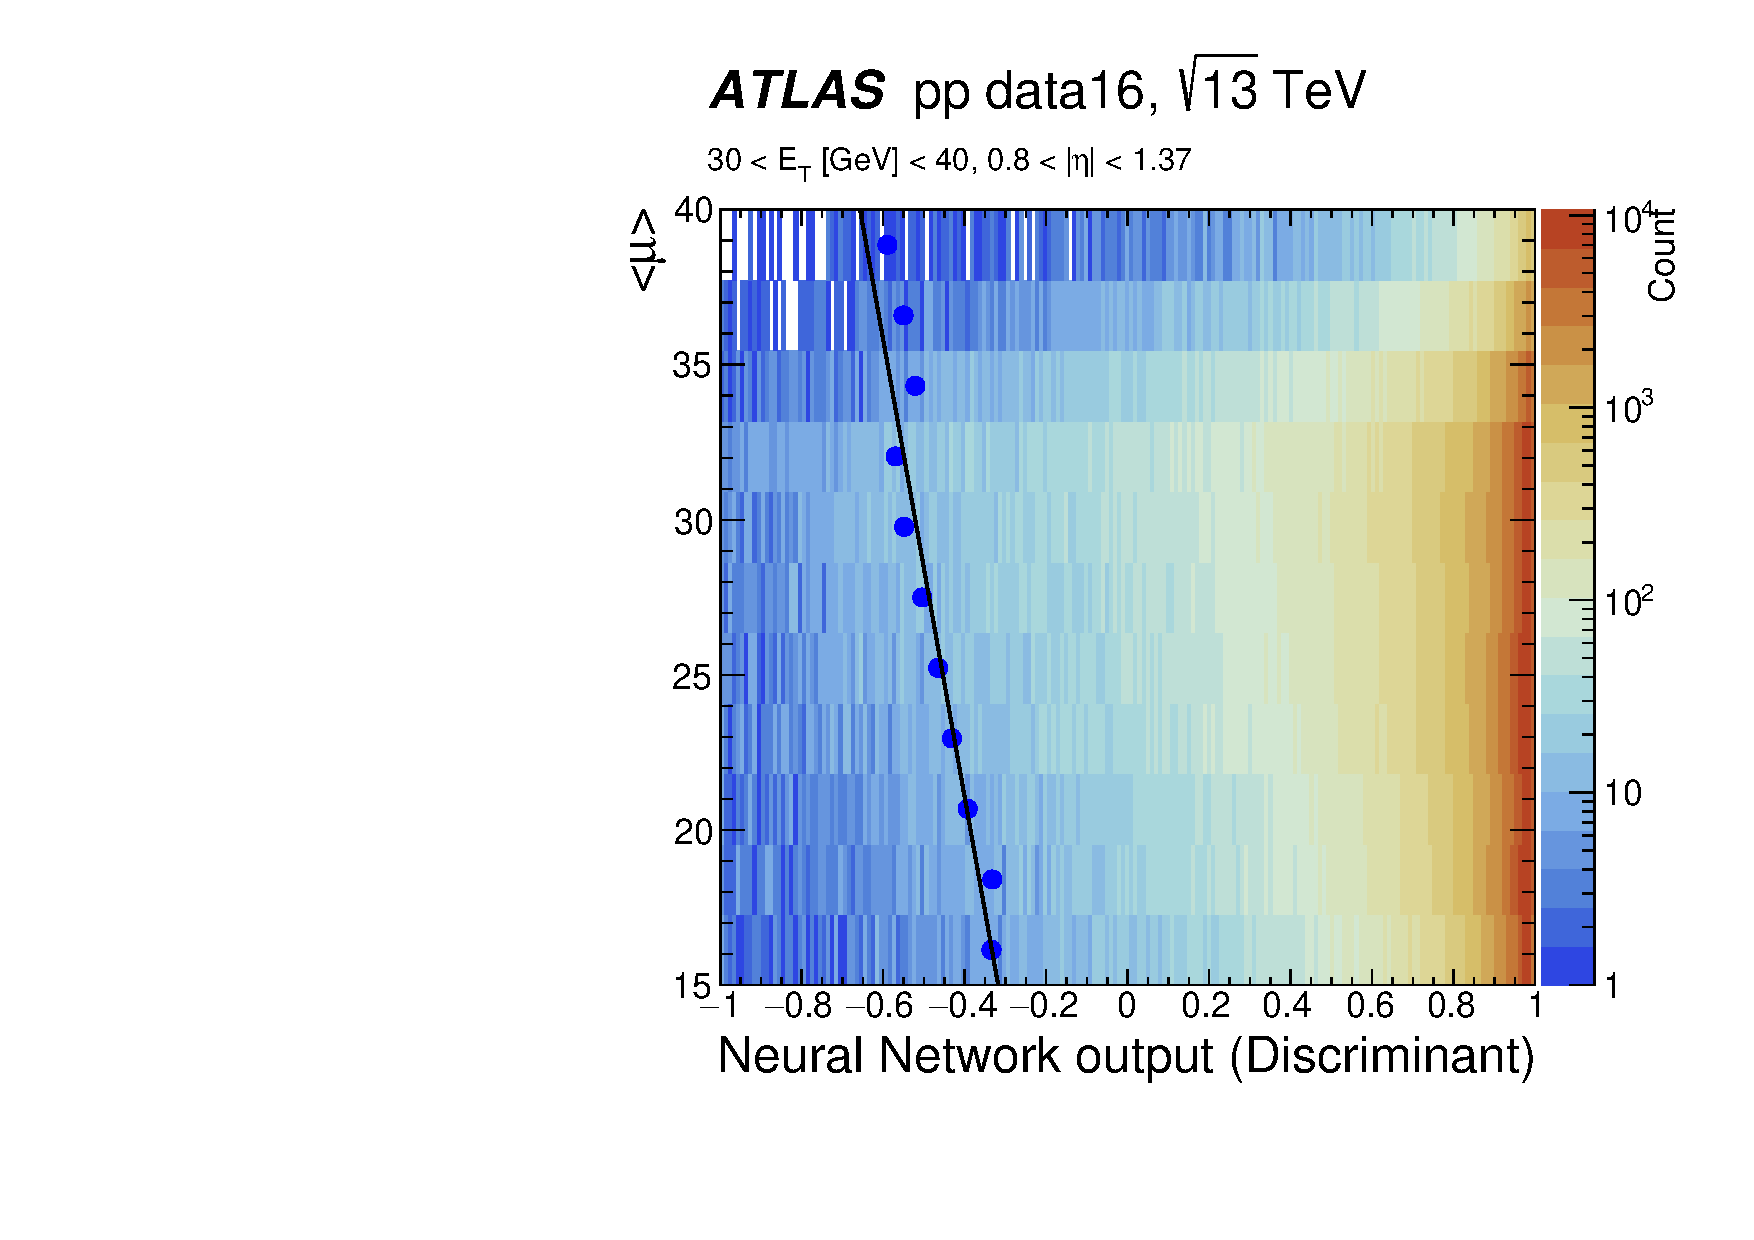
\includegraphics[width=\textwidth]{sections/02_ringer/figures/nn_output_versus_mu_with_tanh.pdf}
  \caption{MLP output with \DIFaddbeginFL \DIFaddFL{a }\DIFaddendFL hyperbolic tangent \DIFdelbeginFL \DIFdelFL{as }\DIFdelendFL activation function in the output neuron \DIFdelbeginFL \DIFdelFL{w.r.t }\DIFdelendFL \DIFaddbeginFL \DIFaddFL{versus }\DIFaddendFL pile-up.}
  \label{fig:nn_correction_with_tansig}
  \end{subfigure}
  \hfill
  \begin{subfigure}[c]{.48\textwidth}
  \centering
  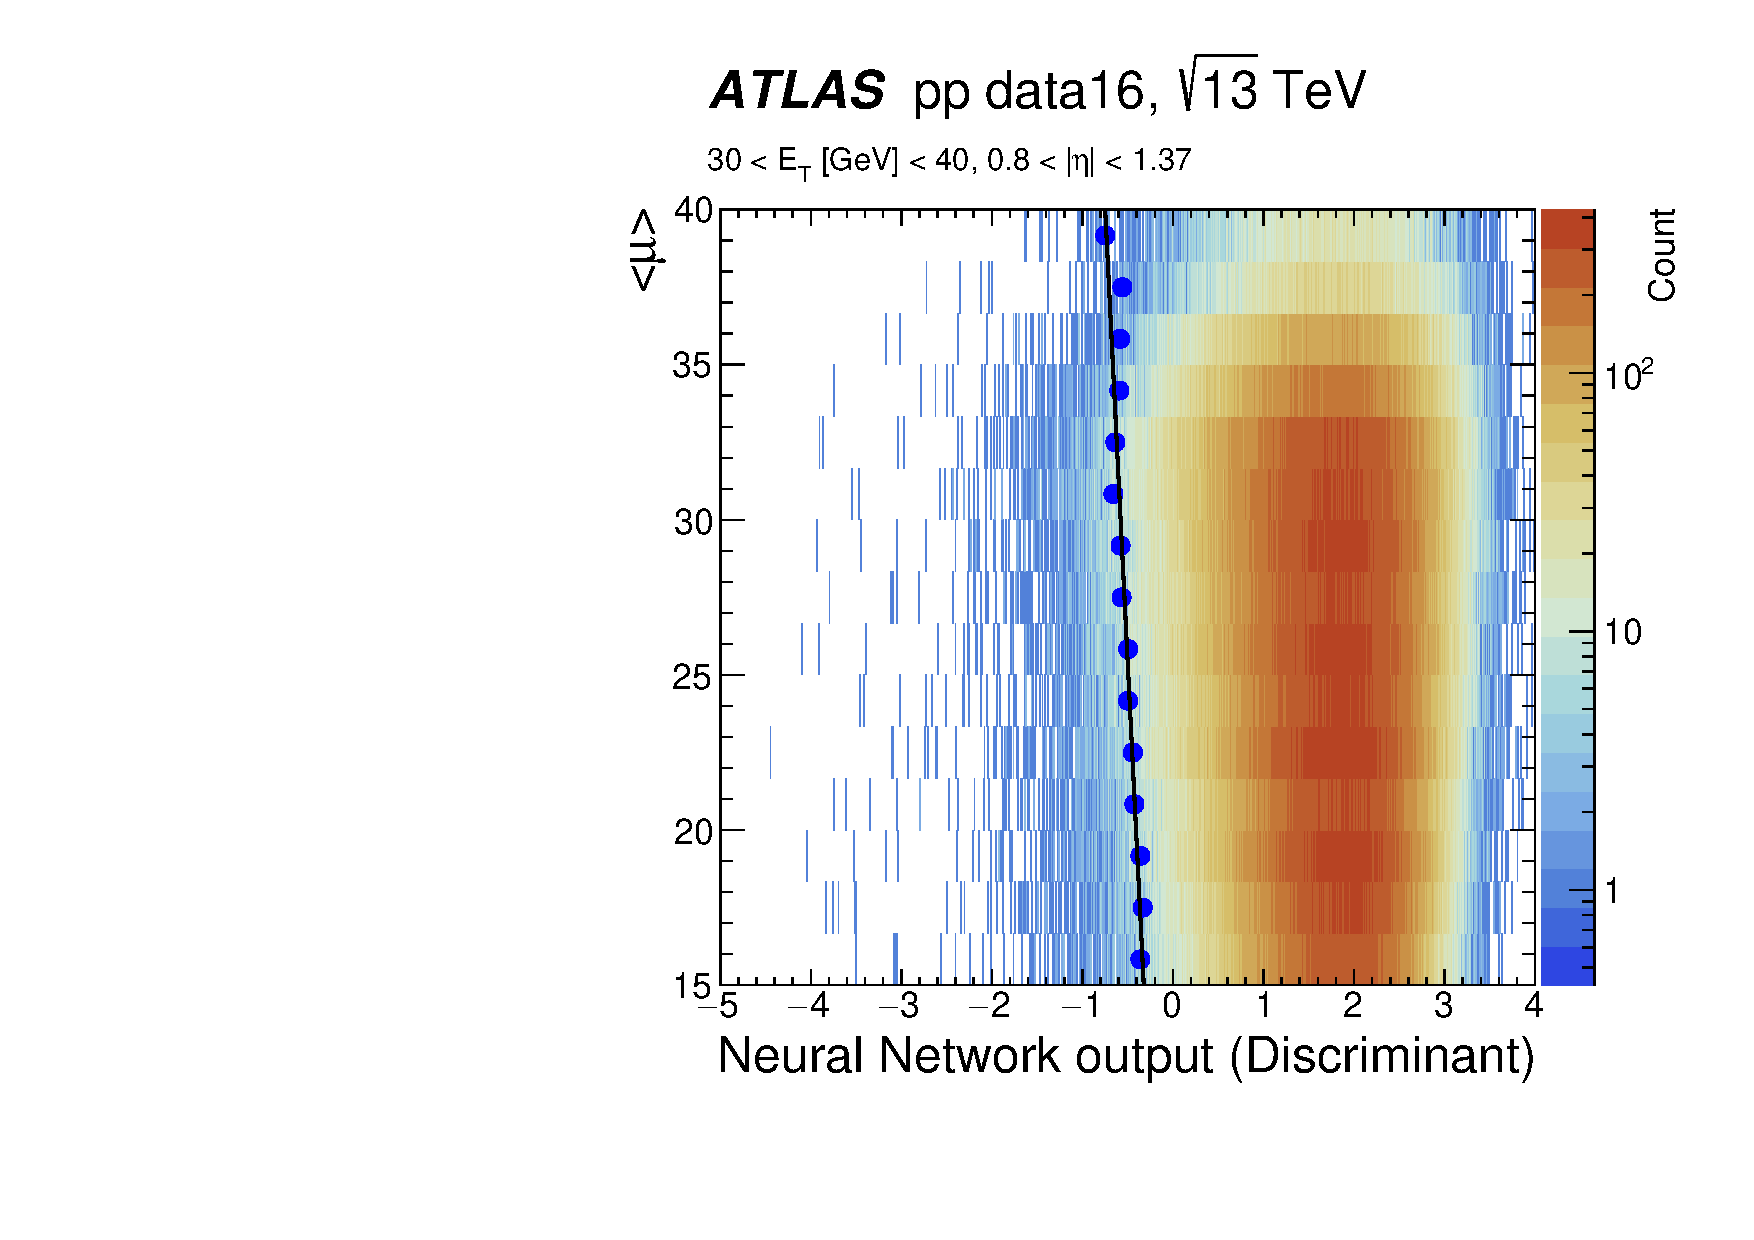
\includegraphics[width=\textwidth]{sections/02_ringer/figures/nn_output_versus_mu.pdf}
  \caption{MLP output with \DIFaddbeginFL \DIFaddFL{a }\DIFaddendFL linear \DIFdelbeginFL \DIFdelFL{as }\DIFdelendFL activation function in the output neuron \DIFdelbeginFL \DIFdelFL{w.r.t }\DIFdelendFL \DIFaddbeginFL \DIFaddFL{versus }\DIFaddendFL pile-up.}
  \label{fig:nn_correction_without_tansig}
  \end{subfigure}
  %\hfill
  \caption{
    \rnn output as a function of \DIFdelbeginFL %DIFDELCMD < \avgmu{} %%%
\DIFdelendFL \DIFaddbeginFL \DIFaddFL{pile-up, }\avgmu\DIFaddFL{, }\DIFaddendFL for $Z\rightarrow ee$ probes in 
    2016 collision data selected using the training criteria.
    The computed threshold per \avgmu{} unit for achieving the \DIFdelbeginFL \DIFdelFL{target 
    }\DIFdelendFL \DIFaddbeginFL \DIFaddFL{targeted 
    }\DIFaddendFL efficiency is shown \DIFdelbeginFL \DIFdelFL{in blue }\DIFdelendFL \DIFaddbeginFL \DIFaddFL{as a }\DIFaddendFL full \DIFaddbeginFL \DIFaddFL{blue }\DIFaddendFL circle. The black line is a linear fit \DIFdelbeginFL \DIFdelFL{of }\DIFdelendFL \DIFaddbeginFL \DIFaddFL{to }\DIFaddendFL the thresholds.
    The output space is computed using the trained model without modifications in (a), 
    while in (b) the activation function \DIFdelbeginFL \DIFdelFL{from }\DIFdelendFL \DIFaddbeginFL \DIFaddFL{in }\DIFaddendFL the output neuron is replaced \DIFdelbeginFL \DIFdelFL{by }\DIFdelendFL \DIFaddbeginFL \DIFaddFL{with }\DIFaddendFL a linear function.
  }%
  \end{center}
\end{figure}

\begin{figure}[!ht]
  \centering
  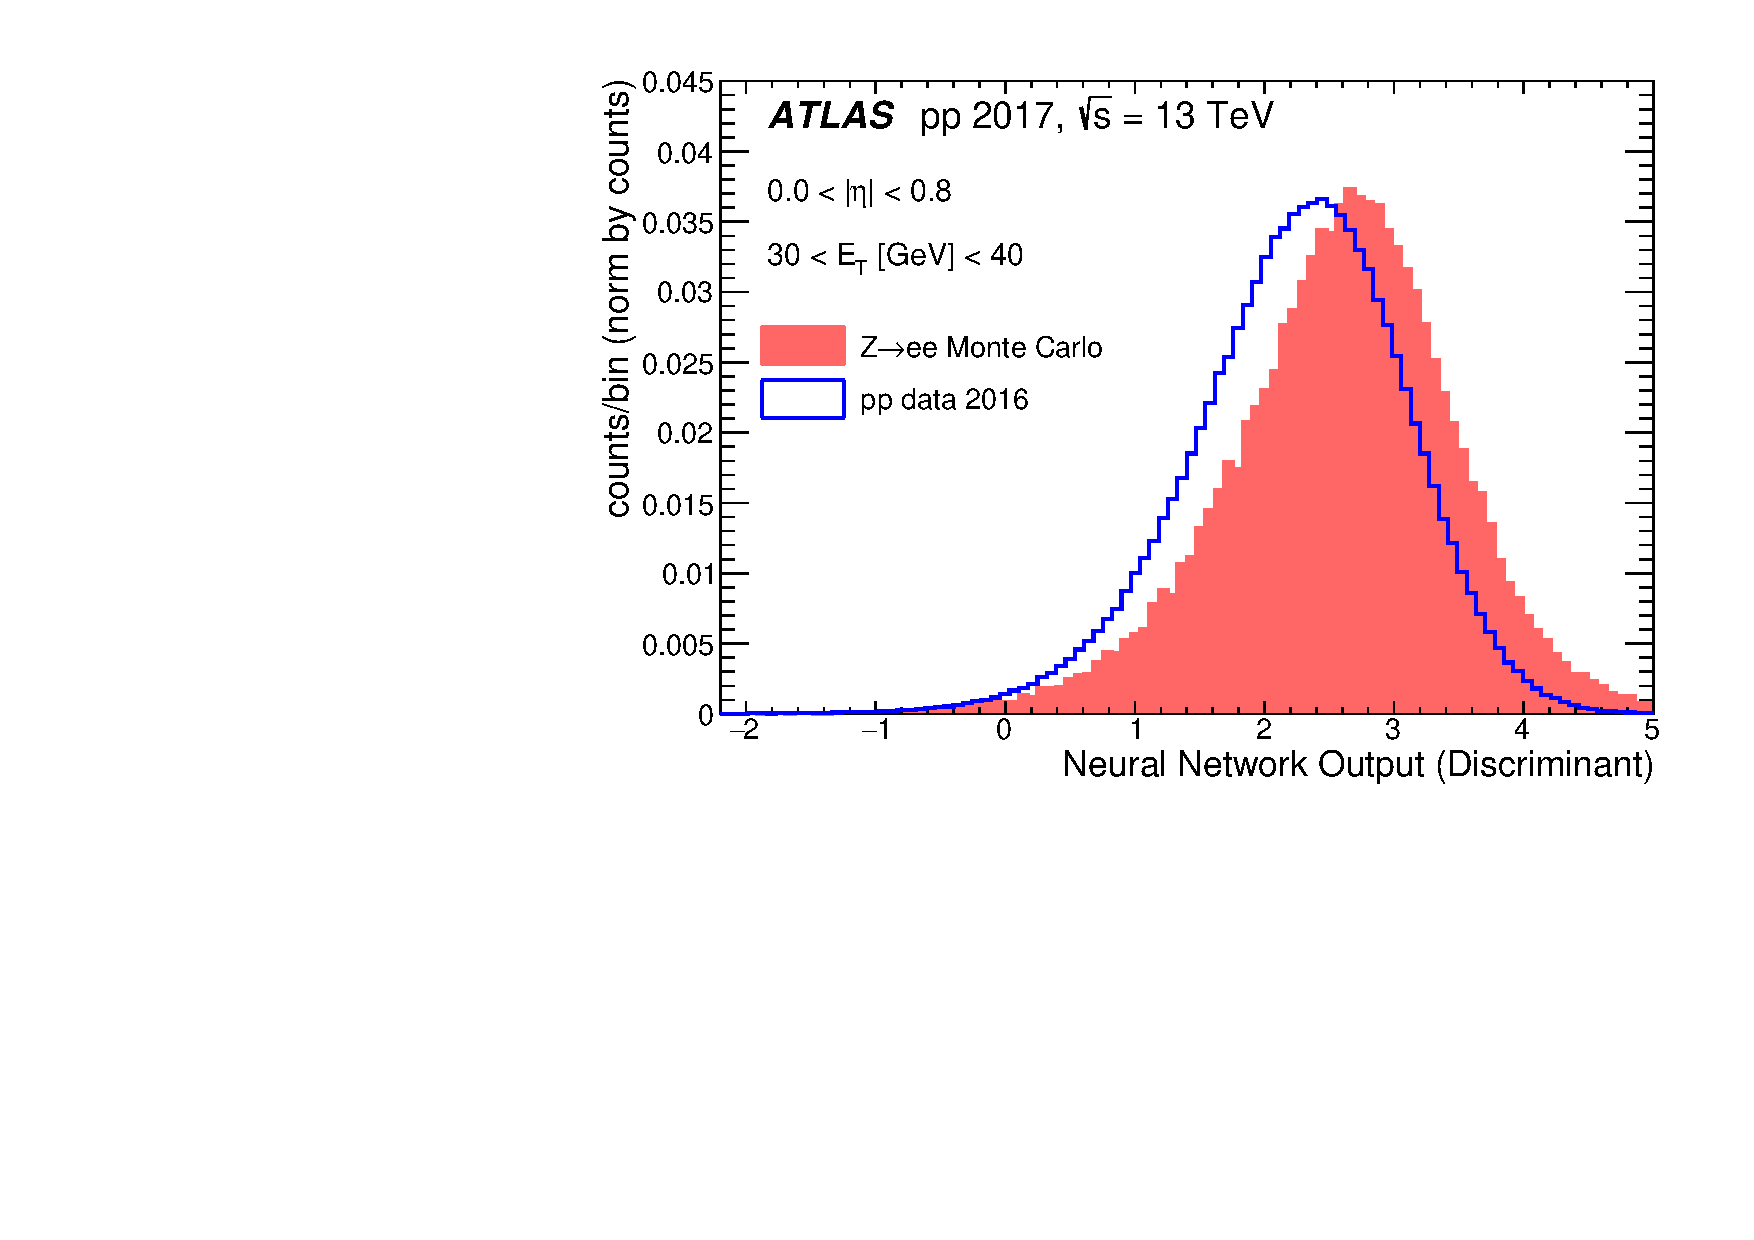
\includegraphics[width=0.7\textwidth]{sections/02_ringer/figures/nn_output_mc15_versus_data16_et2_eta0.pdf}
  \caption{Differences between simulation samples (red) and collision data (blue) obtained in 2016 for \DIFdelbeginFL \DIFdelFL{a }\DIFdelendFL \DIFaddbeginFL \DIFaddFL{one }\DIFaddendFL region of the phase space.
  The comparison is made between the normalized distributions \DIFdelbeginFL \DIFdelFL{obtained in both cases for }\DIFdelendFL \DIFaddbeginFL \DIFaddFL{of }\DIFaddendFL the output of the neural network (\DIFaddbeginFL \DIFaddFL{the }\DIFaddendFL discriminant) \DIFdelbeginFL \DIFdelFL{generated }\DIFdelendFL \DIFaddbeginFL \DIFaddFL{obtained }\DIFaddendFL for \DIFdelbeginFL \DIFdelFL{the samples present in the signal set within the selected region of the phase space}\DIFdelendFL \DIFaddbeginFL \DIFaddFL{these two cases}\DIFaddendFL . 
  The shift \DIFdelbeginFL \DIFdelFL{on the }\DIFdelendFL \DIFaddbeginFL \DIFaddFL{in }\DIFaddendFL discriminant \DIFdelbeginFL \DIFdelFL{generated by the neural network }\DIFdelendFL \DIFaddbeginFL \DIFaddFL{value }\DIFaddendFL between simulation and collision data is caused by \DIFdelbeginFL \DIFdelFL{the }\DIFdelendFL differences \DIFdelbeginFL \DIFdelFL{of }\DIFdelendFL \DIFaddbeginFL \DIFaddFL{between }\DIFaddendFL the \DIFdelbeginFL \DIFdelFL{simulation-data }\DIFdelendFL \DIFaddbeginFL \DIFaddFL{simulation and data }\DIFaddendFL rings used as input
  \DIFdelbeginFL \DIFdelFL{into }\DIFdelendFL \DIFaddbeginFL \DIFaddFL{to }\DIFaddendFL the model. }
  \label{fig:nn_mc15_vs_data16}
\end{figure}


\DIFdelbegin \DIFdel{Furthermore, it }\DIFdelend \DIFaddbegin \DIFadd{It }\DIFaddend was observed
that the rings in the region $2.37<\abseta<2.47$ had particular profiles due to
the lack of strip cells in this region and \DIFdelbegin \DIFdel{demanded }\DIFdelend \DIFaddbegin \DIFadd{required }\DIFaddend a specific discriminant \DIFdelbegin \DIFdel{requirement }\DIFdelend \DIFaddbegin \DIFadd{threshold }\DIFaddend in order to keep \DIFaddbegin \DIFadd{the }\DIFaddend signal efficiencies close to \DIFaddbegin \DIFadd{those of }\DIFaddend the cut-based triggers. In order to avoid retraining all models, it was decided to split the last $|\eta|$ region in two, from $1.37\rightarrow 2.5$ to $1.37\rightarrow2.37\rightarrow2.5$, and duplicate all models, for this region, to the new bin. Finally, the set used to \DIFdelbegin \DIFdel{operated }\DIFdelend \DIFaddbegin \DIFadd{operate }\DIFaddend in 2017, which \DIFdelbegin \DIFdel{is a combination of }\DIFdelend \DIFaddbegin \DIFadd{combines }\DIFaddend every $\eta$ boundary with each \DIFdelbegin \DIFdel{$E_T$ }\DIFdelend \DIFaddbegin \ET \DIFaddend boundary, has a total of 25 MLP models. The set\DIFaddbegin \DIFadd{'s }\DIFaddend boundaries are defined \DIFdelbegin \DIFdel{by }\DIFdelend \DIFaddbegin \DIFadd{in }\DIFaddend Table~\ref{tab:ensemble_regions}.



\begin{table}[htb]
\begin{center}
	{\DIFaddbeginFL \caption{\ET \DIFaddFL{and $\eta$ boundaries used to create the set of neural networks.}}
	\label{tab:ensemble_regions}
	\DIFaddendFL \small
	\begin{tabular}{cccc}
		\hline \hline
		\DIFdelbeginFL %DIFDELCMD < \multicolumn{4}{c}{Model Adjust}                                                                 %%%
\DIFdelendFL \DIFaddbeginFL \multicolumn{4}{c}{Model Adjustment}                                                                 \DIFaddendFL \\ \hline
		\DIFdelbeginFL %DIFDELCMD < \multicolumn{2}{c|}{$E_T$ {[}GeV{]} Boundaries} %%%
\DIFdelendFL \DIFaddbeginFL \multicolumn{2}{c|}{$\ET$ {[}GeV{]} boundaries} \DIFaddendFL & \DIFdelbeginFL %DIFDELCMD < \multicolumn{2}{l}{$|\eta|$ Boundaries}        %%%
\DIFdelendFL \DIFaddbeginFL \multicolumn{2}{l}{$|\eta|$ boundaries}        \DIFaddendFL \\ \hline
		\DIFdelbeginFL %DIFDELCMD < \multicolumn{2}{c|}{$15 \leq E_T < 20 $}        %%%
\DIFdelendFL \DIFaddbeginFL \multicolumn{2}{c|}{$15 \leq \ET < 20 $}        \DIFaddendFL & \multicolumn{2}{l}{$0.00 \leq |\eta| < 0.80 $}   \\
		\DIFdelbeginFL %DIFDELCMD < \multicolumn{2}{c|}{$20 \leq E_T < 30 $}        %%%
\DIFdelendFL \DIFaddbeginFL \multicolumn{2}{c|}{$20 \leq \ET < 30 $}        \DIFaddendFL & \multicolumn{2}{l}{$0.80 \leq |\eta| < 1.37 $}  \\
		\DIFdelbeginFL %DIFDELCMD < \multicolumn{2}{c|}{$30 \leq E_T < 40 $}        %%%
\DIFdelendFL \DIFaddbeginFL \multicolumn{2}{c|}{$30 \leq \ET < 40 $}        \DIFaddendFL & \multicolumn{2}{l}{$1.37 \leq |\eta| < 1.54 $} \\
		\DIFdelbeginFL %DIFDELCMD < \multicolumn{2}{c|}{$40 \leq E_T < 50 $}        %%%
\DIFdelendFL \DIFaddbeginFL \multicolumn{2}{c|}{$40 \leq \ET < 50 $}        \DIFaddendFL & \multicolumn{2}{l}{$1.54 \leq |\eta| < 2.37 $} \\
		\DIFdelbeginFL %DIFDELCMD < \multicolumn{2}{c|}{$E_T \geq 50 $}    %%%
\DIFdelendFL \DIFaddbeginFL \multicolumn{2}{c|}{~~~~~~~~~$\ET \geq 50 $}    \DIFaddendFL & \multicolumn{2}{l}{$2.37 \leq |\eta| < 2.47 $} \\ \hline \hline
	\end{tabular}
}
\end{center}
\DIFdelbeginFL %DIFDELCMD < \caption{%
{%DIFAUXCMD
\DIFdelFL{$E_T$ and $\eta$ boundaries used to create the set of neural networks.}}
%DIFAUXCMD
%DIFDELCMD < \label{tab:ensemble_regions}
%DIFDELCMD < %%%
\DIFdelendFL \end{table}

On the other hand, the 2018 training procedure employed a single set structure for all working points and used the 2017 collision data, selected with  \Zee{} \tnp{} event selection, for training, as was the case for the derivation of \DIFaddbegin \DIFadd{the }\DIFaddend offline and final \hlt likelihood models~\cite{PERF-2017-01}. 
Most of the procedure was kept unchanged for 2018. The developments for 2018 data benefited from the \DIFdelbegin \DIFdel{similarity of data conditions with respect to }\DIFdelend \DIFaddbegin \DIFadd{data conditions being similar to those in }\DIFaddend 2017. To simplify the training strategy, the selection of three models for each training was abandoned, keeping only the \spmax{} model, as the previous approach was more complex without a clear \DIFdelbegin \DIFdel{return on }\DIFdelend \DIFaddbegin \DIFadd{increase in }\DIFaddend trigger efficiency. 

Likewise, MLPs with 5 to 10 units in the hidden layer were tuned, as most models did not require more than 10 units in 2017. The training optimizer was changed to \DIFdelbegin \DIFdel{the }\DIFdelend \emph{Adam}~\cite{kingma2014adam}, instead \DIFaddbegin \DIFadd{of }\DIFaddend RPROP, and the MLP model topology was modified to \DIFdelbegin \DIFdel{: }\DIFdelend \DIFaddbegin \DIFadd{have }\DIFaddend a hidden layer with \DIFdelbegin \DIFdel{a }\DIFdelend fully connected neurons\DIFdelbegin \DIFdel{with a }\DIFdelend \DIFaddbegin \DIFadd{, with }\DIFaddend rectified linear units (RELU) as the activation function\DIFaddbegin \DIFadd{, }\DIFaddend and an output layer with one neuron using \DIFdelbegin \DIFdel{the sigmoid as the }\DIFdelend \DIFaddbegin \DIFadd{a sigmoid }\DIFaddend activation function. With a larger time span for entering operation, specialized MLPs \DIFaddbegin \DIFadd{were implemented }\DIFaddend in the region \DIFdelbegin \DIFdel{where a change was detected in the ring profiles }\DIFdelend \DIFaddbegin \DIFadd{$2.37<\abseta<2.47$, where different ring profiles were observed }\DIFaddend before 2017 operation\DIFdelbegin \DIFdel{between $2.37<\abseta<2.47$ was added}\DIFdelend , resulting in the operation of \SI{25}{MLPs}. Finally, the \DIFdelbegin \DIFdel{correction limit }\DIFdelend \DIFaddbegin \DIFadd{upper bound for threshold corrections }\DIFaddend was set to $\avgmu{}=100$~\DIFdelbegin \DIFdel{collisions in other }\DIFdelend \DIFaddbegin \DIFadd{pile-up interactions in order }\DIFaddend to extrapolate the operation of the models to a \DIFdelbegin \DIFdel{never reached }\DIFdelend \DIFaddbegin \DIFadd{never-reached }\DIFaddend pile-up level\DIFdelbegin \DIFdel{condition}\DIFdelend . 





 \newpage  % 
 \newpage \section{Online \DIFdelbegin \DIFdel{Deployment }\DIFdelend \DIFaddbegin \DIFadd{deployment }\DIFaddend and \DIFdelbegin \DIFdel{Performance}\DIFdelend \DIFaddbegin \DIFadd{performance}\DIFaddend }%
\label{sec:operation}


 \DIFdelbegin \DIFdel{During 2017-2018 years (LHC Run 2), the actual }\DIFdelend \DIFaddbegin \DIFadd{The }\DIFaddend \rnn{} \DIFdelbegin \DIFdel{implementation has made in four chronological stages }\DIFdelend \DIFaddbegin \DIFadd{algorithm was implemented in four stages during 2017--2018 in LHC }\RunTwo\DIFaddend :

\begin{enumerate}[i]
  \item A development stage up to early 2017, where the \rnn{}\DIFaddbegin \DIFadd{'s
      }\DIFaddend potential was estimated from trigger emulation and data reprocessing\DIFdelbegin \DIFdel{;
  }\DIFdelend \DIFaddbegin \DIFadd{.
  }\DIFaddend \item The commissioning stage \DIFdelbegin \DIFdel{(}%DIFDELCMD < \SI{5.4}{\per\femto\barn}%%%
\DIFdel{) occurred }\DIFdelend in
      early 2017 runs \DIFaddbegin \DIFadd{($5.4~\ifb$}}\DIFadd{)}\DIFaddend , where all primary
      triggers were duplicated \DIFdelbegin \DIFdel{with }\DIFdelend \DIFaddbegin \DIFadd{and }\DIFaddend either the \rnn{} or cut-based \DIFdelbegin \DIFdel{algorithms
      operating }\DIFdelend \DIFaddbegin \DIFadd{algorithm
      operated }\DIFaddend in the \fastcalo{} stage of the HLT\DIFdelbegin \DIFdel{;
   }\DIFdelend \DIFaddbegin \DIFadd{.
   }\DIFaddend \item The \DIFdelbegin \DIFdel{Operation }\DIFdelend \DIFaddbegin \DIFadd{operation }\DIFaddend stage, starting after \DIFdelbegin \DIFdel{2017 Technical Stop}\DIFdelend \DIFaddbegin \DIFadd{Technical Stop~}\DIFaddend 1 (TS1) \DIFdelbegin \DIFdel{. Triggers with }\DIFdelend \DIFaddbegin \DIFadd{in 2017. Triggers employing the }\DIFaddend \rnn{} \DIFdelbegin \DIFdel{are used as }\DIFdelend \DIFaddbegin \DIFadd{were used as the }\DIFaddend main triggers, and \DIFdelbegin \DIFdel{cut based are }\DIFdelend \DIFaddbegin \DIFadd{cut-based triggers were }\DIFaddend kept as backup triggers. Final validation of \DIFaddbegin \DIFadd{the }\DIFaddend \rnn{} \DIFdelbegin \DIFdel{is performed comparing data on }\DIFdelend \DIFaddbegin \DIFadd{was performed by comparing data from }\DIFaddend this period (\DIFdelbegin %DIFDELCMD < \SI{39.0}{\per\femto\barn}%%%
\DIFdelend \DIFaddbegin \DIFadd{$39.0~\ifb$}\DIFaddend ) as shown in Section~\ref{ssec:2017_ringer_operation} and Section~\ref{sec:off_ana}.
    \item \DIFaddbegin \DIFadd{The }\DIFaddend \rnn{}-only stage, during 2018. Duplicated cut-based triggers \DIFdelbegin \DIFdel{are }\DIFdelend \DIFaddbegin \DIFadd{were }\DIFaddend removed. The performance of the Neural-Ringer in 2018 is presented in Section~\ref{ssec:2018_ringer_operation}.

\end{enumerate}

This section reports the \rnn{}\DIFaddbegin \DIFadd{'s }\DIFaddend operation in each \DIFdelbegin \DIFdel{one }\DIFdelend of these periods. \DIFdelbegin \DIFdel{Additionally, a discussion about CPU time will be covered }\DIFdelend \DIFaddbegin \DIFadd{In addition, CPU-time usage is discussed }\DIFaddend in Section~\ref{ssec:cpu_reduction}.

\subsection{2017 \DIFdelbegin \DIFdel{Operation}\DIFdelend \DIFaddbegin \DIFadd{operation}\DIFaddend }\label{ssec:2017_ringer_operation}

A backup \DIFdelbegin \DIFdel{single electron }\DIFdelend \DIFaddbegin \DIFadd{single-electron }\DIFaddend HLT\_e28\_lhtight\_nod0\_(noringer)\_ivarloose trigger\DIFaddbegin \DIFadd{, both
 }\DIFaddend with and without (noringer) the \rnn{}\DIFaddbegin \DIFadd{, }\DIFaddend was employed for monitoring purposes after the first technical stop (TS1).
This trigger \DIFdelbegin \DIFdel{require }\DIFdelend \DIFaddbegin \DIFadd{requires }\DIFaddend an electron candidate with \DIFdelbegin \DIFdel{$E_T > 28$ }\DIFdelend \DIFaddbegin \DIFadd{$\ET > 28$~}\DIFaddend GeV satisfying the \DIFdelbegin \DIFdel{tight }\DIFdelend \DIFaddbegin \enquote{tight} \DIFaddend selection (lhtight\_nod0) with \DIFdelbegin \DIFdel{a loose }\DIFdelend \DIFaddbegin \enquote{loose} \DIFaddend isolation criteria (ivarloose)~\cite{TRIG-2018-05}. 
During the monitoring process, \DIFdelbegin \DIFdel{a similar operation of both triggers was observed }\DIFdelend \DIFaddbegin \DIFadd{the two trigger variants were observed to operate similarly }\DIFaddend in terms of signal efficiency \DIFdelbegin \DIFdel{using }\DIFdelend \DIFaddbegin \DIFadd{for }\DIFaddend the integrated luminosity \DIFdelbegin \DIFdel{along }\DIFdelend \DIFaddbegin \DIFadd{during }\DIFaddend the period, as shown in Figure~\ref{fig:2017_e28_after_ts1}. 
The trigger turn-on curves exhibit similar \DIFdelbegin \DIFdel{profile. In $\eta$, the }\DIFdelend \DIFaddbegin \ET \DIFadd{profiles. The }\DIFaddend \rnn{} shows a reasonably symmetric profile \DIFdelbegin \DIFdel{with respect to }\DIFdelend \DIFaddbegin \DIFadd{for }\DIFaddend positive and negative $\eta$ \DIFaddbegin \DIFadd{values}\DIFaddend . In addition, \DIFdelbegin \DIFdel{a }\DIFdelend \DIFaddbegin \DIFadd{an efficiency }\DIFaddend difference of about \DIFdelbegin \DIFdel{half to one percentage point may }\DIFdelend \DIFaddbegin \DIFadd{0.5\% to 1\% can }\DIFaddend be observed in \DIFdelbegin \DIFdel{$\eta$ because of }\DIFdelend the transition region \DIFdelbegin \DIFdel{between the end-cap }\DIFdelend \DIFaddbegin \DIFadd{near $|\eta| = 1.5$ between the endcaps }\DIFaddend and barrel. \DIFdelbegin \DIFdel{Besides aforementioned points, overall efficiency fluctuations are }\DIFdelend \DIFaddbegin \DIFadd{Apart from these features, the overall efficiency differences are typically }\DIFaddend smaller than a few\DIFdelbegin \DIFdel{per-mille}\DIFdelend \DIFaddbegin \DIFadd{~per~mille}\DIFaddend . Although a slightly more prominent efficiency loss \DIFdelbegin \DIFdel{with respect to }%DIFDELCMD < \avgmu{} %%%
\DIFdel{is observed }\DIFdelend \DIFaddbegin \DIFadd{is observed at large }\avgmu{} \DIFaddend in Figure~\ref{fig:e28_comp_mu} for the \rnn{} trigger, the electron efficiency was kept nearly the same. \DIFdelbegin \DIFdel{Such }\DIFdelend \DIFaddbegin \DIFadd{This }\DIFaddend loss occurs after the linear threshold correction limit of $\avgmu=40$ \DIFdelbegin \DIFdel{that }\DIFdelend was employed during 2017.

Other important triggers were assessed by comparing the trigger efficiencies \DIFdelbegin \DIFdel{on }\DIFdelend \DIFaddbegin \DIFadd{in }\DIFaddend 2017 collision data collected before and after switching to the \rnn{} algorithms\DIFdelbegin \DIFdel{can be observed }\DIFdelend \DIFaddbegin \DIFadd{, as shown }\DIFaddend in Figure~\ref{fig:2017_electron_triggers}. The \DIFdelbegin \DIFdel{single electron }\DIFdelend \DIFaddbegin \DIFadd{single-electron }\DIFaddend HLT\_e17\_lhvloose\_nod0\_L1EM15VHI trigger \DIFdelbegin \DIFdel{require }\DIFdelend \DIFaddbegin \DIFadd{requires }\DIFaddend an electron candidate \DIFaddbegin \DIFadd{with $\ET > 17$~GeV, }\DIFaddend seeded by the \DIFdelbegin \DIFdel{Level-1 }\DIFdelend \DIFaddbegin \DIFadd{first-level }\DIFaddend trigger L1\_EM15VHI\DIFdelbegin \DIFdel{with $E_T > 17$ GeV }\DIFdelend \DIFaddbegin \DIFadd{, and }\DIFaddend satisfying the loosest identification criteria (lhvloose). On the other hand, HLT\_e26\_lhtight\_nod0\_ivarloose \DIFdelbegin \DIFdel{and HLT\_e60\_lhmedium\_nod0 }\DIFdelend requires an electron candidate with \DIFdelbegin \DIFdel{$E_T>26$ Gev satisfying the tight }\DIFdelend \DIFaddbegin \DIFadd{$\ET>26$~GeV satisfying }\enquote{tight} \DIFaddend identification (lhtight) with \DIFdelbegin \DIFdel{loose }\DIFdelend \DIFaddbegin \enquote{loose} \DIFaddend isolation (ivarloose), and \DIFdelbegin \DIFdel{$E_T>60$ GeV satisfying the medium }\DIFdelend \DIFaddbegin \DIFadd{HLT\_e60\_lhmedium\_nod0 requires an electron candidate with $\ET>60$~GeV satisfying }\enquote{medium} \DIFaddend identification (lhmedium)\DIFdelbegin \DIFdel{, respectively. Here, the }\DIFdelend \DIFaddbegin \DIFadd{. The }\DIFaddend electron efficiency was also kept nearly unchanged for \DIFdelbegin \DIFdel{relevant single electron triggers. Note that results in this plot are computed with two different data taking periods: with or without}\DIFdelend \DIFaddbegin \DIFadd{these relevant single-electron triggers. As mentioned above, the results in Figure~\ref{fig:2017_electron_triggers} are computed for two different data-taking periods: one with, and the other without, }\DIFaddend the \rnn{} algorithm. 



\begin{figure}[h!tb]

  \begin{subfigure}[c]{.49\textwidth}
  \centering
  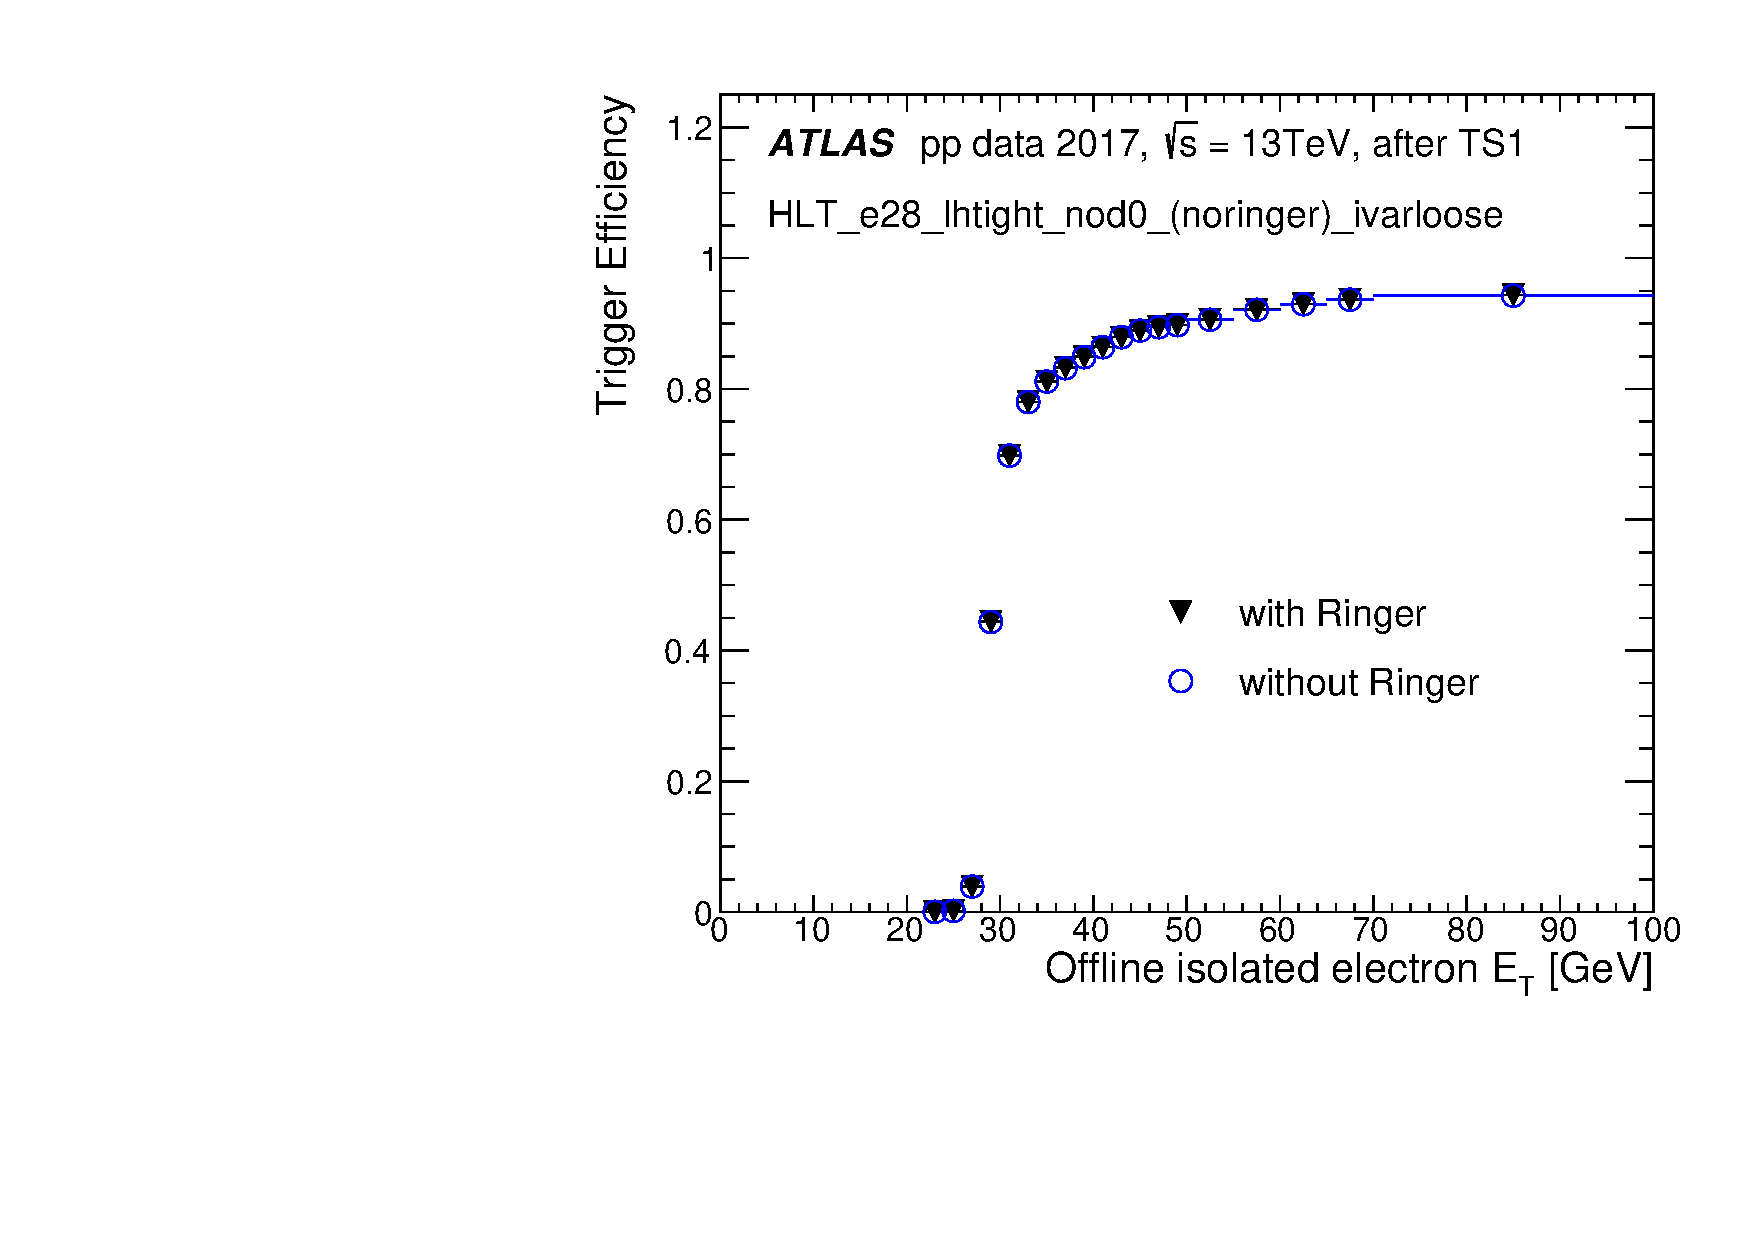
\includegraphics[width=\textwidth]{sections/03_operation/figures/efficiencies/eff_EGAM1_e28_ringer_and_noringer_2017_after_ts1_HLT_et.pdf}
  \caption{}
  \end{subfigure}
  %
  \begin{subfigure}[c]{.49\textwidth}
  \centering
  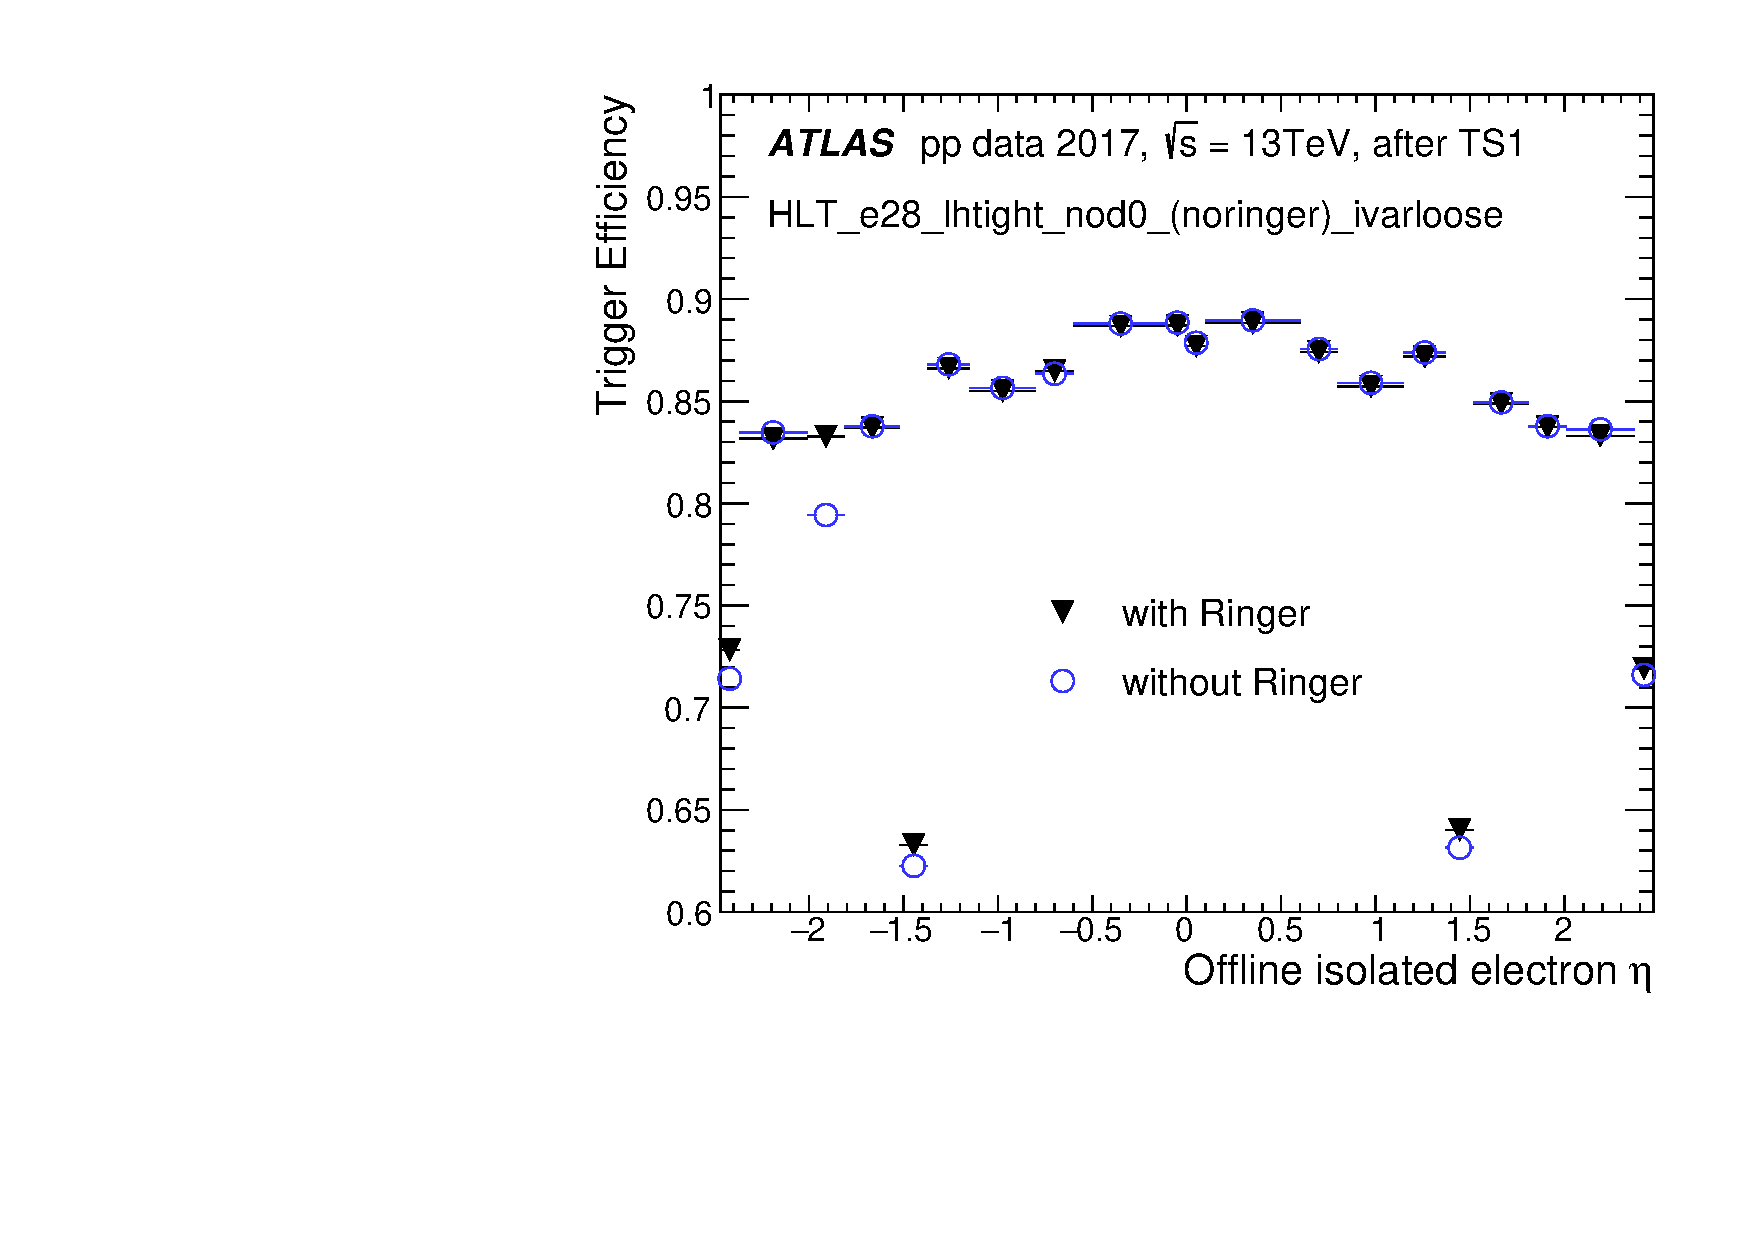
\includegraphics[width=\textwidth]{sections/03_operation/figures/efficiencies/eff_EGAM1_e28_ringer_and_noringer_2017_after_ts1_HLT_eta.pdf}
  \caption{}
  \end{subfigure}\\
  %
  \centering
  \begin{subfigure}[c]{.49\textwidth}
  \centering
  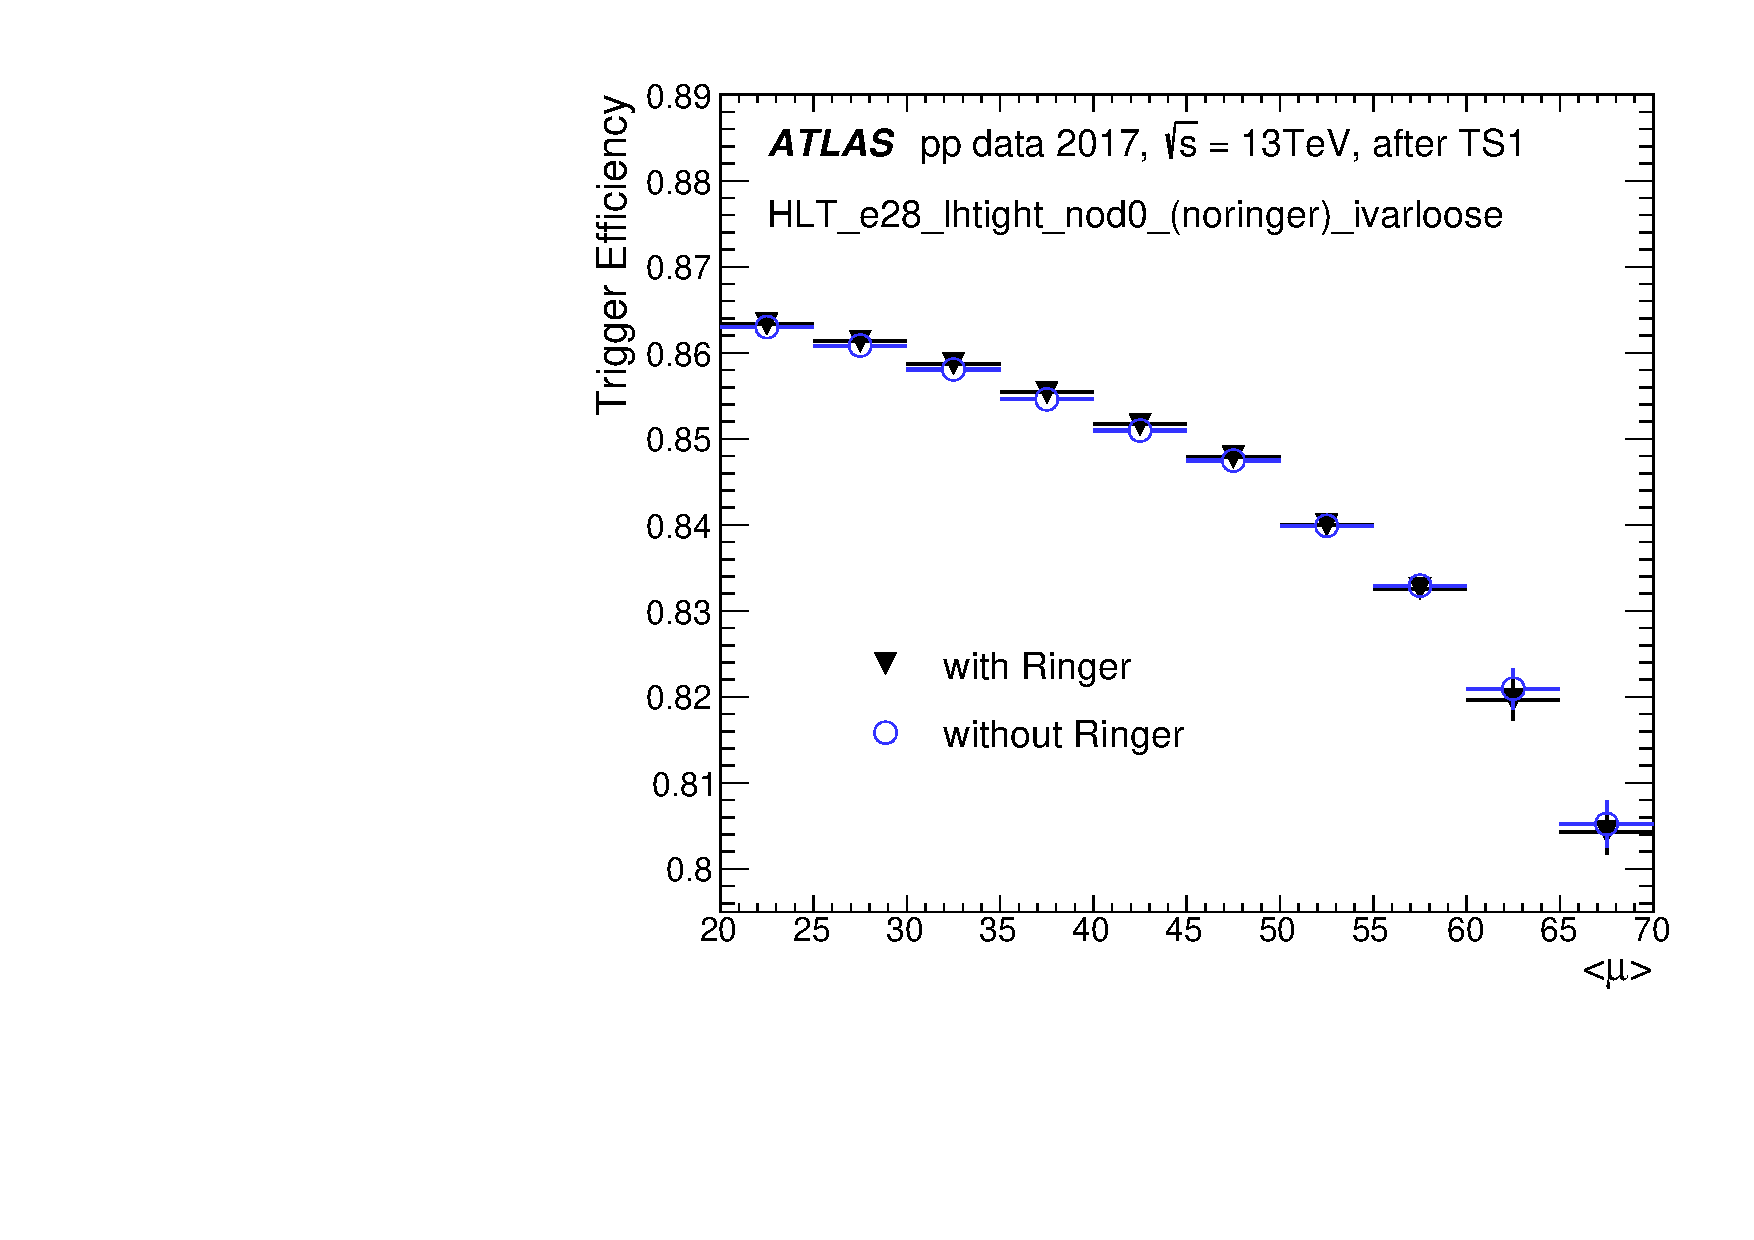
\includegraphics[width=\textwidth]{sections/03_operation/figures/efficiencies/eff_EGAM1_e28_ringer_and_noringer_2017_after_ts1_HLT_mu.pdf}
  \caption{}%
  \label{fig:e28_comp_mu}
  \end{subfigure}

  \caption{HLT electron efficiency \DIFaddbeginFL \DIFaddFL{in 2017 collision data }\DIFaddendFL as a function of \DIFdelbeginFL %DIFDELCMD < \et{} %%%
\DIFdelendFL (a) \DIFaddbeginFL \et{}\DIFaddendFL , \DIFdelbeginFL \DIFdelFL{\eta{} }\DIFdelendFL (\DIFdelbeginFL \DIFdelFL{c}\DIFdelendFL \DIFaddbeginFL \DIFaddFL{b}\DIFaddendFL ) \DIFaddbeginFL \DIFaddFL{\eta{}, }\DIFaddendFL and \DIFdelbeginFL %DIFDELCMD < \avgmu{} %%%
\DIFdelendFL (\DIFdelbeginFL \DIFdelFL{e}\DIFdelendFL \DIFaddbeginFL \DIFaddFL{c}\DIFaddendFL ) \DIFaddbeginFL \avgmu{} \DIFaddendFL for the \DIFdelbeginFL \DIFdelFL{single electron isolated }\DIFdelendFL \DIFaddbeginFL \DIFaddFL{single-isolated-electron }\DIFaddendFL trigger requiring $\et{} > \SI{28}{\GeV}$ and \DIFdelbeginFL \DIFdelFL{tight }\DIFdelendFL \DIFaddbeginFL \enquote{tight} \DIFaddendFL selection with and without the \rnn{} algorithm \DIFdelbeginFL \DIFdelFL{employing 2017 collision data }\DIFdelendFL after \DIFdelbeginFL \DIFdelFL{the }\DIFdelendFL \DIFaddbeginFL \DIFaddFL{its }\DIFaddendFL deployment.}
  \label{fig:2017_e28_after_ts1}
\end{figure}




\begin{figure}[h!tb]

 \begin{subfigure}[c]{.49\textwidth}
  \centering
  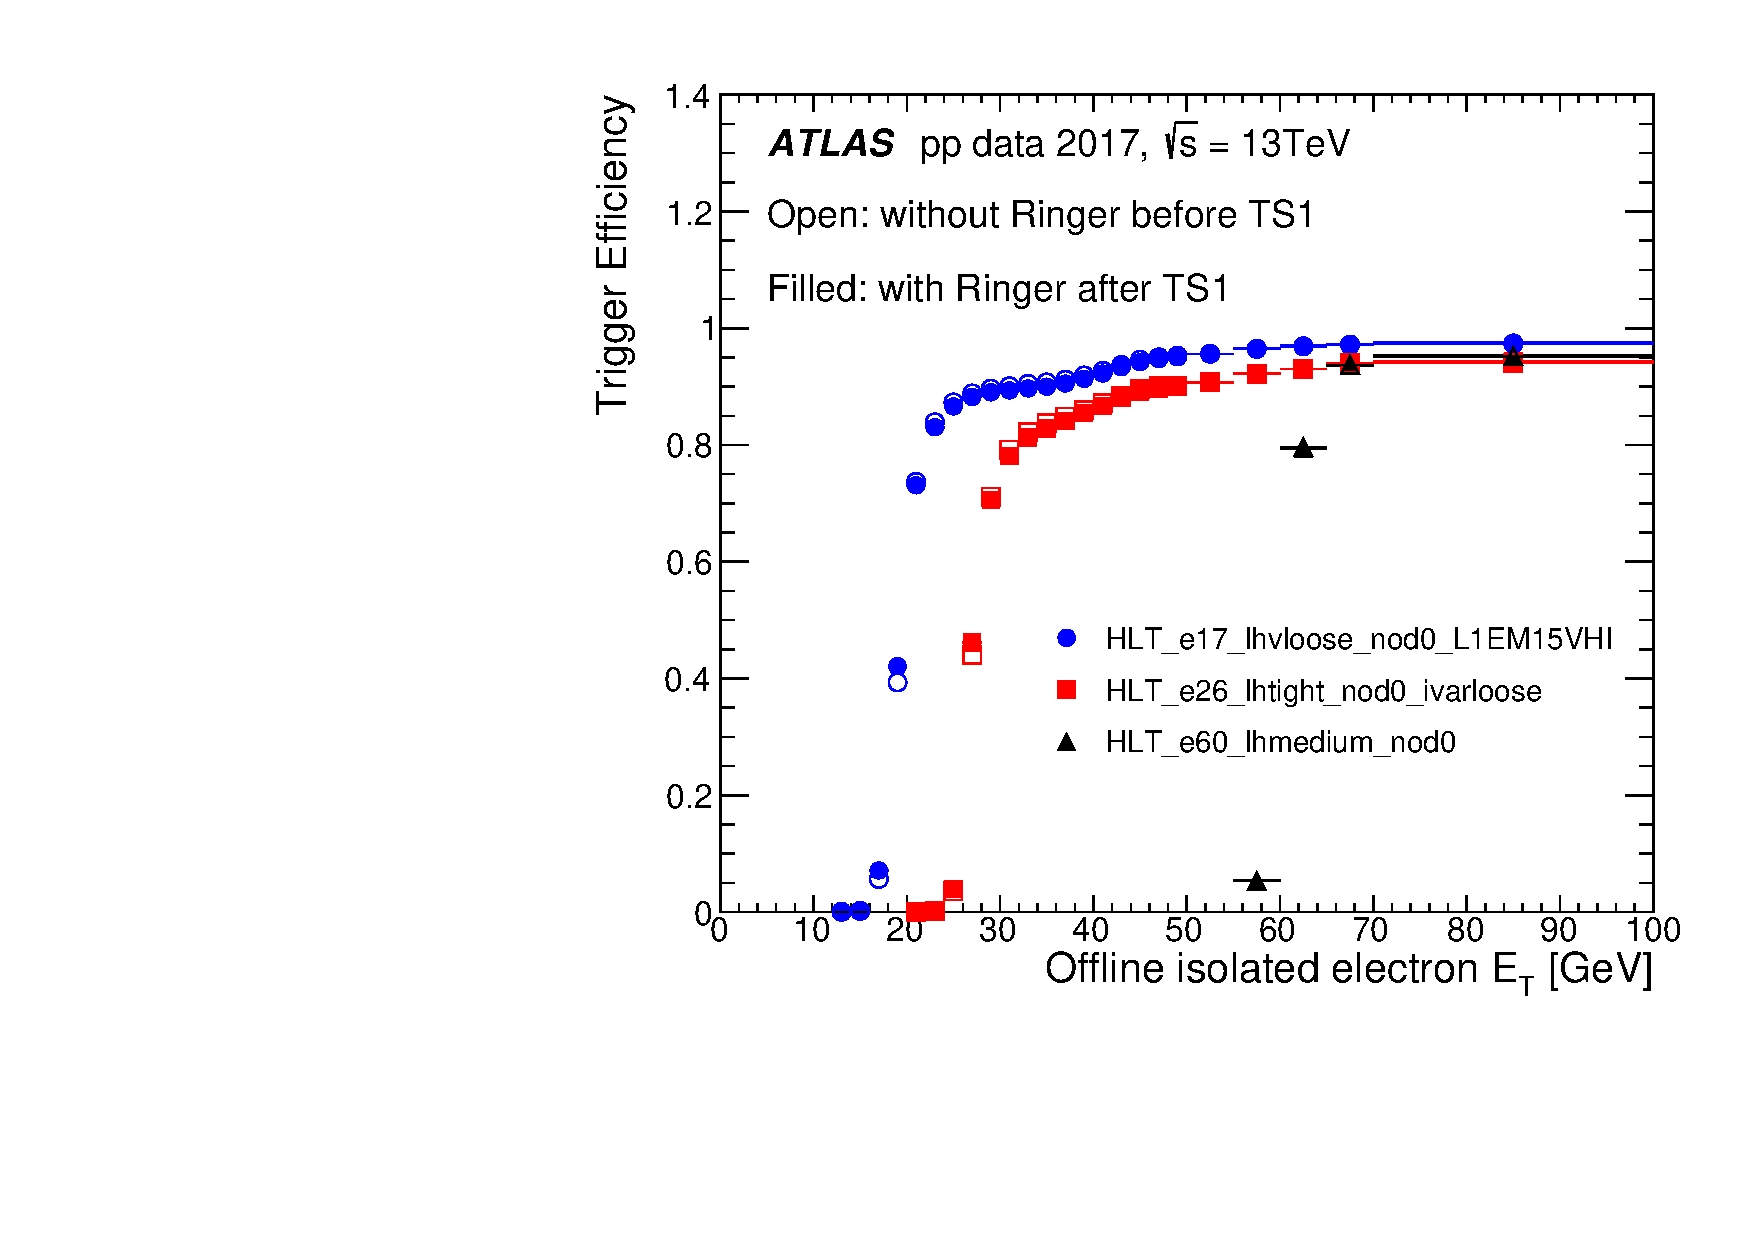
\includegraphics[width=\textwidth]{sections/03_operation/figures/efficiencies/eff_EGAM1_e17_e26_e60_2017_before_and_after_ts1_et.pdf}
  \caption{}%
  \end{subfigure}
  %
  \begin{subfigure}[c]{.49\textwidth}
  \centering
  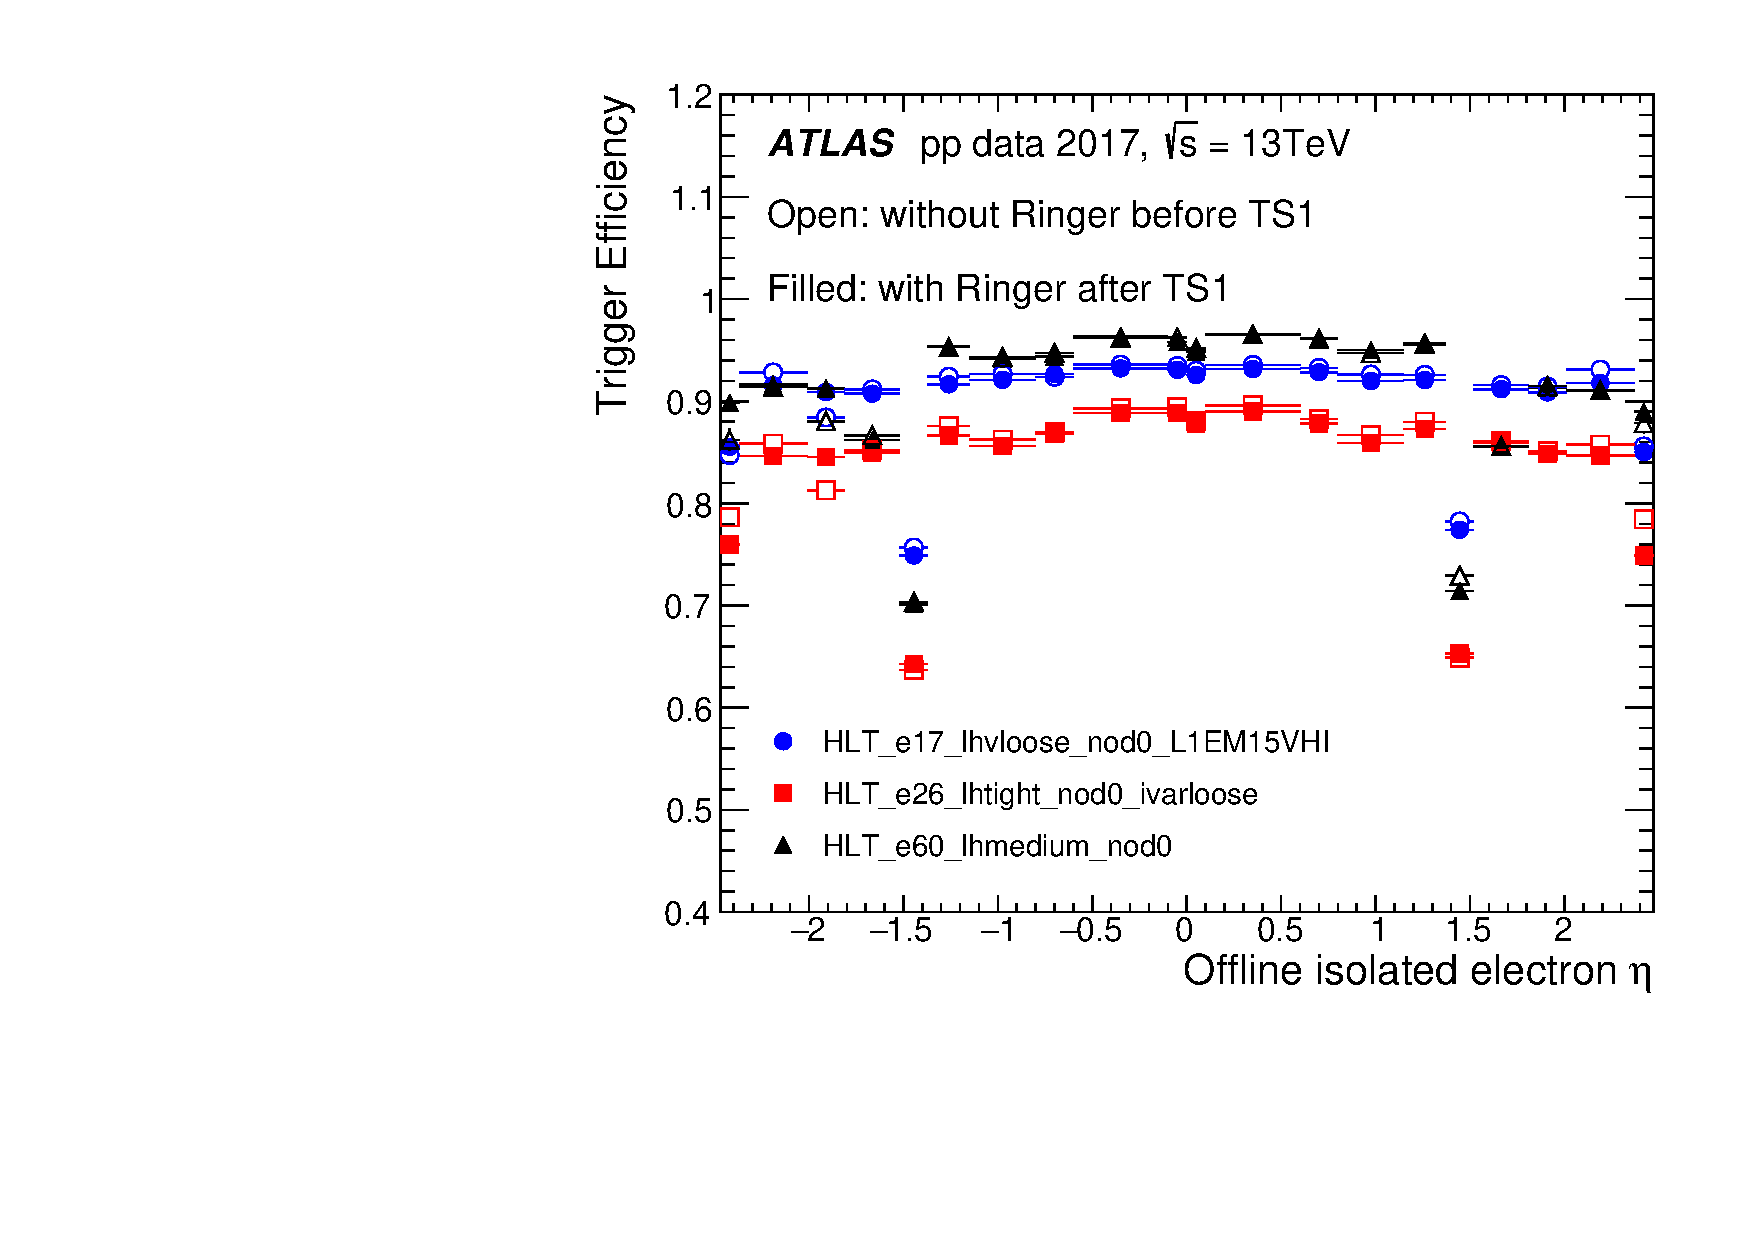
\includegraphics[width=\textwidth]{sections/03_operation/figures/efficiencies/eff_EGAM1_e17_e26_e60_2017_before_and_after_ts1_eta.pdf}
  \caption{}%
  \end{subfigure}

  \caption{
  Efficiency of three \DIFdelbeginFL \DIFdelFL{single electron }\DIFdelendFL \DIFaddbeginFL \DIFaddFL{single-electron }\DIFaddendFL triggers as a function of \DIFdelbeginFL %DIFDELCMD < \et %%%
\DIFdelendFL (a) \DIFaddbeginFL \et \DIFaddendFL and \DIFdelbeginFL \DIFdelFL{\eta }\DIFdelendFL (b) \DIFaddbeginFL \DIFaddFL{\eta }\DIFaddendFL for 2017 collision data. Open (filled) markers \DIFdelbeginFL \DIFdelFL{contain }\DIFdelendFL \DIFaddbeginFL \DIFaddFL{show }\DIFaddendFL the efficiency measurements \DIFdelbeginFL \DIFdelFL{on }\DIFdelendFL \DIFaddbeginFL \DIFaddFL{in }\DIFaddendFL runs before (after) the deployment of the \rnn{}, thus referring to triggers \DIFdelbeginFL \DIFdelFL{being }\DIFdelendFL executed without (with) the \rnn{} algorithm.}
  \label{fig:2017_electron_triggers}
\end{figure}




\DIFdelbegin \DIFdel{By contrasting the behavior }\DIFdelend \DIFaddbegin \DIFadd{The power of the }\rnn{} \DIFadd{algorithm is made clear by examining the behaviour }\DIFaddend of the duplicated trigger \DIFdelbegin \DIFdel{using fake electron collision data, it becomes clear the power of the }%DIFDELCMD < \rnn{} %%%
\DIFdel{algorithm. 
An overall reduction factor of
the fake rate }\DIFdelend \DIFaddbegin \DIFadd{for fake electron candidates in collision data. 
The overall fake-electron rate is reduced }\DIFaddend by a factor of 13.75 \DIFdelbegin \DIFdel{is achieved at }\DIFdelend \DIFaddbegin \DIFadd{at the }\DIFaddend \fastcalo step. It can be seen \DIFdelbegin \DIFdel{in }\DIFdelend \DIFaddbegin \DIFadd{on the left side of }\DIFaddend Figure~\ref{fig:2017_fake_triggers_after_ts1} \DIFdelbegin \DIFdel{left side, }\DIFdelend that the improvement at \DIFaddbegin \DIFadd{the }\DIFaddend \fastcalo \DIFaddbegin \DIFadd{step }\DIFaddend is similar for all
regions in the evaluated variables, \DIFaddbegin \DIFadd{which is }\DIFaddend particularly interesting when
considering the low \et{} and \DIFdelbegin \DIFdel{the end-cap }\DIFdelend \DIFaddbegin \DIFadd{endcap }\DIFaddend regions. Besides \DIFdelbegin \DIFdel{the capability of improving early fake rejection, the usage }\DIFdelend \DIFaddbegin \DIFadd{improving early fake-electron rejection, use }\DIFaddend of the \rnn{} also \DIFdelbegin \DIFdel{contributed to reduce the final fake rate at HLT
step
(}\DIFdelend \DIFaddbegin \DIFadd{resulted in a factor of two reduction in the final fake-electron rate from the HLT
(see right side of }\DIFaddend Figure~\ref{fig:2017_fake_triggers_after_ts1}\DIFdelbegin \DIFdel{right size)by a factor of 2}\DIFdelend \DIFaddbegin \DIFadd{)}\DIFaddend , mostly coming from the \DIFdelbegin \DIFdel{transition regions in the calorimeter}\DIFdelend \DIFaddbegin \DIFadd{calorimeter's barrel--endcap transition regions}\DIFaddend .


\begin{figure}[h!tb]
  \begin{subfigure}[c]{.49\textwidth}
  \centering
  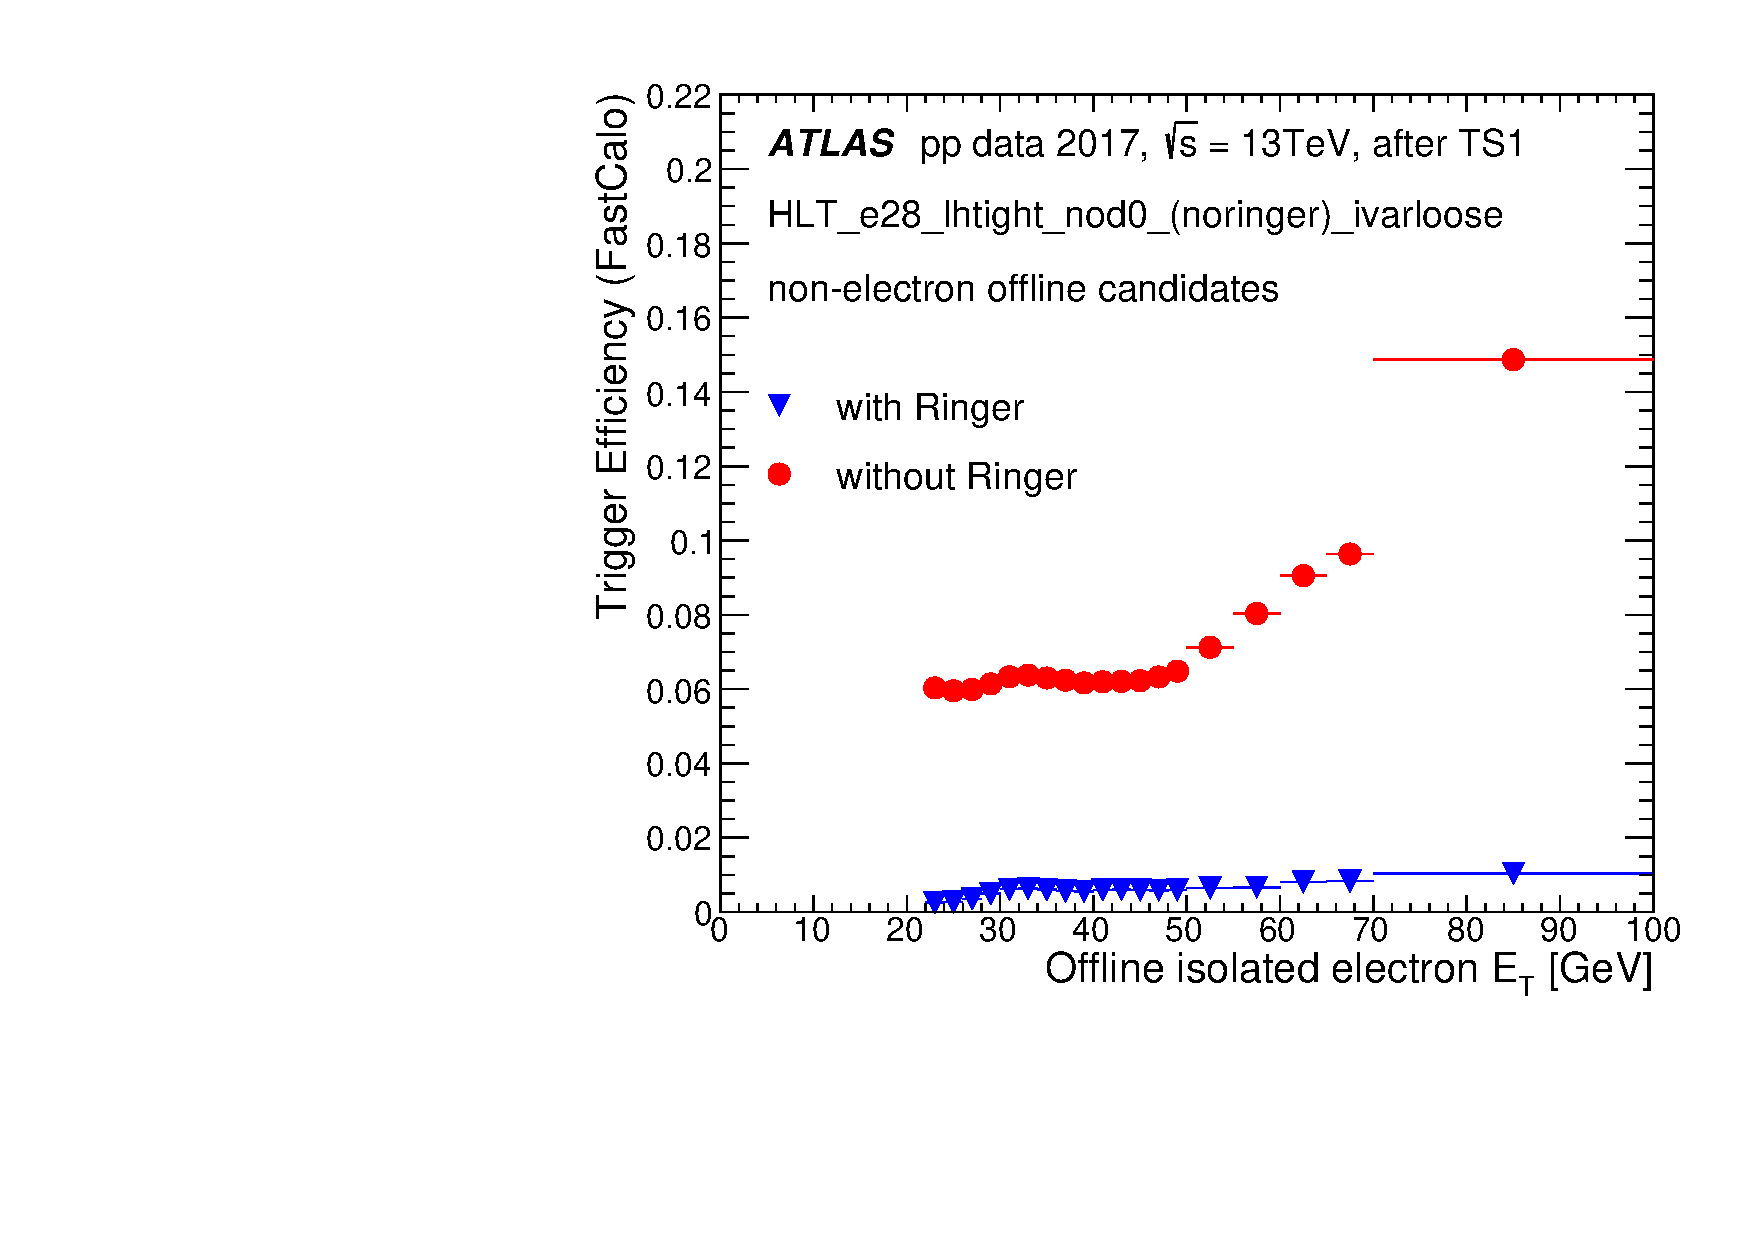
\includegraphics[width=\textwidth]{sections/03_operation/figures/efficiencies/eff_EGAM7_e28_ringer_and_noringer_2017_after_ts1_L2Calo_et.pdf}
  \caption{}
  \end{subfigure}
  %
  \begin{subfigure}[c]{.49\textwidth}
  \centering
  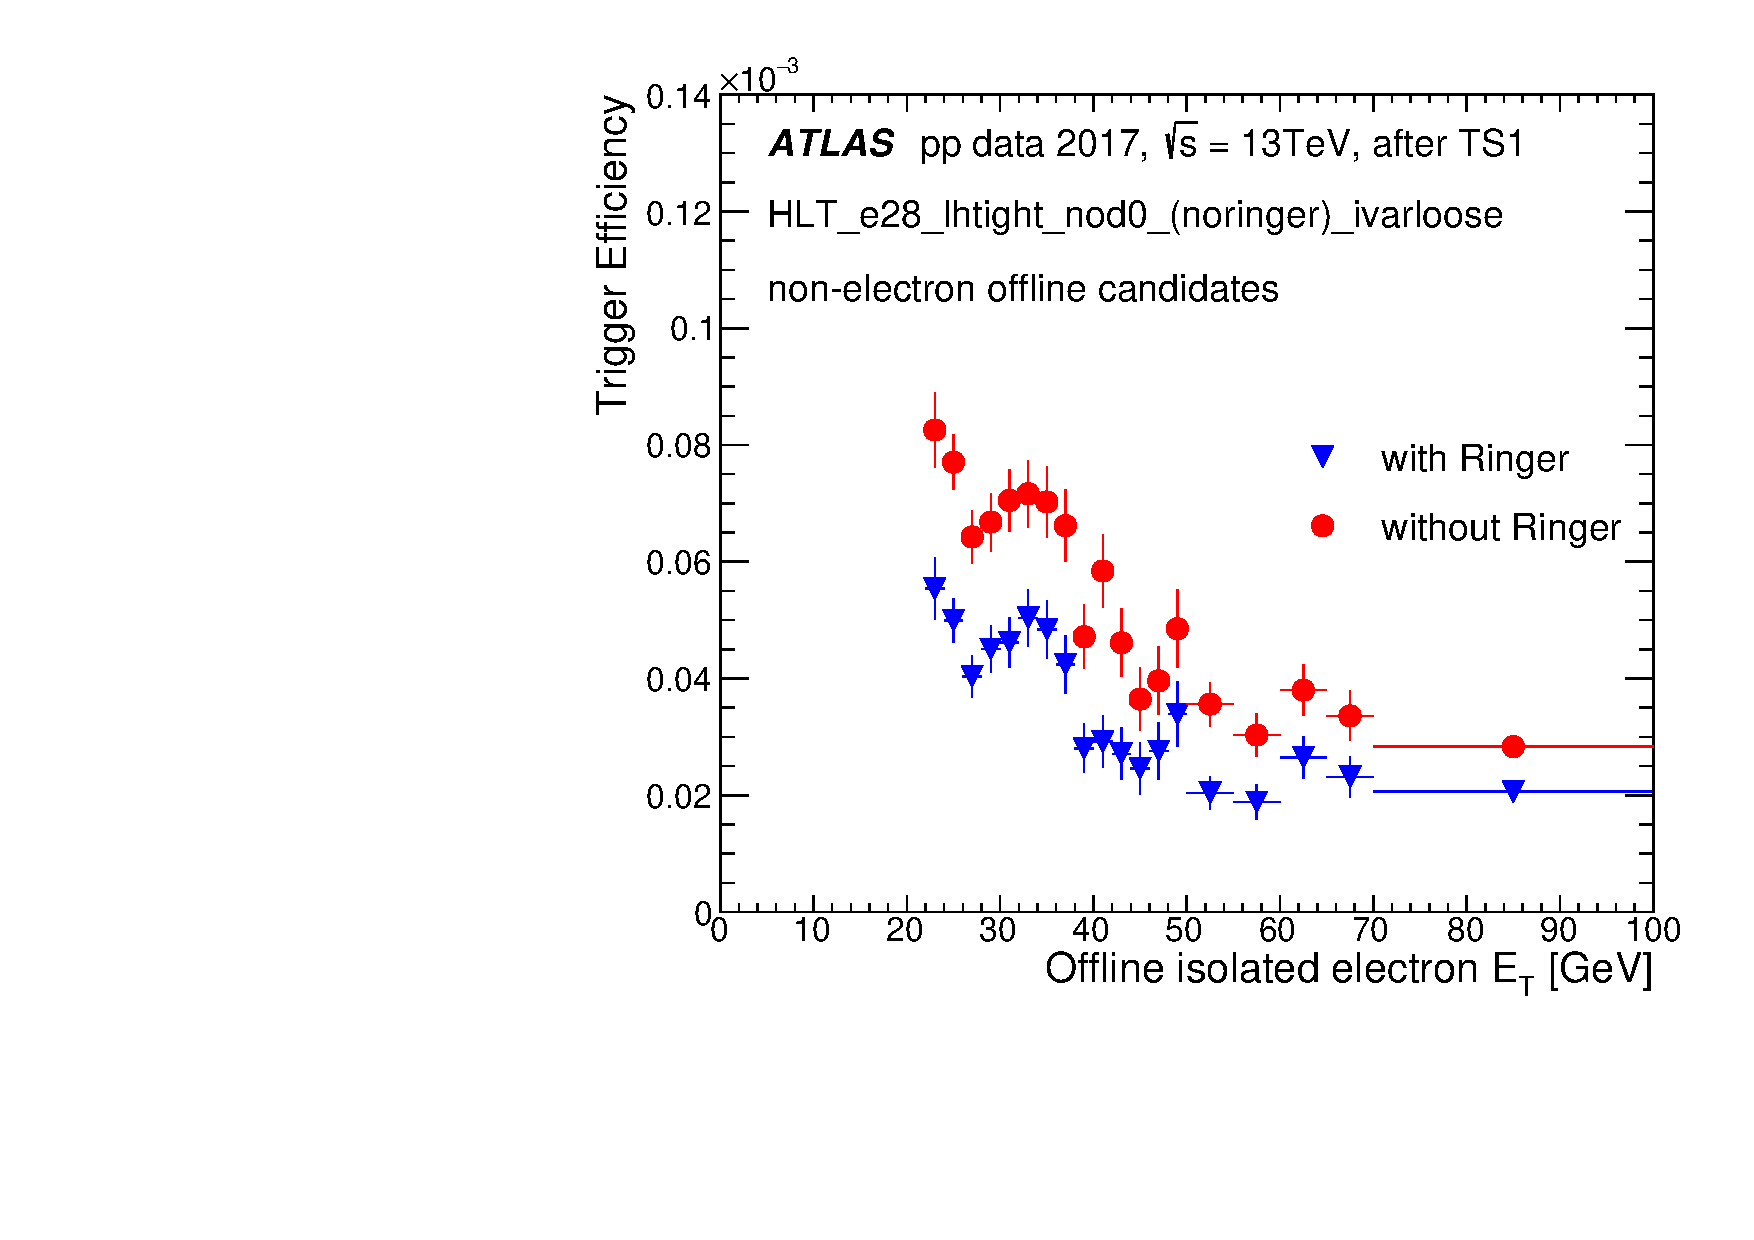
\includegraphics[width=\textwidth]{sections/03_operation/figures/efficiencies/eff_EGAM7_e28_ringer_and_noringer_2017_after_ts1_HLT_et.pdf}
  \caption{}
  \end{subfigure}\\
  %
  \begin{subfigure}[c]{.49\textwidth}
  \centering
  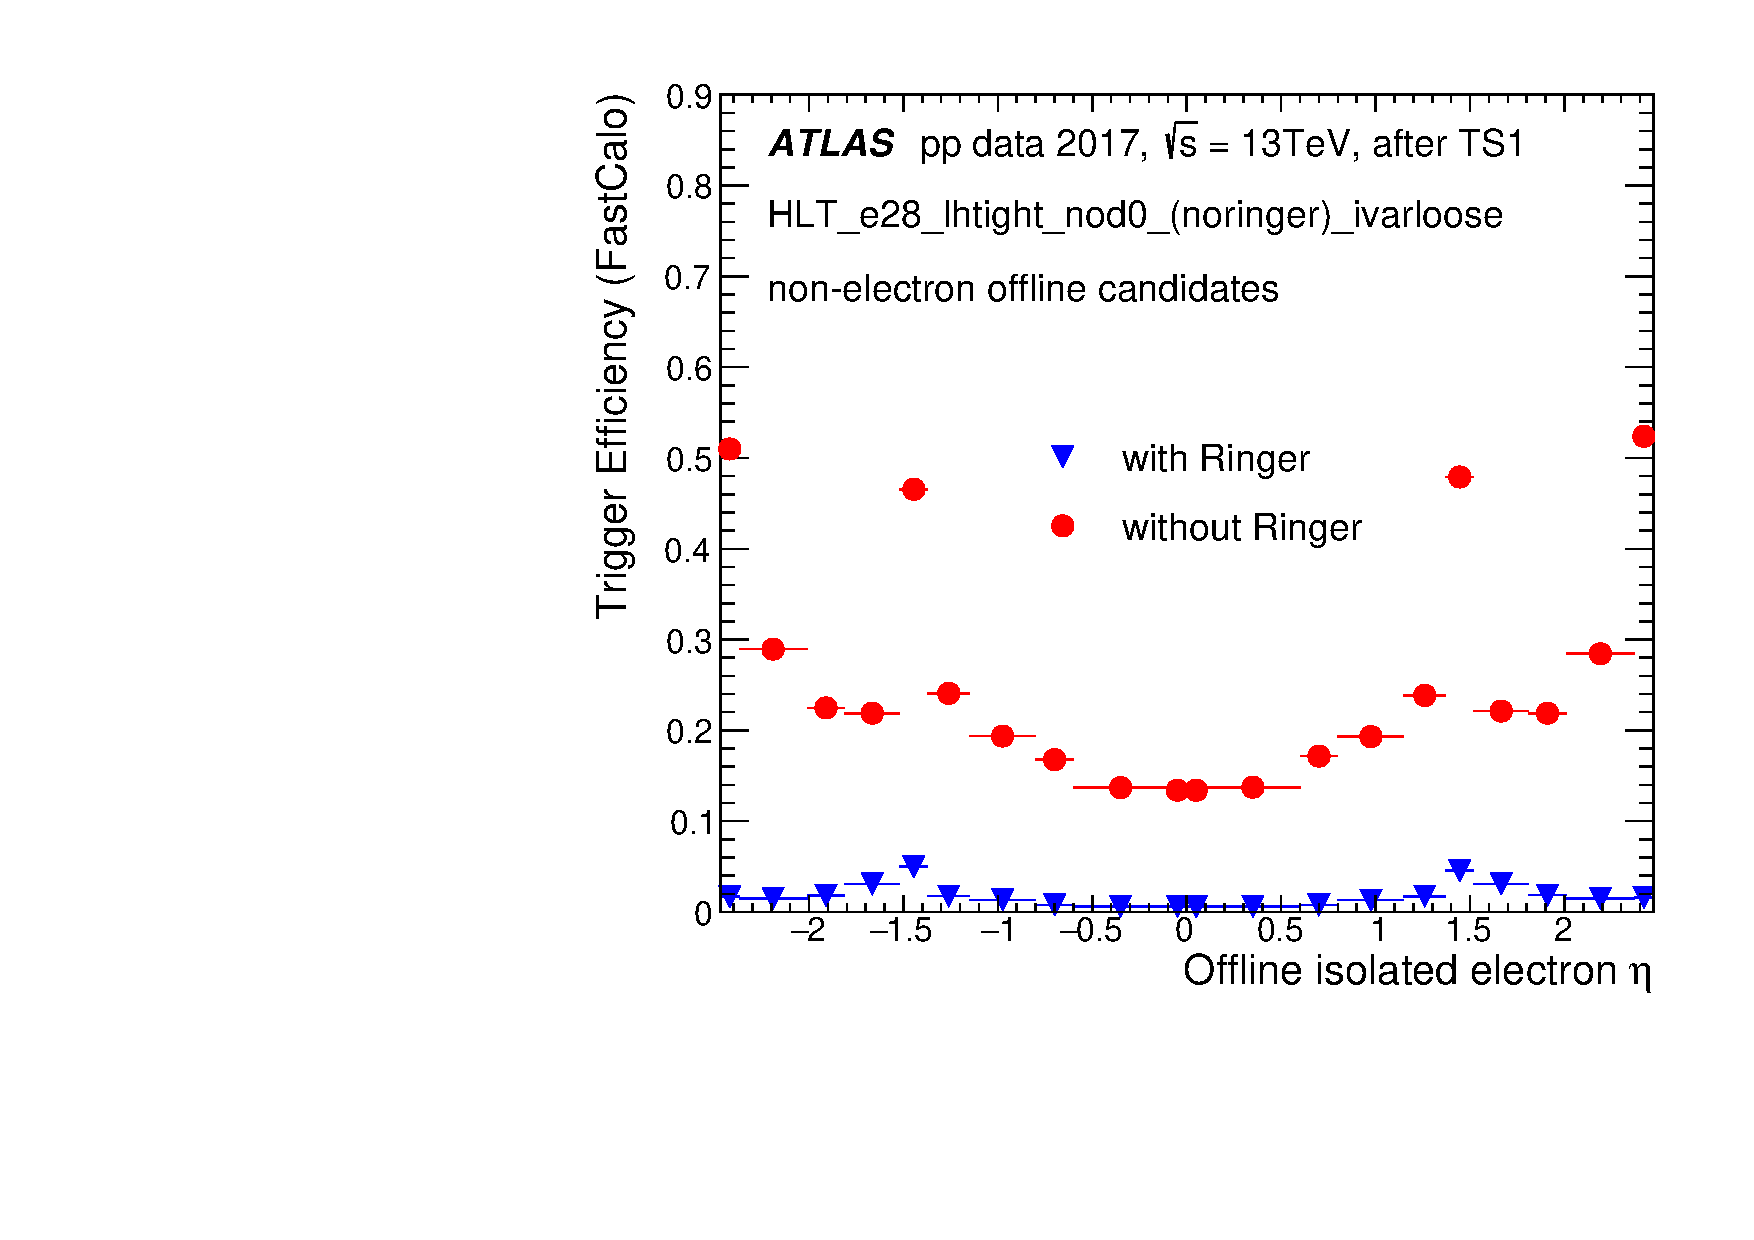
\includegraphics[width=\textwidth]{sections/03_operation/figures/efficiencies/eff_EGAM7_e28_ringer_and_noringer_2017_after_ts1_L2Calo_eta.pdf}
  \caption{}
  \end{subfigure}
  %
  \begin{subfigure}[c]{.49\textwidth}
  \centering
  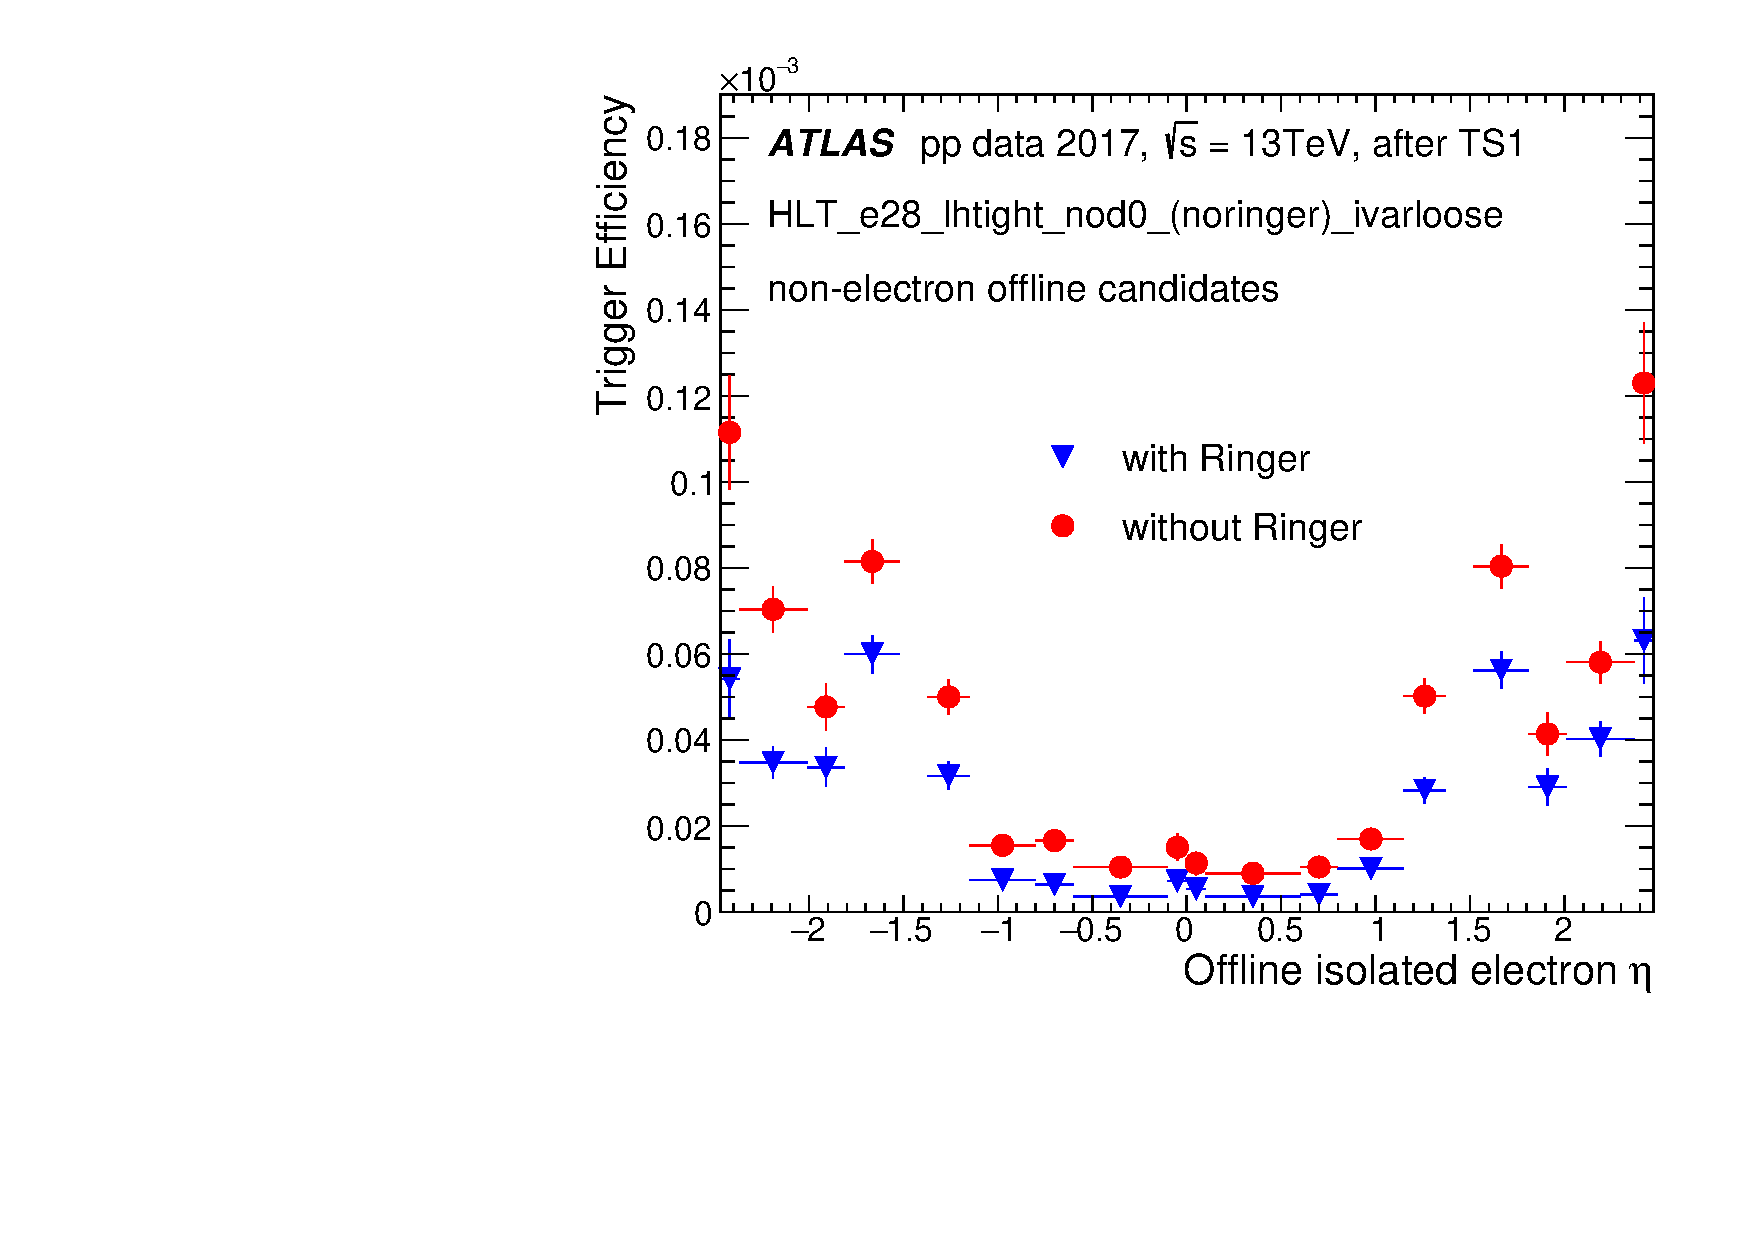
\includegraphics[width=\textwidth]{sections/03_operation/figures/efficiencies/eff_EGAM7_e28_ringer_and_noringer_2017_after_ts1_HLT_eta.pdf}
  \caption{}
  \end{subfigure}\\

  \caption{Efficiency of selecting background at \DIFaddbeginFL \DIFaddFL{the }\DIFaddendFL FastCalo (\DIFdelbeginFL \DIFdelFL{Left}\DIFdelendFL \DIFaddbeginFL \DIFaddFL{left}\DIFaddendFL ) and \DIFdelbeginFL \DIFdelFL{at }\DIFdelendFL HLT (\DIFdelbeginFL \DIFdelFL{Right}\DIFdelendFL \DIFaddbeginFL \DIFaddFL{right}\DIFaddendFL ) \DIFaddbeginFL \DIFaddFL{steps }\DIFaddendFL as a function of \DIFdelbeginFL \DIFdelFL{$E_T$ }\DIFdelendFL \DIFaddbeginFL \ET \DIFaddendFL (\DIFdelbeginFL \DIFdelFL{Top}\DIFdelendFL \DIFaddbeginFL \DIFaddFL{top}\DIFaddendFL ) and $\eta$ (\DIFdelbeginFL \DIFdelFL{Bottom}\DIFdelendFL \DIFaddbeginFL \DIFaddFL{bottom}\DIFaddendFL ) \DIFdelbeginFL \DIFdelFL{for }\DIFdelendFL \DIFaddbeginFL \DIFaddFL{with }\DIFaddendFL a \DIFdelbeginFL \DIFdelFL{single electron isolated }\DIFdelendFL \DIFaddbeginFL \DIFaddFL{single-isolated-electron }\DIFaddendFL trigger requiring $\et > \SI{28}{\GeV}$ and \DIFdelbeginFL \DIFdelFL{tight }\DIFdelendFL \DIFaddbeginFL \enquote{tight} \DIFaddendFL selection, with and without the \rnn{} algorithm, employing 2017 collision data collected after the \rnn algorithm deployment.\DIFdelbeginFL %DIFDELCMD < 

%DIFDELCMD <   
%DIFDELCMD <   %%%
\DIFdelendFL }
  %DIF < 
  \label{fig:2017_fake_triggers_after_ts1}
\DIFdelbeginFL %DIFDELCMD < 

%DIFDELCMD < %%%
\DIFdelendFL \end{figure}

\begin{comment}
    
\begin{figure}[h!tb]
  \begin{subfigure}[c]{.49\textwidth}
  \centering
  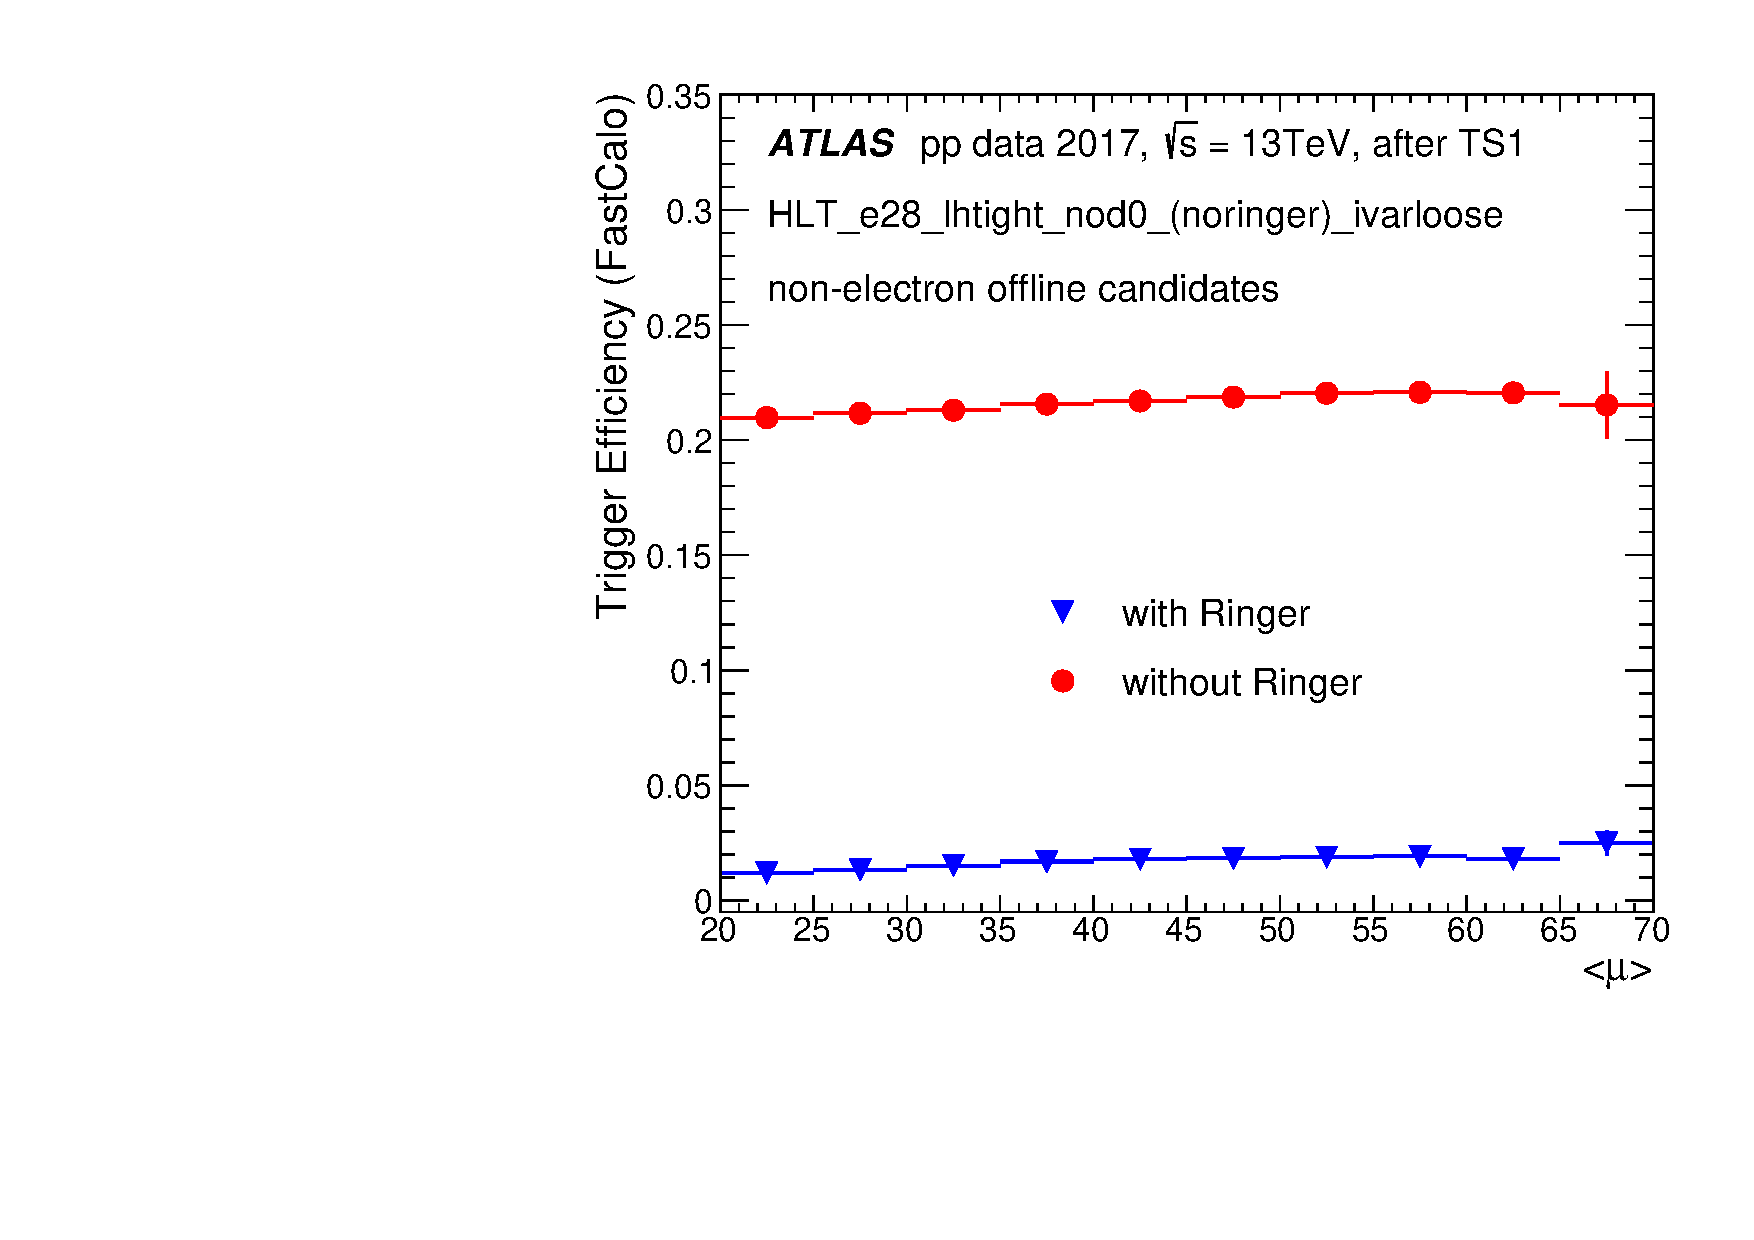
\includegraphics[width=\textwidth]{sections/03_operation/figures/efficiencies/eff_EGAM7_e28_ringer_and_noringer_2017_after_ts1_L2Calo_mu.pdf}
  \caption{}
  \end{subfigure}
  %
  \begin{subfigure}[c]{.49\textwidth}
  \centering
  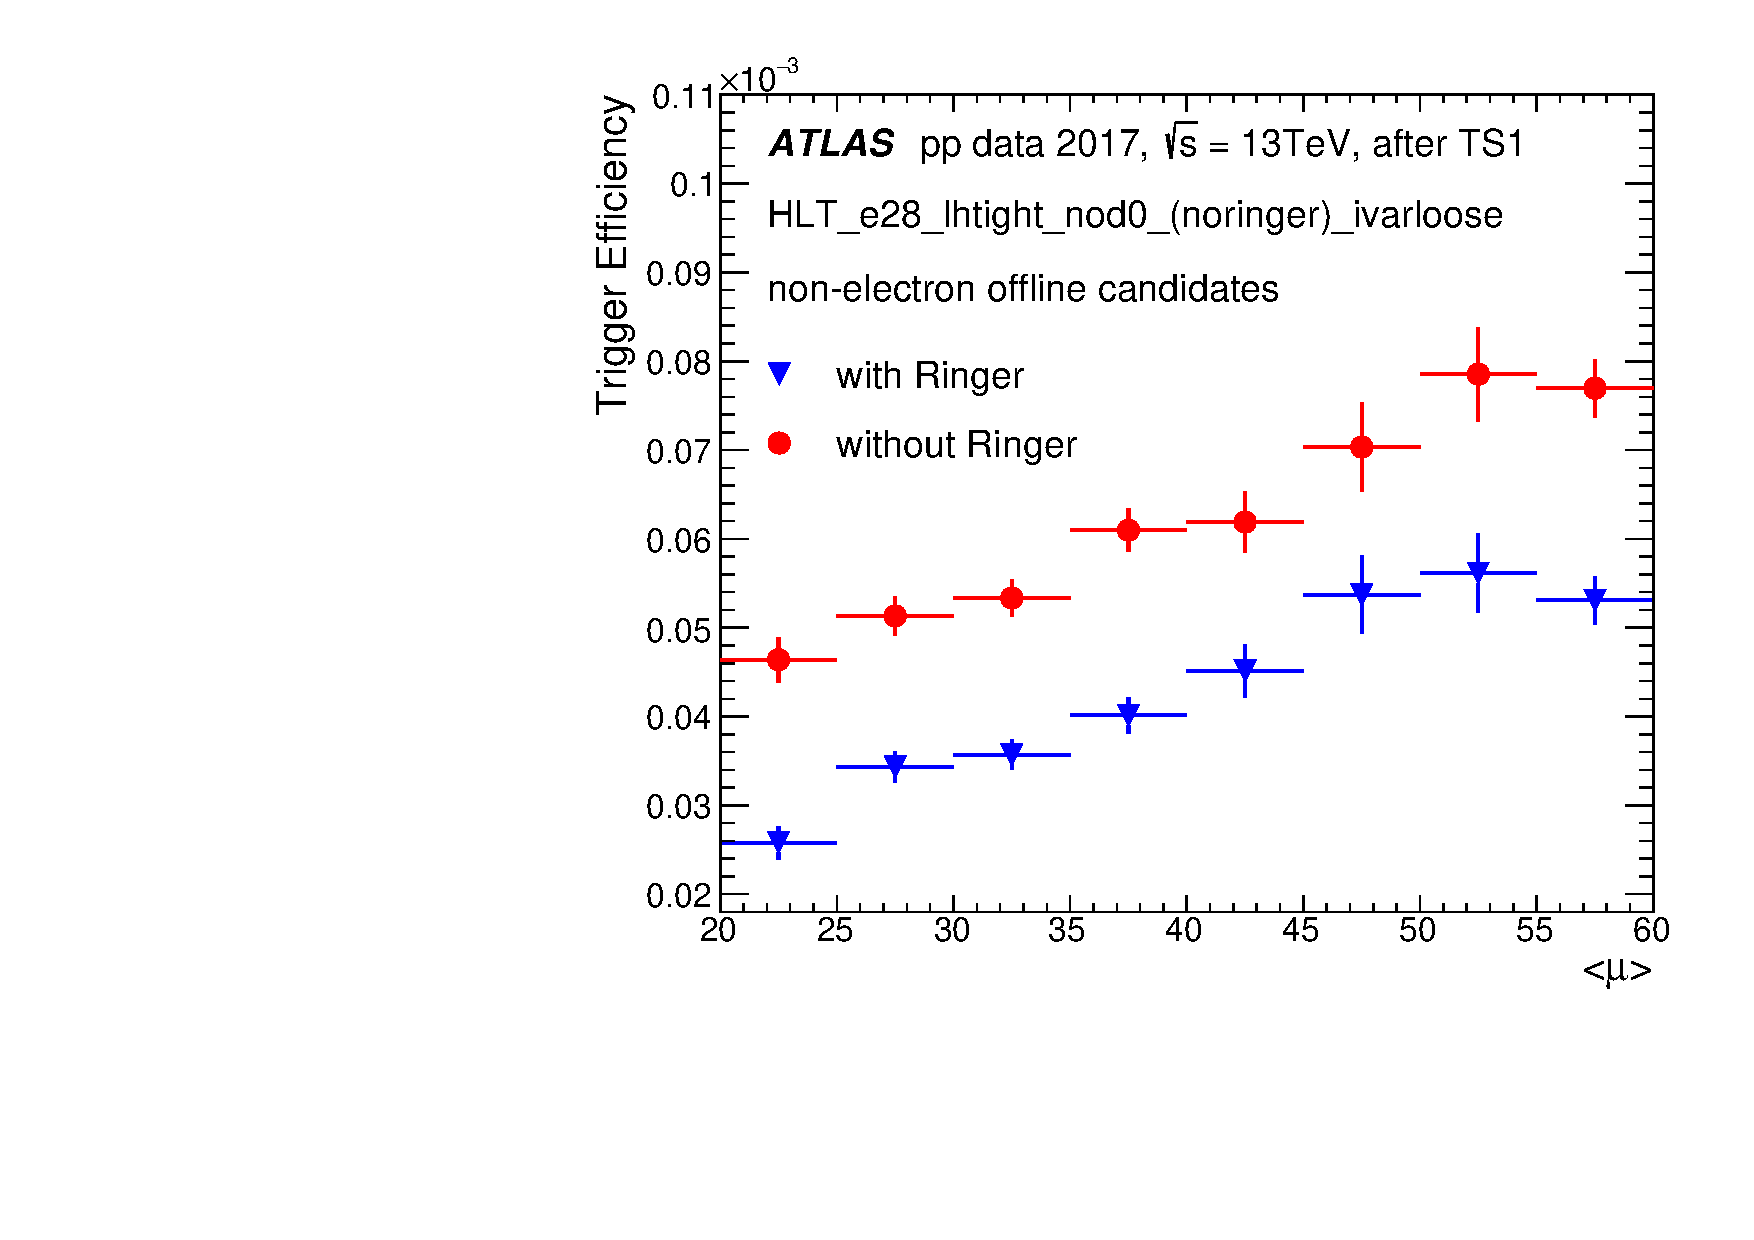
\includegraphics[width=\textwidth]{sections/03_operation/figures/efficiencies/eff_EGAM7_e28_ringer_and_noringer_2017_after_ts1_HLT_mu.pdf}
  \caption{}
  \end{subfigure}

  \caption{ The single electron isolated trigger requiring $\et > \SI{28}{\GeV}$ and \tight selection with and without the \rnn{} algorithm employing 2017 collision data collected after the \rnn algorithm deployment. Left: \fastcalo fake electron efficiency as a function of \avgmu (a). Right: HLT fake electron efficiency as a function of \avgmu (b).}%
  \label{fig:2017_fake_triggers}
\end{figure}
\end{comment}

\subsection{2018 \DIFdelbegin \DIFdel{Operation}\DIFdelend \DIFaddbegin \DIFadd{operation}\DIFaddend }\label{ssec:2018_ringer_operation}

\DIFdelbegin \DIFdel{In }\DIFdelend \DIFaddbegin \DIFadd{For }\DIFaddend 2018 \DIFaddbegin \DIFadd{operation}\DIFaddend , the \rnn{} \DIFdelbegin \DIFdel{operated with a new tune based on }\DIFdelend \DIFaddbegin \DIFadd{was retuned using }\DIFaddend collision data. 
%It was also the case for the final HLT
%selection\footnote{One exception was the \medium{} selection, where the HLT likelihood selection operated in 2018 with the same 2017 tune.}. 
\DIFdelbegin \DIFdel{For the lowest-transverse energy-threshold unprescaled trigger , an efficiency improvement of at least one percentage point in central value is observed when comparing both periods, resulting from a }\DIFdelend \DIFaddbegin \DIFadd{The efficiency of the lowest-transverse-energy-threshold unprescaled trigger increased by at least 1\%, due to }\DIFaddend better operation in all selection steps, \DIFdelbegin \DIFdel{but, in particular, this is due to improvements from }\DIFdelend \DIFaddbegin \DIFadd{and particularly from improvements in }\DIFaddend the likelihood tunes\DIFdelbegin \DIFdel{in the period}\DIFdelend .

\DIFdelbegin \DIFdel{Despite }\DIFdelend \DIFaddbegin \DIFadd{As well as }\DIFaddend maintaining high electron efficiency, \DIFaddbegin \DIFadd{some unprescaled triggers were observed to achieve }\DIFaddend a small reduction in \DIFdelbegin \DIFdel{fake acceptance was observed }\DIFdelend \DIFaddbegin \DIFadd{fake-electron acceptance }\DIFaddend at the  \fastcalo{} step \DIFdelbegin \DIFdel{for some unprescaled triggers }\DIFdelend in comparison with 2017 \DIFaddbegin \DIFadd{operation }\DIFaddend after TS1. For the \DIFdelbegin \DIFdel{lowest-transverse energy-threshold the fake }\DIFdelend \DIFaddbegin \DIFadd{lowest-}\ET\DIFadd{-threshold trigger, the fake-electron }\DIFaddend acceptance was reduced by a factor \DIFdelbegin \DIFdel{by }\DIFdelend \DIFaddbegin \DIFadd{of }\DIFaddend 1.19\DIFdelbegin \DIFdel{. On the other hand, for the highest-transverse energy }\DIFdelend \DIFaddbegin \DIFadd{, while for the highest-}\ET\DIFadd{-threshold }\DIFaddend trigger, a reduction factor \DIFdelbegin \DIFdel{by }\DIFdelend \DIFaddbegin \DIFadd{of }\DIFaddend 1.69 was achieved.


\subsection{Impact on CPU \DIFdelbegin \DIFdel{Demands}\DIFdelend \DIFaddbegin \DIFadd{demands}\DIFaddend } \label{ssec:cpu_reduction}

As observed in the efficiency measurements during \DIFdelbegin \DIFdel{2017-2018 data taking}\DIFdelend \DIFaddbegin \DIFadd{2017--2018 data-taking}\DIFaddend , the \rnn{} allowed \DIFdelbegin \DIFdel{for a }\DIFdelend more effective \fastcalo{} operation \DIFdelbegin \DIFdel{in triggers with electrons above }%DIFDELCMD < \SI{15}{\GeV}  %%%
\DIFdel{with respect to }\DIFdelend \DIFaddbegin \DIFadd{than with }\DIFaddend the previous cut-based approach \DIFaddbegin \DIFadd{for triggers requiring electron }\ET \DIFadd{above }\SI{15}{\GeV}\DIFaddend . 

The overhead required to compute the NN decision \DIFaddbegin \DIFadd{was evaluated }\DIFaddend by running a \DIFdelbegin \DIFdel{single electron }\DIFdelend \DIFaddbegin \DIFadd{single-electron }\DIFaddend trigger with and without the \rnn algorithm, in two individual non-concurrent executions using the same dedicated node\DIFaddbegin \DIFadd{. }\DIFaddend %\footnote{It was used a techlab node Xeon Phi 7120 (1.7 GHz, 32 threads) with 256 Gb@1333 of memory and a SL6 OS.}
\DIFdelbegin \DIFdel{, was evaluated. }\DIFdelend It should be mentioned that, in order to reduce implementation \DIFdelbegin \DIFdel{efforts}\DIFdelend \DIFaddbegin \DIFadd{effort}\DIFaddend , electron triggers \DIFdelbegin \DIFdel{executing the }\DIFdelend \DIFaddbegin \DIFadd{using }\DIFaddend \rnn{} information compute their \DIFdelbegin \DIFdel{information }\DIFdelend \DIFaddbegin \DIFadd{decision }\DIFaddend after the cut-based reconstruction, \DIFdelbegin \DIFdel{whose }\DIFdelend \DIFaddbegin \DIFadd{for which a trigger }\DIFaddend decision is not computed. As a result of this, the \rnn{} electron triggers always demand additional \fastcalo processing time.

Figures~\ref{fig:fastcalo_fex_time} and~\ref{fig:fastcalo_hypo_time} show \DIFdelbegin \DIFdel{the comparison }\DIFdelend \DIFaddbegin \DIFadd{comparisons }\DIFaddend of the total processing time per call for the feature extraction and \DIFdelbegin \DIFdel{hypothesis }\DIFdelend \DIFaddbegin \DIFadd{hypothesis-testing }\DIFaddend algorithms in the \fastcalo \DIFdelbegin \DIFdel{respectively (See }\DIFdelend \DIFaddbegin \DIFadd{step respectively (see }\DIFaddend the related \fastcalo \DIFdelbegin \DIFdel{gray }\DIFdelend blocks in Figure~\ref{fig:electron_chain}). The processing time per call does not include the online data preparation time. The measurements \DIFdelbegin \DIFdel{were evaluated from }\DIFdelend \DIFaddbegin \DIFadd{are based on }\DIFaddend a very loose \DIFdelbegin \DIFdel{selection electron trigger}\DIFdelend \DIFaddbegin \DIFadd{electron trigger, }\DIFaddend with individual executions in the same dedicated computer node.


The measurement employed events from the enhanced bias (EB)
stream~\cite{eb_description} typically extracted from \DIFdelbegin \DIFdel{one hour acquisition }\DIFdelend \DIFaddbegin \DIFadd{a one-hour acquisition period }\DIFaddend with
a specific trigger menu based only on \DIFdelbegin \DIFdel{first level selection and aiming at
}\DIFdelend \DIFaddbegin \DIFadd{first-level selections and a goal of
}\DIFaddend collecting about one\DIFaddbegin \DIFadd{~}\DIFaddend million background events more likely to be accepted by the
\hlt{}. This \DIFdelbegin \DIFdel{behavior is obtained by applying an }\DIFdelend \DIFaddbegin \DIFadd{is achieved by applying }\DIFaddend increased weighting in \DIFaddbegin \DIFadd{the }\DIFaddend high-\pt{} region,
and at \DIFdelbegin \DIFdel{a }\DIFdelend \DIFaddbegin \DIFadd{an }\DIFaddend output trigger rate of \SI{300}{\hertz}~\cite{eb_specifications} for one\DIFaddbegin \DIFadd{~}\DIFaddend hour. 
Hence, the measurements are performed under pile-up conditions\DIFdelbegin \DIFdel{with the execution of the
reconstructed observable algorithm }\DIFdelend \DIFaddbegin \DIFadd{, with the 
reconstruction algorithm executing }\DIFaddend for multiple RoIs in the same bunch-crossing event.


\begin{figure}[h!tb]
	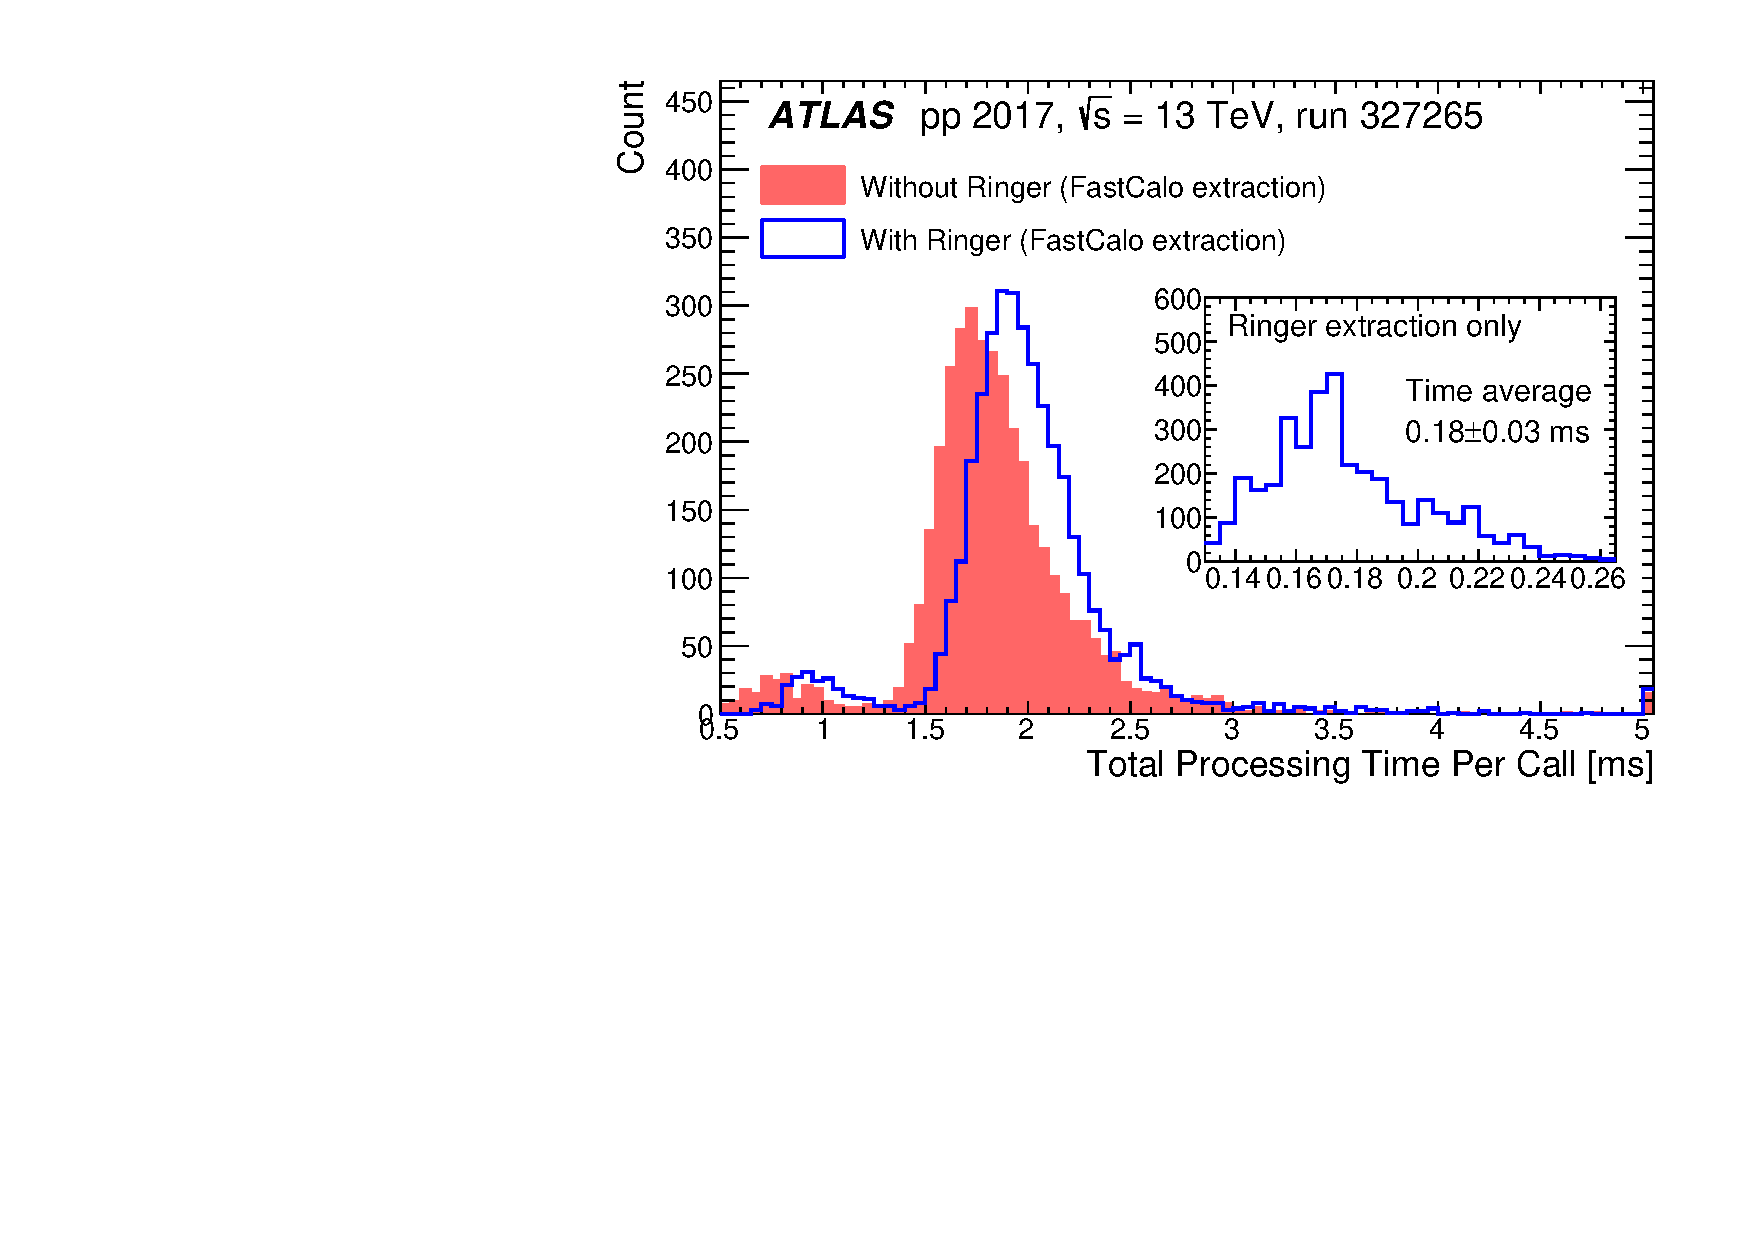
\includegraphics[width=.7\textwidth]{sections/03_operation/figures/EgammaFex_TotalTime}
	\centering
	\caption{\label{fig:fastcalo_fex_time}
		Total processing time per call for the feature extraction algorithms in the \fastcalo step of electron \DIFdelbeginFL \DIFdelFL{offline rerunning }\DIFdelendFL triggers \DIFaddbeginFL \DIFaddFL{rerunning offline, }\DIFaddendFL with (blue) and without (red) \DIFaddbeginFL \DIFaddFL{the }\DIFaddendFL \rnn{}\DIFdelbeginFL \DIFdelFL{using }\DIFdelendFL \DIFaddbeginFL \DIFaddFL{, on }\DIFaddendFL EB events (\DIFdelbeginFL \DIFdelFL{$\avgmu=45$ }\DIFdelendFL peak \DIFaddbeginFL \DIFaddFL{$\avgmu=45$}\DIFaddendFL ). \DIFdelbeginFL \DIFdelFL{Detail }\DIFdelendFL \DIFaddbeginFL \DIFaddFL{The inset }\DIFaddendFL on the right shows the \DIFdelbeginFL \DIFdelFL{individual }\DIFdelendFL processing time per call \DIFdelbeginFL \DIFdelFL{of }\DIFdelendFL \DIFaddbeginFL \DIFaddFL{for only }\DIFaddendFL the ring variable extraction.  
	}
\end{figure}

\begin{figure}[h!tb]
	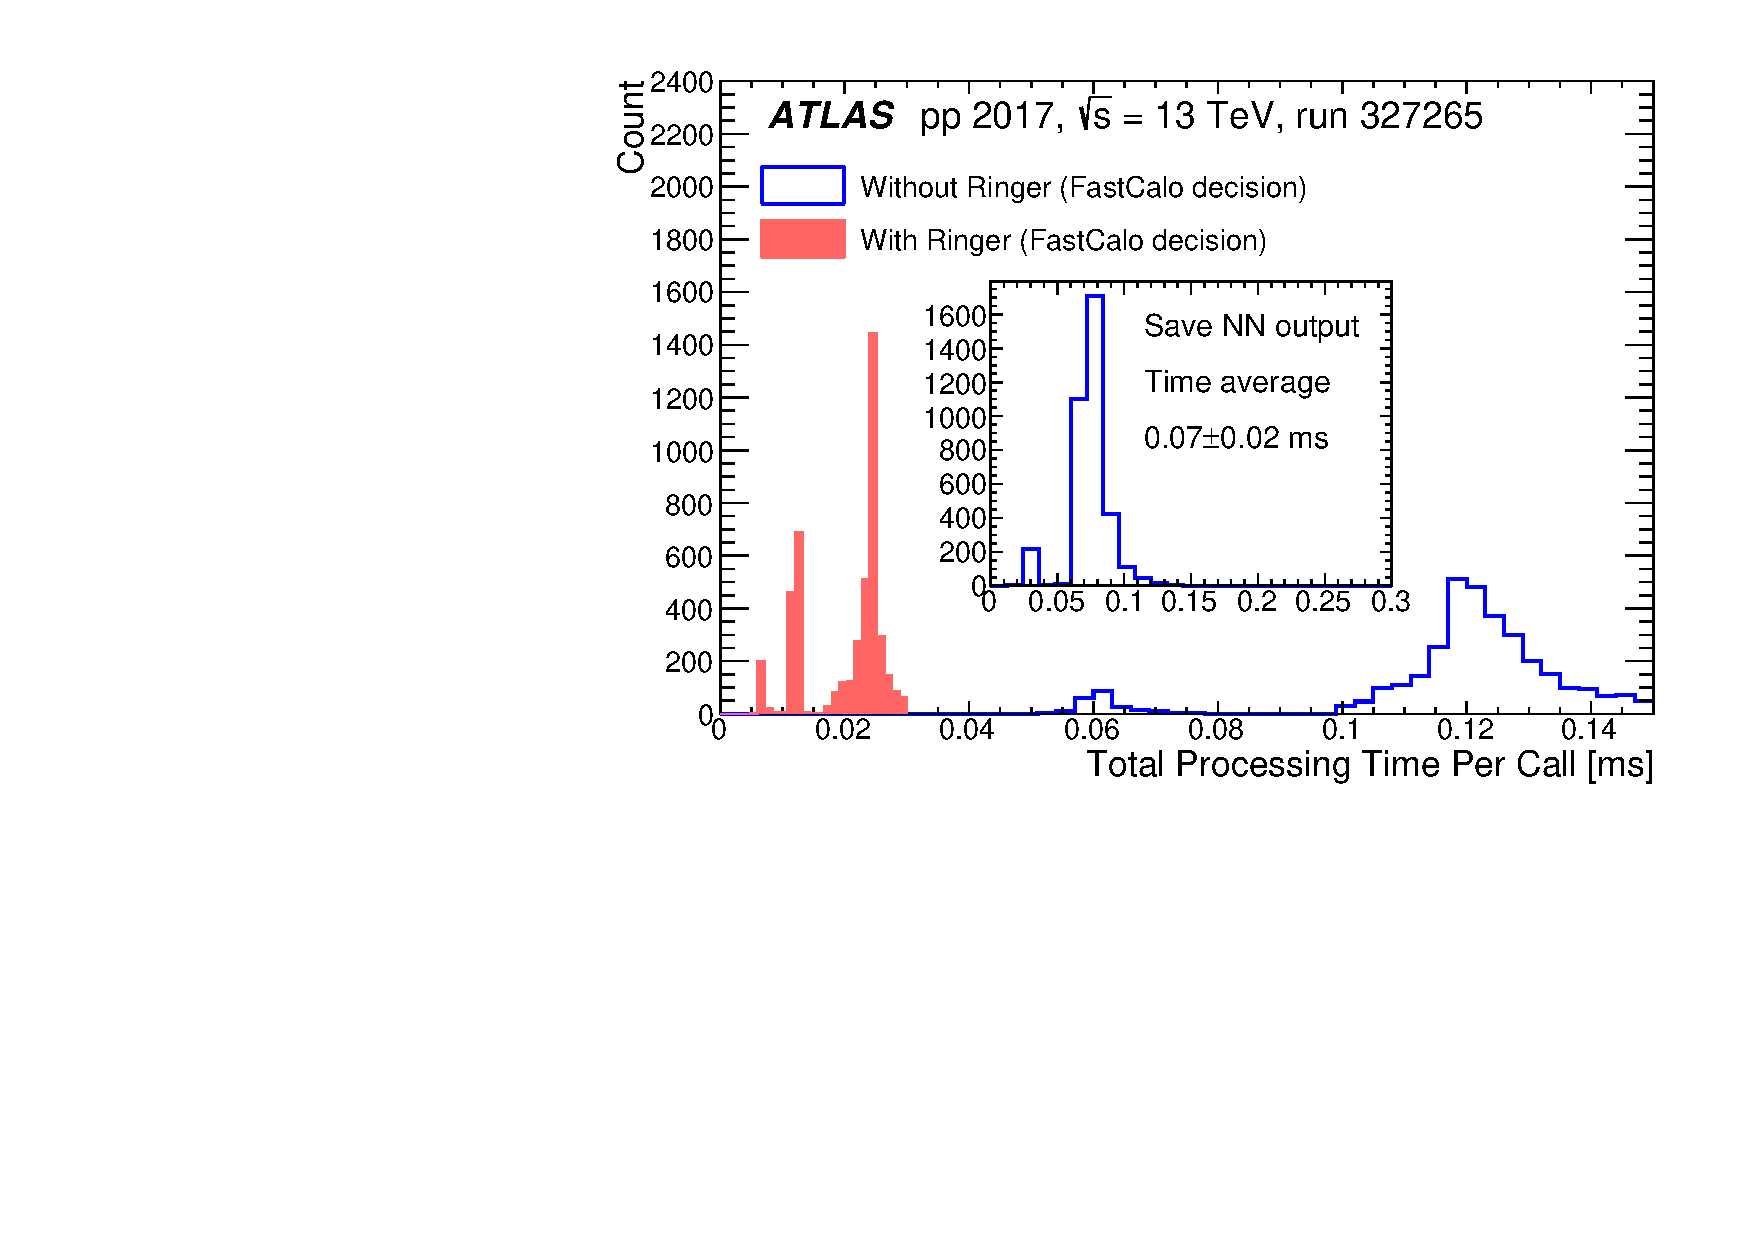
\includegraphics[width=.7\textwidth]{sections/03_operation/figures/EgammaHypo_TotalTime.pdf}
	\centering
	\caption{\label{fig:fastcalo_hypo_time}
		Total processing time per call for the \DIFdelbeginFL \DIFdelFL{hypothesis testing }\DIFdelendFL \DIFaddbeginFL \DIFaddFL{hypothesis-testing }\DIFaddendFL algorithms
		in the \fastcalo step of electron \DIFdelbeginFL \DIFdelFL{offline rerunning }\DIFdelendFL triggers \DIFaddbeginFL \DIFaddFL{rerunning offline, }\DIFaddendFL with (blue) and without (red) \DIFaddbeginFL \DIFaddFL{the }\DIFaddendFL \rnn{}\DIFdelbeginFL \DIFdelFL{using }\DIFdelendFL \DIFaddbeginFL \DIFaddFL{, on }\DIFaddendFL EB events (\DIFdelbeginFL \DIFdelFL{$\langle \mu \rangle = 45$ }\DIFdelendFL peak \DIFaddbeginFL \DIFaddFL{$\langle \mu \rangle = 45$}\DIFaddendFL ). 
		The \DIFdelbeginFL \DIFdelFL{center }\DIFdelendFL \DIFaddbeginFL \DIFaddFL{centre }\DIFaddendFL histogram represents the \DIFdelbeginFL \DIFdelFL{individual }\DIFdelendFL processing time per call to store the \DIFaddbeginFL \DIFaddFL{whole }\DIFaddendFL \rnn{} output in persistent file format.}
\end{figure}

A multi-modal structure can be observed in the feature extraction distributions of both trigger configurations\DIFdelbegin \DIFdel{, which is associated to }\DIFdelend \DIFaddbegin \DIFadd{; it is associated with }\DIFaddend the algorithm for retrieving the EM2 \DIFdelbegin \DIFdel{cells }\DIFdelend \DIFaddbegin \DIFadd{cell energies }\DIFaddend and building related \DIFdelbegin \DIFdel{shower shape
variables}\footnote{\DIFdel{The three peak structure comes from the raw data conversion. Particularly, these are amongst the most-demanding contributions to the }%DIFDELCMD < \fastcalo %%%
\DIFdel{total CPU time.}}%DIFAUXCMD
\addtocounter{footnote}{-1}%DIFAUXCMD
\DIFdel{.}\DIFdelend \DIFaddbegin \DIFadd{shower-shape
variables.}\footnote{\DIFadd{The three-peak structure comes from the raw data conversion. This makes one of the largest demands contributing to }\fastcalo \DIFadd{total CPU time.}} \DIFaddend The computation of the ring variables, \DIFaddbegin \DIFadd{which is }\DIFaddend the only difference between the triggers in the \fastcalo feature extraction, requires an additional average processing time of \DIFdelbegin %DIFDELCMD < \SI{0.18 \pm 0.03}{\ms/\text{event}}%%%
\DIFdelend \DIFaddbegin \DIFadd{$0.18 \pm 0.03$~ms/event}\DIFaddend . 


A \DIFdelbegin \DIFdel{less relevant }\DIFdelend \DIFaddbegin \DIFadd{smaller }\DIFaddend contribution comes from hypothesis testing, in which the ring variables are normalized, the discriminating \DIFaddbegin \DIFadd{variable's }\DIFaddend value is computed, compared \DIFdelbegin \DIFdel{to }\DIFdelend \DIFaddbegin \DIFadd{with }\DIFaddend the selection requirement\DIFdelbegin \DIFdel{and stored into the }\DIFdelend \DIFaddbegin \DIFadd{, and stored in }\DIFaddend persistent file format\DIFdelbegin \footnote{\DIFdel{For Run-3 this step has been removed as a way to reduce the CPU time at }%DIFDELCMD < \fastcalo %%%
\DIFdel{step.}}%DIFAUXCMD
\addtocounter{footnote}{-1}%DIFAUXCMD
\DIFdel{.Specifically, }%DIFDELCMD < \rnn{} %%%
\DIFdel{hypothesis testing }\DIFdelend \DIFaddbegin \DIFadd{.}\footnote{\DIFadd{For }\RunThr\DIFadd{, this step has been removed as a way to reduce the CPU time at the }\fastcalo \DIFadd{step.}}  \DIFadd{Specifically, hypothesis testing for the }\rnn{} \DIFaddend is considerably more \DIFdelbegin \DIFdel{demanding, }\DIFdelend \DIFaddbegin \DIFadd{time-demanding (}\DIFaddend up to \SI{0.14}{\ms/\text{event}}, mostly due to \DIFdelbegin \DIFdel{the time 
}\DIFdelend \DIFaddbegin \DIFadd{taking  
$0.07 \pm 0.02$~ms/event }\DIFaddend to store the \DIFdelbegin \DIFdel{neural network output}%DIFDELCMD < \SI{0.07 \pm 0.02}{\ms/\text{event}}%%%
\DIFdel{, 
}\DIFdelend \DIFaddbegin \DIFadd{neural-network output) }\DIFaddend than the cut-based selection (\SI{0.02}{\ms/\text{event}}), \DIFdelbegin \DIFdel{however small with respect to the feature extractionvalues}\DIFdelend \DIFaddbegin \DIFadd{but less time-demanding than  feature extraction}\DIFaddend . Additionally, the time increase \DIFdelbegin \DIFdel{when compared to }\DIFdelend \DIFaddbegin \DIFadd{is negligible in comparison with }\DIFaddend the average processing time of a \DIFdelbegin \DIFdel{single electron }\DIFdelend \DIFaddbegin \DIFadd{single-electron }\DIFaddend trigger across the entire HLT \DIFdelbegin \DIFdel{is still negligible }\DIFdelend ($\approx 500$\DIFdelbegin \DIFdel{ms in Run 2}\DIFdelend \DIFaddbegin \DIFadd{~ms in }\RunTwo\DIFaddend ).

Taking \DIFdelbegin \DIFdel{into account the referred values}\DIFdelend \DIFaddbegin \DIFadd{these values into account}\DIFaddend , the \rnn{} can require \DIFdelbegin \DIFdel{a
relative increase of }\DIFdelend up to \SI{50}{\%} \DIFdelbegin \DIFdel{in the }\DIFdelend \DIFaddbegin \DIFadd{more }\DIFaddend \fastcalo{} CPU time per event
\DIFdelbegin \DIFdel{with respect to }\DIFdelend \DIFaddbegin \DIFadd{than }\DIFaddend the trigger without \DIFaddbegin \DIFadd{the }\DIFaddend \rnn{}\DIFdelbegin \footnote{\DIFdel{It is expected that the result be dependent on the trigger configuration due to presence of pile-up. Reported results are for HLT\_e17\_lhvloose\_nod0 single electron trigger.}}%DIFAUXCMD
\addtocounter{footnote}{-1}%DIFAUXCMD
\DIFdel{.}\DIFdelend \DIFaddbegin \DIFadd{.}\footnote{\DIFadd{The CPU-time increase is expected to depend on the trigger configuration because of the presence of pile-up. The reported results are for the HLT\_e17\_lhvloose\_nod0 single-electron trigger.}} \DIFaddend Nonetheless, the \rnn{} \DIFdelbegin \DIFdel{contributes to }\DIFdelend \DIFaddbegin \DIFadd{provides }\DIFaddend a more discriminating selection, \DIFdelbegin \DIFdel{allowing to reduce CPU demanding }\DIFdelend \DIFaddbegin \DIFadd{which  reduces the number of CPU-demanding }\DIFaddend triggers by reducing the \DIFdelbegin \DIFdel{processing of }\DIFdelend \DIFaddbegin \DIFadd{need to process }\DIFaddend fake electrons in subsequent steps that are more computationally demanding. In this measurement, where about \DIFdelbegin \DIFdel{3,400 }\DIFdelend \DIFaddbegin \DIFadd{3400 }\DIFaddend events from the EB stream were considered, the \rnn{} algorithm provided an overall
\SI{60}{\%} reduction \DIFdelbegin \DIFdel{(}\DIFdelend \DIFaddbegin \DIFadd{in the CPU demands (from }\DIFaddend \SI{30.72}{\milli\second} to \SI{10.36}{\milli\second} \DIFdelbegin \DIFdel{)
in the CPU demands avoiding the computation of fake candidates after }\DIFdelend \DIFaddbegin \DIFadd{per event) by rejecting most fake electron candidates during }\DIFaddend the \fastcalo step. 





 \newpage  % ok
 \newpage 
\section{\rnn{} \DIFdelbegin \DIFdel{Aggreament}\DIFdelend \DIFaddbegin \DIFadd{assessment vs cut-based triggers}\DIFaddend }%
\label{sec:off_ana}

This section \DIFdelbegin \DIFdel{is dedicated to }\DIFdelend \DIFaddbegin \DIFadd{presents }\DIFaddend a more detailed \DIFdelbegin \DIFdel{assessments }\DIFdelend \DIFaddbegin \DIFadd{assessment }\DIFaddend of the \rnn{}\DIFdelbegin \DIFdel{behavior 
}\DIFdelend \DIFaddbegin \DIFadd{'s behaviour 
}\DIFaddend in the period \DIFdelbegin \DIFdel{2017-2018 with respect }\DIFdelend \DIFaddbegin \DIFadd{2017--2018 relative }\DIFaddend to the previous electron trigger\DIFaddbegin \DIFadd{'s }\DIFaddend cut-based strategy.
\DIFdelbegin \DIFdel{Using }\DIFdelend \DIFaddbegin \DIFadd{A }\DIFaddend \Zee{} \tnp{} selection \DIFdelbegin \DIFdel{, the }\DIFdelend \DIFaddbegin \DIFadd{was used to evaluate the level of }\DIFaddend agreement between the two triggers\DIFdelbegin \DIFdel{and
possible biases , caused by the introduction of }\DIFdelend \DIFaddbegin \DIFadd{, 
as well as possible biases due to the variables }\DIFaddend the \rnn{} \DIFdelbegin \DIFdel{using the variables
employed by the likelihood algorithm, were investigated.
Since }\DIFdelend \DIFaddbegin \DIFadd{employs in the likelihood algorithm.
Since both the }\DIFaddend offline and final HLT electron selections are based on such variables, limiting the evaluation 
to \DIFdelbegin \DIFdel{them suffices to understand any }\DIFdelend \DIFaddbegin \DIFadd{those varaibles suffices for understanding the }\DIFaddend possible impact of the \rnn{} algorithm in most analyses.
\DIFdelbegin \DIFdel{Additionally, these variables are interesting since they }\DIFdelend \DIFaddbegin \DIFadd{In addition, it is advantageous to }\DIFaddend compact the input space
\DIFdelbegin \DIFdel{in }\DIFdelend \DIFaddbegin \DIFadd{into }\DIFaddend a set of \DIFdelbegin \DIFdel{few variables with }\DIFdelend \DIFaddbegin \DIFadd{a few such variables that have }\DIFaddend low correlation and \DIFdelbegin \DIFdel{high interpretability power}\DIFdelend \DIFaddbegin \DIFadd{are easy to interpret}\DIFaddend . 
%One should keep in mind that the \rnn{} algorithm had access only to the ring description during Run~2 operation.


Since \DIFdelbegin \DIFdel{the Tag \& Probe events have }\DIFdelend \DIFaddbegin \DIFadd{each }\tnp{} \DIFadd{event has }\DIFaddend one electron, called \DIFdelbegin \DIFdel{as probe electron}\DIFdelend \DIFaddbegin \DIFadd{the probe electron, }\DIFaddend that was not 
used to \DIFdelbegin \DIFdel{decide the selection of }\DIFdelend \DIFaddbegin \DIFadd{select }\DIFaddend that event at \DIFdelbegin \DIFdel{the }\DIFdelend trigger level, two \DIFaddbegin \DIFadd{offline }\DIFaddend analyses were performed to assess the
trigger performance with and without \DIFaddbegin \DIFadd{the }\DIFaddend \rnn{}, \DIFdelbegin \DIFdel{when the selection is applied }\DIFdelend \DIFaddbegin \DIFadd{with the offline selection applied either }\DIFaddend to
the tag electron (Homogeneity Tests\DIFaddbegin }\DIFaddend ) or to the probe \DIFaddbegin \DIFadd{electron }\DIFaddend (Quadrant Analysis\DIFaddbegin }\DIFaddend ). 


The Quadrant Analysis allows \DIFdelbegin \DIFdel{to directly assess possible bias caused by }\DIFdelend \DIFaddbegin \DIFadd{a direct assessment of possible bias due to }\DIFaddend the
introduction of the \rnn{} by comparing the profiles for all possible disjoint
decisions from the two trigger classifiers. \DIFdelbegin \DIFdel{Hence, it }\DIFdelend \DIFaddbegin \DIFadd{It }\DIFaddend is possible for the classifiers
to agree\DIFdelbegin \DIFdel{by both }\DIFdelend \DIFaddbegin \DIFadd{, with both of them }\DIFaddend accepting or rejecting the event. Likewise, they \DIFdelbegin \DIFdel{are able to
}\DIFdelend \DIFaddbegin \DIFadd{can 
}\DIFaddend disagree in two possible \DIFdelbegin \DIFdel{cases where either one decides to accept the event
while the other rejects }\DIFdelend \DIFaddbegin \DIFadd{ways, with one classifier accepting the event
and the other rejecting }\DIFaddend it.

Although it is reasonable to \DIFdelbegin \DIFdel{expect that the shower development of the tag and the probe are independent from each other}\DIFdelend \DIFaddbegin \DIFadd{assume that the tag and probe showers 
develop independently}\DIFaddend , and that the \rnn{} when applied to
the tag selection cannot, in principle, alter the profile of the probes besides
changing the number of \tnp{} pairs\DIFdelbegin \DIFdel{. Such }\DIFdelend \DIFaddbegin \DIFadd{, this assumption should be tested. 
An }\DIFaddend evaluation of any possible systematic effect \DIFdelbegin \DIFdel{caused by the introduction of the }\DIFdelend \DIFaddbegin \DIFadd{due to using the }\DIFaddend \rnn{} 
in \DIFdelbegin \DIFdel{the extraction of the likelihood PDFs, employed }\DIFdelend \DIFaddbegin \DIFadd{obtaining the likelihood probability distribution functions (PDFs), 
used }\DIFaddend for offline and final HLT selection, is performed \DIFdelbegin \DIFdel{by }\DIFdelend \DIFaddbegin \DIFadd{with }\DIFaddend the Homogeneity Tests.



\subsection{Quadrant Analysis}\label{ssec:quadrant}

The Quadrant Analysis was developed to compare the \DIFdelbegin \DIFdel{decision }\DIFdelend \DIFaddbegin \DIFadd{decisions }\DIFaddend of two classifiers. Given signal candidates and two classifiers, these are the possibilities:\DIFaddbegin \DIFadd{\ }\DIFaddend either both accept or reject the candidates\DIFaddbegin \DIFadd{, }\DIFaddend or only one accepts the candidates. The four possible decision quadrants are evaluated from \DIFdelbegin \DIFdel{shower shape }\DIFdelend \DIFaddbegin \DIFadd{shower-shape }\DIFaddend distributions. Furthermore, in this analysis, it \DIFdelbegin \DIFdel{'s }\DIFdelend \DIFaddbegin \DIFadd{is }\DIFaddend also possible to \DIFdelbegin \DIFdel{compare }\DIFdelend \DIFaddbegin \DIFadd{evaluate }\DIFaddend the disagreement between two classifiers. The disagreement between two classifiers $\textbf{A}$ and $\textbf{B}$ can be defined as:

\begin{equation}
    \text{disagreement} = \frac{N_{\textbf{A}}+N_{\textbf{B}}}{N_{\textbf{A}}+N_{\textbf{B}}+N_{\textbf{AB}}+N_{!\textbf{AB}}}
    \label{eq:disagreement}
\end{equation}
where $N_{\textbf{A}}$ ($N_{\textbf{B}}$) is the total \DIFaddbegin \DIFadd{number }\DIFaddend of candidates accepted exclusively by classifier $\textbf{A}$ ($\textbf{B}$) and $N_{\textbf{AB}}$ ($N_{\textbf{!AB}}$) is the total \DIFaddbegin \DIFadd{number }\DIFaddend of candidates accepted (rejected) by both classifiers.

In this approach, only collision data collected \DIFdelbegin \DIFdel{by }\DIFdelend \DIFaddbegin \DIFadd{using }\DIFaddend the primary triggers with an equivalent offline selection are considered\DIFdelbegin \footnote{\DIFdel{I.e., if a }%DIFDELCMD < \tight{} %%%
\DIFdel{trigger leg is being evaluated, it also applied the }%DIFDELCMD < \tight{} %%%
\DIFdel{offline selection to the candidate.}}%DIFAUXCMD
\addtocounter{footnote}{-1}%DIFAUXCMD
\DIFdel{.}\DIFdelend \DIFaddbegin \DIFadd{.}\footnote{\DIFadd{For example, if a }\enquote{tight} \DIFadd{trigger leg is being evaluated, the }\enquote{tight} \DIFadd{offline selection is also applied to the candidate.}}
\DIFaddend Results in Section~\ref{top:quadrant_results} show
trigger selection performance using \DIFdelbegin %DIFDELCMD < \tight{} %%%
\DIFdelend \DIFaddbegin \DIFadd{the }\enquote{tight} \DIFaddend requirement for the duplicated triggers during 2017.

\subsubsection{Results}\label{top:quadrant_results}

The Quadrant Analysis was performed on the \DIFdelbegin \DIFdel{variables ($R_{\eta}$, $R_{\phi}$, $E_{ratio}$ and $R_{had}$}\DIFdelend \DIFaddbegin \DIFadd{four variables (}\reta{}\DIFadd{, }\rphi{}\DIFadd{, }\eratio{} \DIFadd{and }\rhad{}\DIFaddend ) used in the likelihood~\cite{PERF-2017-01} selection \DIFdelbegin \DIFdel{and }\DIFdelend \DIFaddbegin \DIFadd{that }\DIFaddend have the best discrimination power between electrons and jets. 

As shown in Figure~\DIFdelbegin \DIFdel{\ref{fig:quadrant_calo_variables_30GeV_eta}}\DIFdelend \DIFaddbegin \DIFadd{\ref{fig:quadrant_calo_variables_30GeV}}\DIFaddend , the disagreement is small and \DIFdelbegin \DIFdel{bounded for most cases at }\DIFdelend \DIFaddbegin \DIFadd{in most cases bounded at about }\DIFaddend the 1\% level for the coverage of \DIFdelbegin \DIFdel{all calorimetry variables. This behavior }\DIFdelend \DIFaddbegin \DIFadd{each variable. Here, only the results for $0.6<|\eta|<0.8$ and $35<\ET<40$~}\GeV \DIFadd{are shown, but this behaviour }\DIFaddend is also observed for \DIFaddbegin \DIFadd{other }\DIFaddend \et{} regions\DIFaddbegin \DIFadd{, and these results are more representative of those obtained in other regions of the $\eteta$ phase space}\DIFaddend . 
One should note that the working points of \DIFdelbegin \DIFdel{both }\DIFdelend \DIFaddbegin \DIFadd{the two }\DIFaddend triggers are not exactly the same, although the \rnn{} aims \DIFdelbegin \DIFdel{at keeping }\DIFdelend \DIFaddbegin \DIFadd{to achieve }\DIFaddend the same signal efficiency as the cut-based strategy and was operating as desired.  
%Thus, much of the differences reflect this difficulty. 
In other words, 
%One should note that the integral of the single trigger cases is related to the limitation in the precision of setting the working point of both triggers to be exactly the same. In other words, 
the \DIFdelbegin \DIFdel{difference in height of }\DIFdelend \DIFaddbegin \DIFadd{height differences between }\DIFaddend the blue and red profiles in Figure~\DIFdelbegin \DIFdel{\ref{fig:quadrant_calo_variables_30GeV_eta} is }\DIFdelend \DIFaddbegin \DIFadd{\ref{fig:quadrant_calo_variables_30GeV} are }\DIFaddend mainly due to \DIFdelbegin \DIFdel{the small differences in efficiencies }\DIFdelend \DIFaddbegin \DIFadd{small efficiency differences }\DIFaddend between the two triggers.
\DIFdelbegin \DIFdel{Here, only the results for $0.6<|\eta|<0.8$ and $35<E_T\text{[GeV]}<40$ are shown, since these results are more representative of the other results obtained in the rest of the regions of the $\eteta$ phase space.
}\DIFdelend 



%Hence, comparison between profiles is simpler to be performed in the $0.6<\abseta{}<0.8$, which exhibits very similar performance.

\DIFdelbegin \DIFdel{For all variables in this region, both }\DIFdelend \DIFaddbegin \DIFadd{The two }\DIFaddend triggers behave very similarly \DIFdelbegin \DIFdel{(see }\DIFdelend \DIFaddbegin \DIFadd{for all variables in the region shown in }\DIFaddend Figure~\ref{fig:quadrant_calo_variables_30GeV}\DIFdelbegin \DIFdel{)}\DIFdelend , even if some slight shifts \DIFdelbegin \DIFdel{can be observed in few profiles}\DIFdelend \DIFaddbegin \DIFadd{between blue and red profiles can be seen}\DIFaddend . This is the case \DIFdelbegin \DIFdel{of }\DIFdelend \DIFaddbegin \DIFadd{for }\DIFaddend \reta{} and \rphi{}, where the \rnn{} trigger \DIFdelbegin \DIFdel{is consistently collecting }\DIFdelend \DIFaddbegin \DIFadd{consistently selects }\DIFaddend slightly more events in the signal region, i.e.\DIFdelbegin \DIFdel{respectively with slight }\DIFdelend \DIFaddbegin \DIFadd{\ ones with slightly }\DIFaddend tighter showers in $\eta{}$ and $\phi{}$\DIFaddbegin \DIFadd{, respectively, }\DIFaddend in the EM2 \DIFaddbegin \DIFadd{layer}\DIFaddend . The \rnn{} trigger\DIFdelbegin \DIFdel{behavior }\DIFdelend \DIFaddbegin \DIFadd{'s behaviour }\DIFaddend shows an even \DIFdelbegin \DIFdel{lower effect in the }\DIFdelend \DIFaddbegin \DIFadd{smaller effect in }\DIFaddend \rhad{}, where tighter tails are observed, resulting in fewer electrons with 10\% to 30\% \DIFaddbegin \DIFadd{of their }\DIFaddend energy in EM1, 1\% to 2\% in EM3 and more than 4\DIFaddbegin \DIFadd{~}\DIFaddend GeV hadronic leakage. \DIFaddbegin \DIFadd{The }\DIFaddend \eratio{} \DIFdelbegin \DIFdel{also shows a slightly bias towards collecting }\DIFdelend \DIFaddbegin \DIFadd{variable also shows the }\rnn{} \DIFadd{trigger has a slight bias towards selecting }\DIFaddend more events in the signal region\DIFdelbegin \DIFdel{with the }%DIFDELCMD < \rnn{} %%%
\DIFdel{trigger}\DIFdelend . Interestingly, a few events \DIFaddbegin \DIFadd{with $0.5<\eratio{}<0.7$ }\DIFaddend are accepted by the trigger with \DIFaddbegin \DIFadd{the }\DIFaddend \rnn{}, \DIFdelbegin \DIFdel{when $0.5<\eratio{}<0.7$, }\DIFdelend probably due to electrons resulting from premature showers with \DIFdelbegin \DIFdel{barycenter near the edge of }\DIFdelend \DIFaddbegin \DIFadd{a barycentre near the boundary between }\DIFaddend two strips. 
Although similar \DIFdelbegin \DIFdel{behavior is shown for the }\DIFdelend \DIFaddbegin \DIFadd{behaviour is seen in }\DIFaddend other 
regions, the differences vary in strength \DIFdelbegin \DIFdel{in each }\DIFdelend \DIFaddbegin \DIFadd{between }\DIFaddend \abseta{} \DIFdelbegin \DIFdel{region}\DIFdelend \DIFaddbegin \DIFadd{regions}\DIFaddend . 


\begin{figure}[h!]
\centering
\begin{subfigure}[c]{.49\textwidth}
\centering
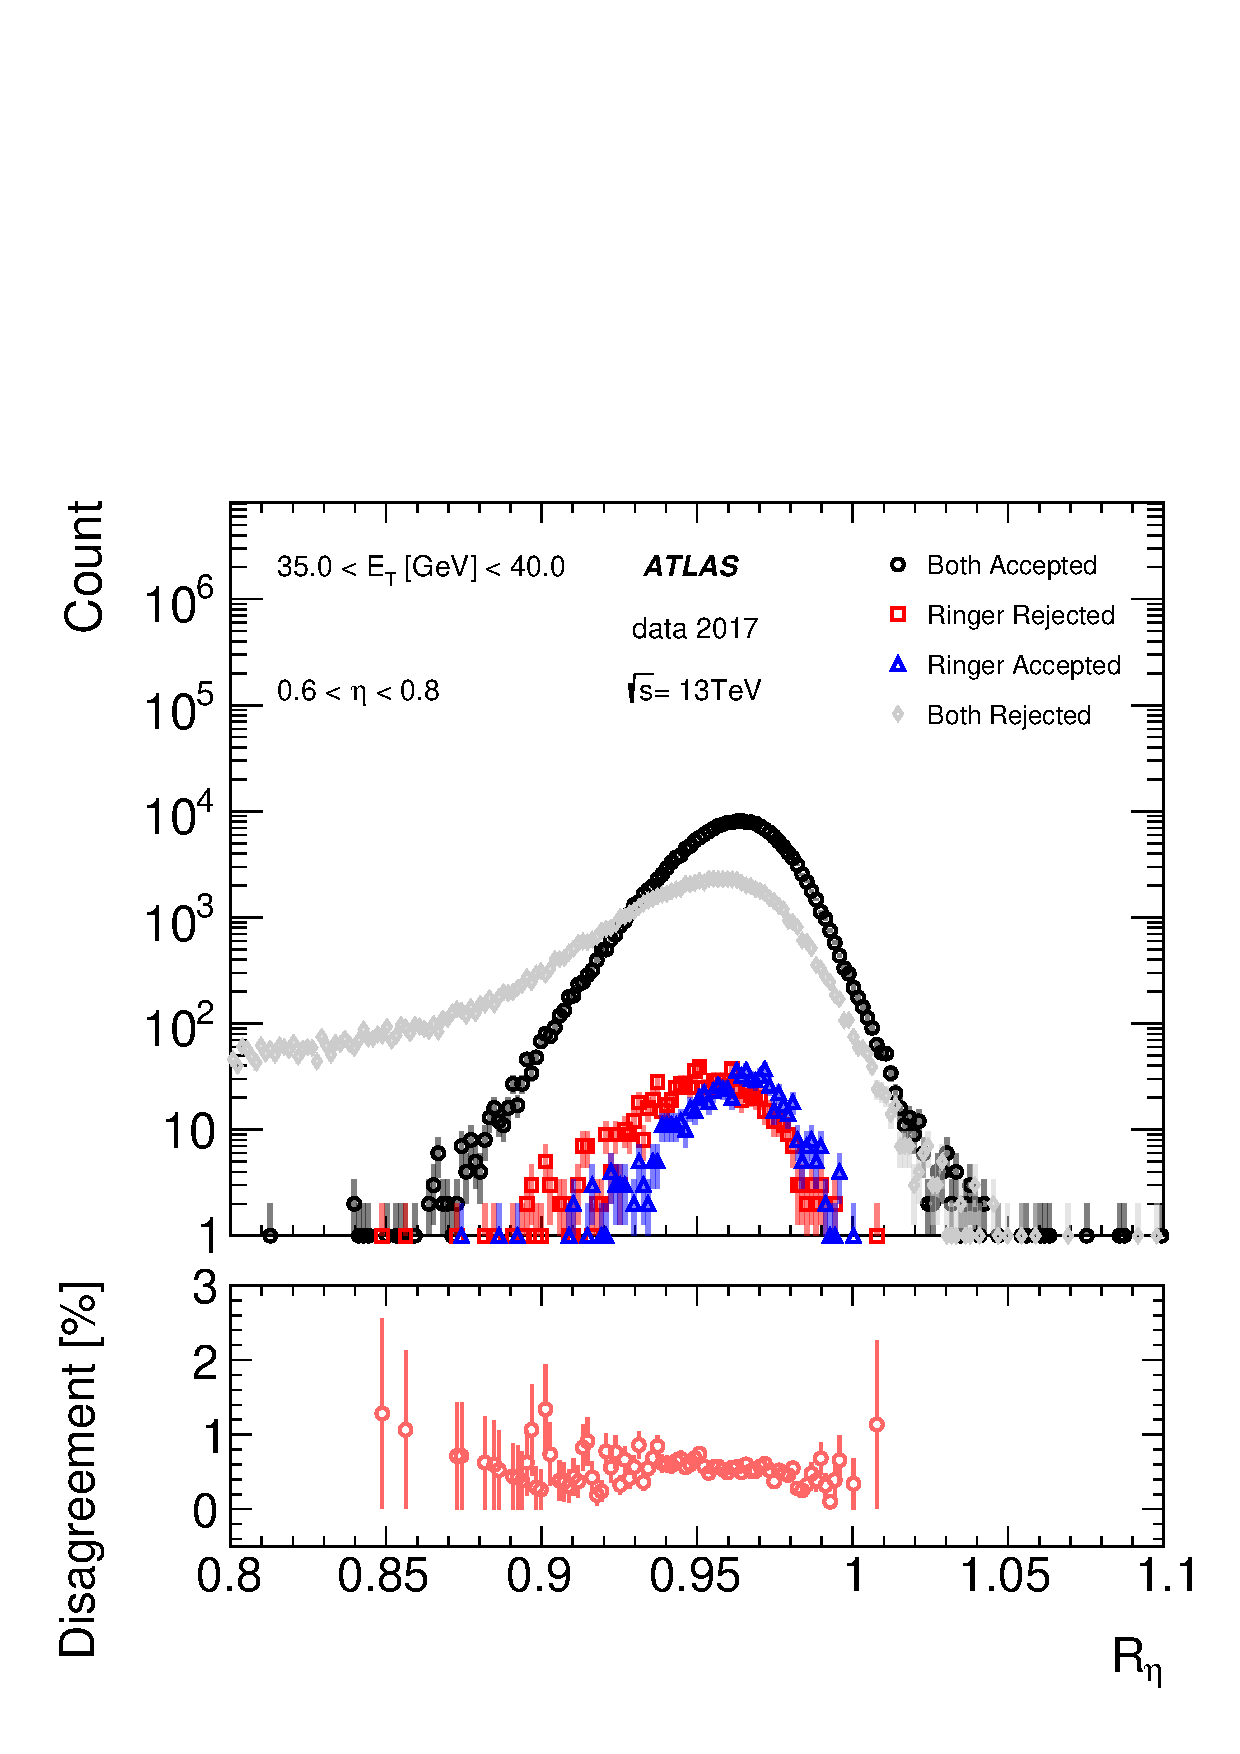
\includegraphics[width=\textwidth]{sections/04_analysis/figures/quadrant_plots/reta.pdf}
\caption{}
\label{fig:quadrant_calo_variables_30GeV_eta}
\end{subfigure}
%\hfill
\begin{subfigure}[c]{.49\textwidth}
\centering
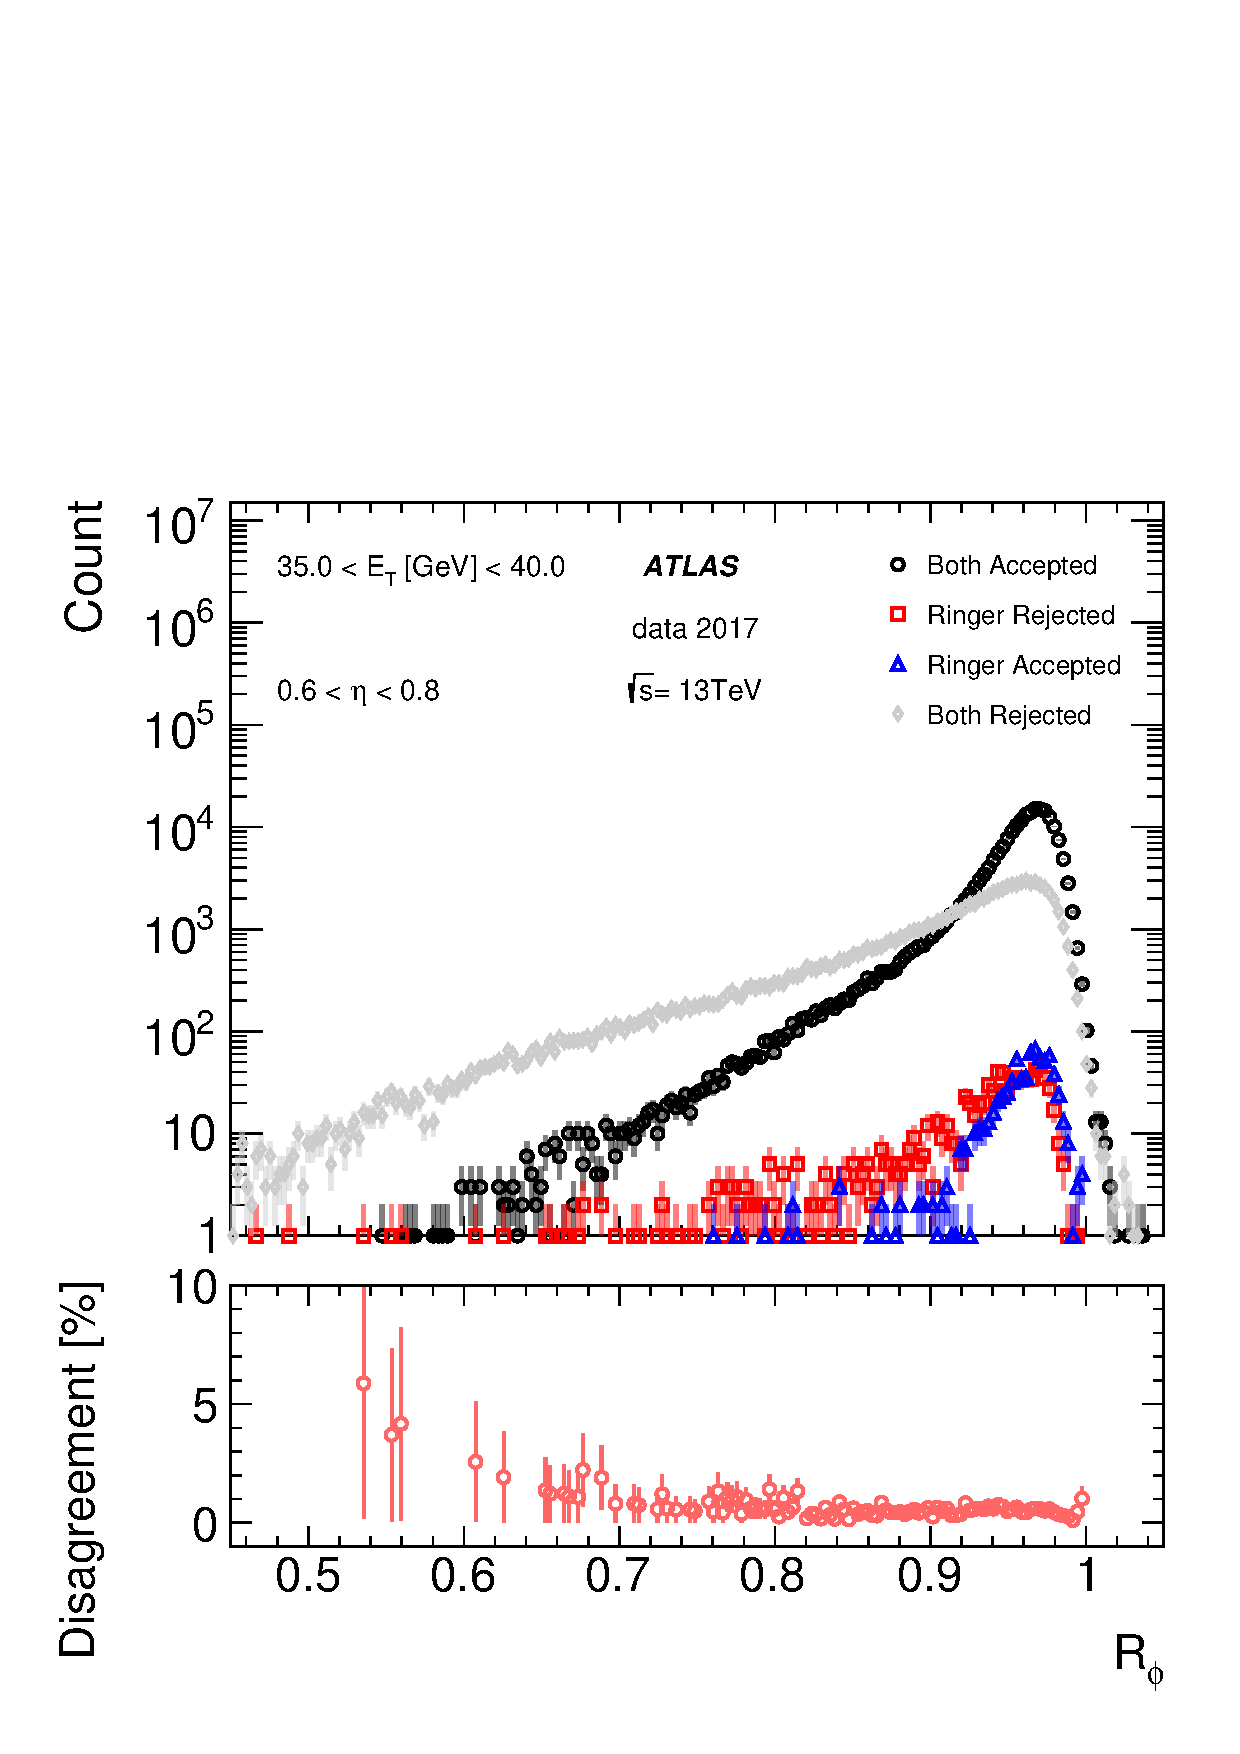
\includegraphics[width=\textwidth]{sections/04_analysis/figures/quadrant_plots/rphi.pdf}
\caption{}
\end{subfigure} 
%\end{figure}
%\begin{figure}[p]\ContinuedFloat
\begin{subfigure}[c]{.49\textwidth}
\centering
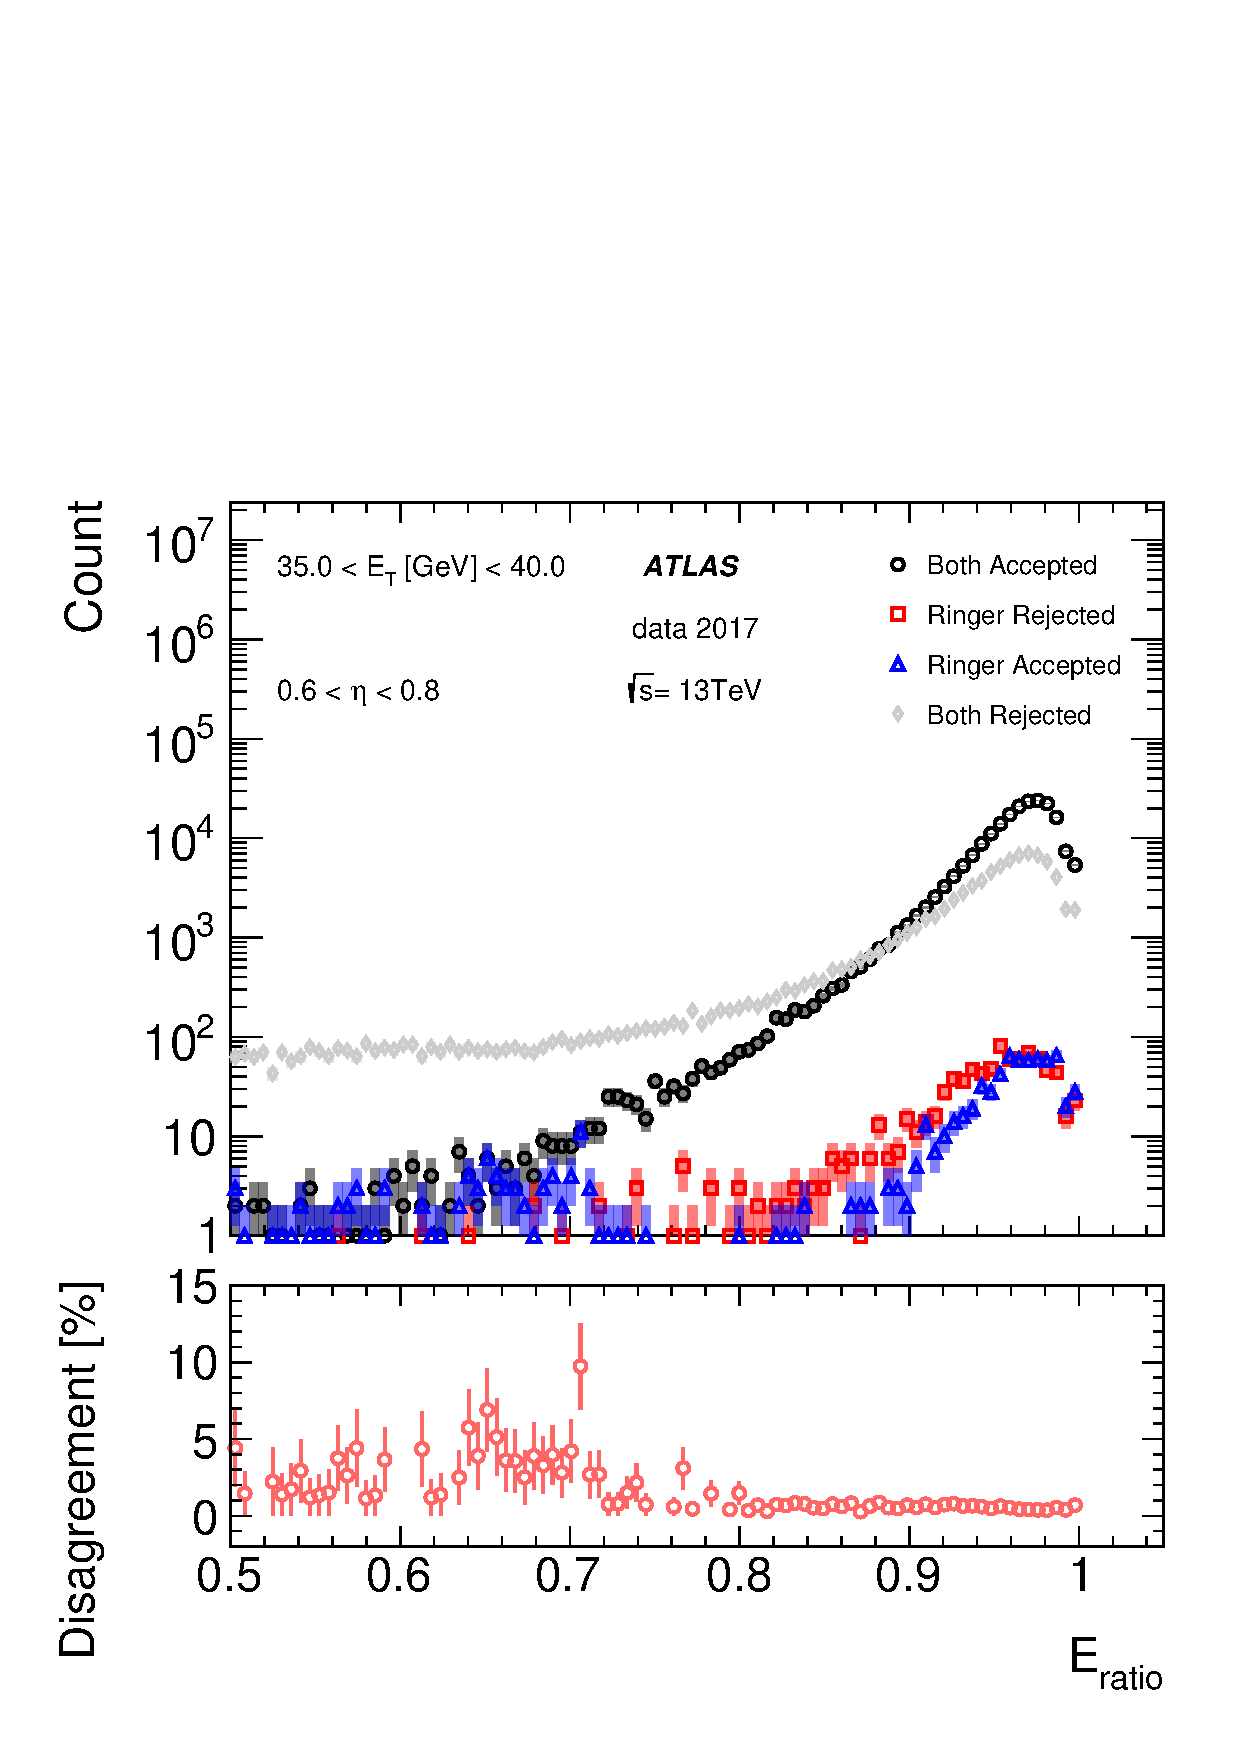
\includegraphics[width=\textwidth]{sections/04_analysis/figures/quadrant_plots/eratio.pdf}
\caption{}
\end{subfigure}
\hfill
\begin{subfigure}[c]{.49\textwidth}
\centering
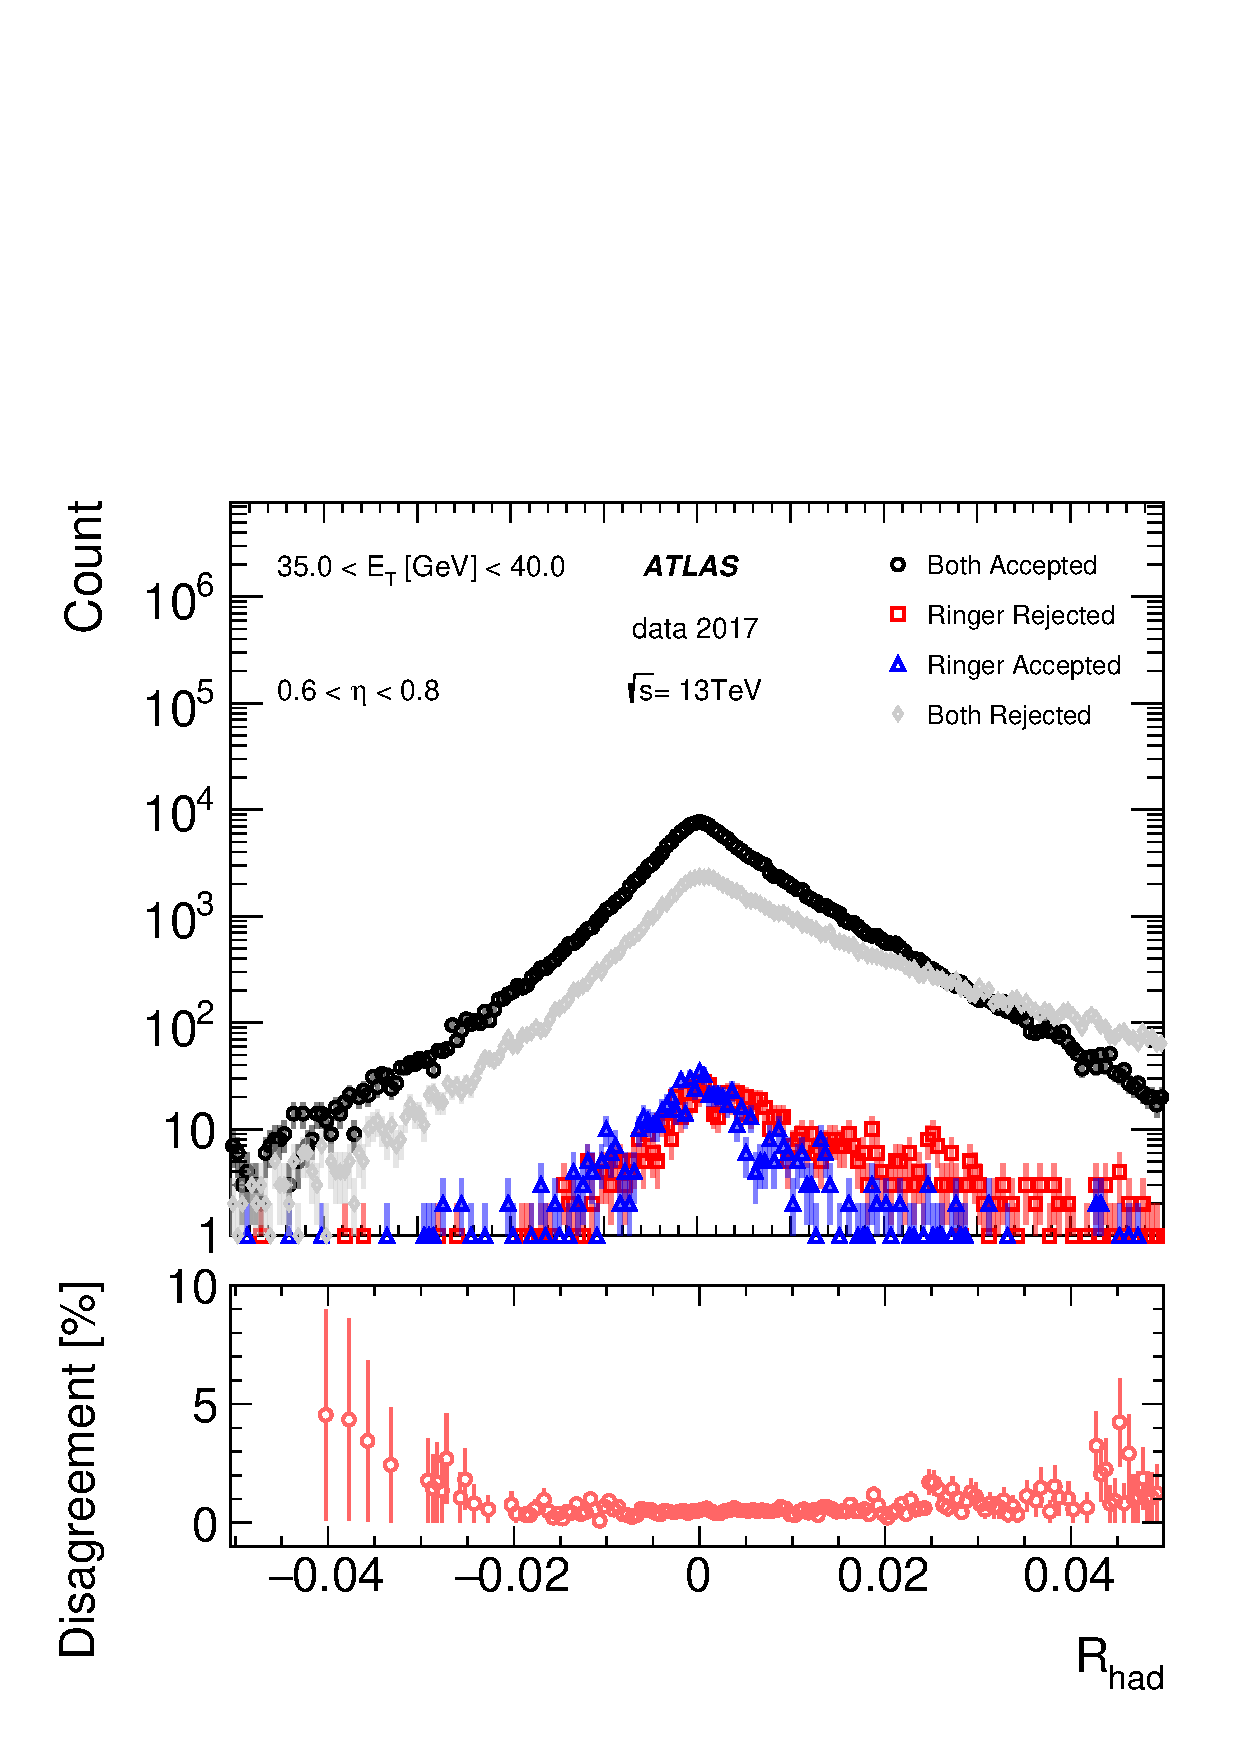
\includegraphics[width=\textwidth]{sections/04_analysis/figures/quadrant_plots/rhad.pdf}
\caption{}
\end{subfigure} \\


\caption{\label{fig:quadrant_calo_variables_30GeV}
	Quadrant \DIFdelbeginFL \DIFdelFL{analysis }\DIFdelendFL \DIFaddbeginFL \DIFaddFL{Analysis }\DIFaddendFL plots for the main offline-reconstructed
	calorimetry variables employed in the
	likelihood and for the $0.6<\abseta{}<0.8$ and
	\DIFdelbeginFL \DIFdelFL{$30<\et{}~[\text{GeV}]<35$ }\DIFdelendFL \DIFaddbeginFL \DIFaddFL{$30<\et{}<35$~}\GeV \DIFaddendFL region. 
	The top pad in each figure shows the raw number of \DIFdelbeginFL \DIFdelFL{observations }\DIFdelendFL \DIFaddbeginFL \DIFaddFL{candidates }\DIFaddendFL for the four mutually exclusive cases: \DIFaddbeginFL \DIFaddFL{accepted }\DIFaddendFL both with and without 
	\DIFaddbeginFL \DIFaddFL{the }\DIFaddendFL \rnn{} \DIFdelbeginFL \DIFdelFL{triggered }\DIFdelendFL (black); \DIFdelbeginFL \DIFdelFL{triggered }\DIFdelendFL \DIFaddbeginFL \DIFaddFL{accepted }\DIFaddendFL only with \DIFaddbeginFL \DIFaddFL{the }\DIFaddendFL \rnn{} (blue); \DIFdelbeginFL \DIFdelFL{triggered }\DIFdelendFL \DIFaddbeginFL \DIFaddFL{accepted }\DIFaddendFL only without \DIFaddbeginFL \DIFaddFL{the }\DIFaddendFL \rnn{} (red); \DIFdelbeginFL \DIFdelFL{neither one triggered }\DIFdelendFL \DIFaddbeginFL \DIFaddFL{rejected both with and without the }\rnn{} \DIFaddendFL (\DIFdelbeginFL \DIFdelFL{gray}\DIFdelendFL \DIFaddbeginFL \DIFaddFL{grey}\DIFaddendFL ). The bottom pad \DIFdelbeginFL \DIFdelFL{contains }\DIFdelendFL \DIFaddbeginFL \DIFaddFL{shows 
	the }\DIFaddendFL disagreement as defined in \DIFdelbeginFL \DIFdelFL{the Equation }\DIFdelendFL \DIFaddbeginFL \DIFaddFL{Eq.~}\DIFaddendFL \eqref{eq:disagreement}.
}
%Quadrant analysis plots for the offline-reconstructed
%calorimetry variables employed in the
%likelihood and \wstot{} for the $0.6<\abseta{}<0.8$ and
%$30<\et{}~[\text{GeV}]<40$ slices.}%
\end{figure}


\begin{comment}
    
\begin{figure}[h!tb]
%\centering
%\begin{subfigure}[c]{.49\textwidth}
\centering
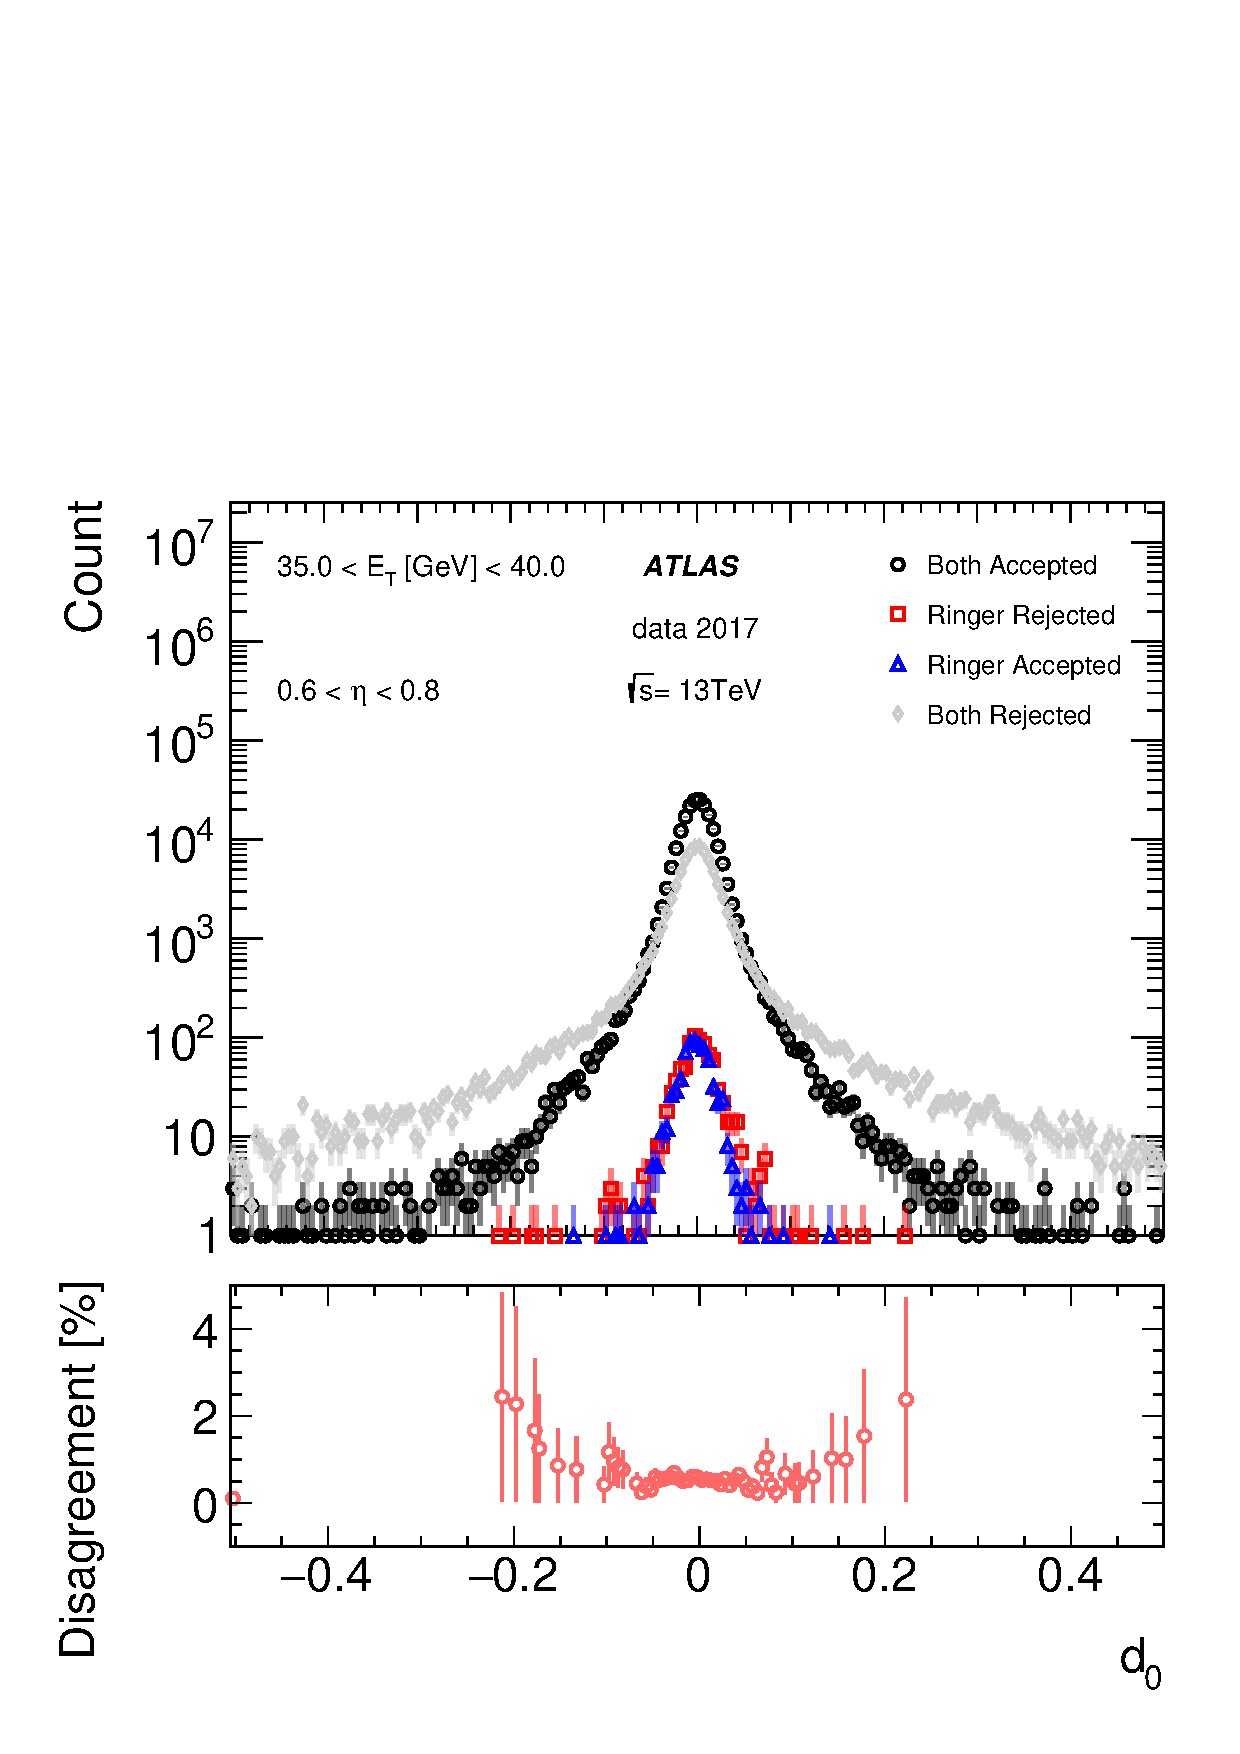
\includegraphics[width=.5\textwidth]{sections/04_analysis/figures/quadrant_plots/d0.pdf}
\caption{\label{fig:quadrant_track_variables_30GeV}
Quadrant analyses plots for the offline-reconstructed ID variable $d_0$ employed in the
likelihood for the $0.6<\abseta{}<0.8$ and $35<\et{}~[\text{GeV}]<40$ slice. The variable $d_0$ is defined as the transverse parameter of the impact point with respect to the collision beam.
}
\end{figure}
\end{comment}






\FloatBarrier
\subsection[Homogeneity Tests]{Homogeneity Tests}\label{ssec:agreement}

In this analysis, the impact \DIFaddbegin \DIFadd{on the likelihood algorithm }\DIFaddend of using different triggers, \rnn{} and cut-based, \DIFdelbegin \DIFdel{on the likelihood algorithm }\DIFdelend is evaluated. 
This study requires a pair of duplicated triggers, \DIFdelbegin \DIFdel{composed by an $E_T > 28$ }\DIFdelend \DIFaddbegin \DIFadd{applying an $\ET > 28$~}\DIFaddend GeV isolated and \DIFdelbegin \DIFdel{Tight }\DIFdelend \DIFaddbegin \enquote{tight} \DIFadd{electron }\DIFaddend selection with and without the \rnn{}, operating \DIFdelbegin \DIFdel{online together . 
This }\DIFdelend \DIFaddbegin \DIFadd{together online.  
The }\DIFaddend analysis is performed using \Zee{} \tnp{} collision data, which were selected with the trigger requirement set to either one of the duplicated \DIFaddbegin \DIFadd{online }\DIFaddend triggers for the tag, whereas the probe selection is invariably set to the offline \vloose{} criterion. This is \DIFdelbegin \DIFdel{the exact setup employed by ATLAS }\DIFdelend \DIFaddbegin \DIFadd{exactly the same set-up that ATLAS employed }\DIFaddend to derive the offline likelihood for electrons \DIFaddbegin \DIFadd{with }\ET \DIFaddend above \SI{15}{\GeV}~\cite{PERF-2017-01}. 
To benefit from the full 2017 \DIFdelbegin \DIFdel{statistics}\DIFdelend \DIFaddbegin \DIFadd{dataset}\DIFaddend , collision data collected \DIFdelbegin \DIFdel{previous to the }\DIFdelend \DIFaddbegin \DIFadd{before }\DIFaddend TS1 were also employed. \DIFdelbegin \DIFdel{In case }\DIFdelend \DIFaddbegin \DIFadd{If }\DIFaddend the profiles are statistically identical, \DIFdelbegin \DIFdel{then it is expected that }\DIFdelend the \rnn{} trigger \DIFdelbegin \DIFdel{does not }\DIFdelend \DIFaddbegin \DIFadd{is not expected to }\DIFaddend cause any relevant \DIFdelbegin \DIFdel{alteration }\DIFdelend \DIFaddbegin \DIFadd{change }\DIFaddend in the derivation of the offline likelihood \DIFdelbegin \DIFdel{pdfs}\DIFdelend \DIFaddbegin \DIFadd{PDFs}\DIFaddend .  
%The statistical method for profile evaluation is described in Section~\ref{top:homogeneity_method} and the results are available in Section~\ref{top:agreement_homogeneity_results}.




%\subsubsection{Method}\label{top:homogeneity_method}



The problem is \DIFdelbegin \DIFdel{approached based on homogeneity tests on }\DIFdelend \DIFaddbegin \DIFadd{addressed by applying homogeneity tests to }\DIFaddend histograms~\cite{homogeneity_test} \DIFdelbegin \DIFdel{, }\DIFdelend in order to check for systematic effects of the trigger configuration. \DIFdelbegin \DIFdel{It is }\DIFdelend \DIFaddbegin \DIFadd{These tests are }\DIFaddend based on a test originally developed by Pearson~\cite{pearson1911probability} and popularly employed in many fields beyond \DIFdelbegin \DIFdel{High Energy Physics (HEP)}\DIFdelend \DIFaddbegin \DIFadd{high-energy physics}\DIFaddend , e.g.\DIFaddbegin \DIFadd{\ }\DIFaddend social sciences~\cite{wickens2014multiway} and health~\cite{ma2015homogeneity}, \DIFdelbegin \DIFdel{usually labelled as }\DIFdelend \DIFaddbegin \DIFadd{where they are usually called }\DIFaddend contingency or consistency tests.

In order to benefit from the \DIFdelbegin \DIFdel{test }\DIFdelend \DIFaddbegin \DIFadd{tests }\DIFaddend without having to customize \DIFdelbegin \DIFdel{it to the ATLAS particular analysis setup}\DIFdelend \DIFaddbegin \DIFadd{them to an ATLAS-specific analysis set-up}\DIFaddend , the collision data \DIFdelbegin \DIFdel{was }\DIFdelend \DIFaddbegin \DIFadd{were }\DIFaddend split into two
statistically independent groups\DIFdelbegin \DIFdel{attempting to keep data taking }\DIFdelend \DIFaddbegin \DIFadd{, consisting of data alternately taken from consecutive short time periods to keep their data-taking }\DIFaddend conditions as
similar as possible\DIFdelbegin \DIFdel{by successively taking data to each group from small
consecutive periods}\DIFdelend . 

The \DIFdelbegin \DIFdel{p-value}\DIFdelend \DIFaddbegin \DIFadd{$p$-value}\DIFaddend , or probability value, is a measure used in statistical hypothesis testing to determine the significance of \DIFdelbegin \DIFdel{your }\DIFdelend \DIFaddbegin \DIFadd{one's }\DIFaddend results. It represents the probability of obtaining an observed result, or something more extreme\DIFaddbegin \DIFadd{, }\DIFaddend if the null hypothesis (which states that there is no effect or no difference) is true. By comparing the \DIFdelbegin \DIFdel{p-values }\DIFdelend \DIFaddbegin \DIFadd{$p$-values }\DIFaddend of the two groups, it is possible to evaluate how the different configurations affect the likelihood \DIFdelbegin \DIFdel{of the profiles }\DIFdelend \DIFaddbegin \DIFadd{that the profiles are }\DIFaddend being drawn from the same distribution.  If the \DIFdelbegin \DIFdel{p-values }\DIFdelend \DIFaddbegin \DIFadd{$p$-values }\DIFaddend have negligible fluctuations with respect to the values obtained \DIFdelbegin \DIFdel{by the }\DIFdelend \DIFaddbegin \DIFadd{from }\DIFaddend tests comparing the same triggers, then the systematic effect in the profiles is negligible \DIFdelbegin \DIFdel{with respect to half}\DIFdelend \DIFaddbegin \DIFadd{for a dataset that is half}\DIFaddend \footnote{\DIFdelbegin \DIFdel{Once each }\DIFdelend \DIFaddbegin \DIFadd{Each }\DIFaddend group \DIFdelbegin \DIFdel{is using nearly }\DIFdelend \DIFaddbegin \DIFadd{contains approximately }\DIFaddend half of the integrated luminosity.} of the \DIFdelbegin \DIFdel{statistics available }\DIFdelend \DIFaddbegin \DIFadd{size of the whole available dataset}\DIFaddend .

%\footnote{The p-value here is defined by: $P-value \approx f(x, k) = \frac{1}{2^{k/2}\Gamma(k/2)}x^{k/2 -1}e^{-x/2}$, where $x\in(0, \infty)$ and $k>0$}

To provide \DIFdelbegin \DIFdel{a better insight on }\DIFdelend \DIFaddbegin \DIFadd{better insight into }\DIFaddend possible distortions, the corresponding 
\DIFdelbegin \DIFdel{$\chi$
individual }\DIFdelend \DIFaddbegin \DIFadd{individual $\chi$ }\DIFaddend contributions of each group are computed\DIFaddbegin \DIFadd{, }\DIFaddend allowing them to 
\DIFdelbegin \DIFdel{freely
oscillate through the positive and negative axis with
}\DIFdelend \DIFaddbegin \DIFadd{assume positive or negative values by defining
}\DIFaddend 

\begin{equation}
  \chi_{i,j}^{s} = \frac{(r_{i,j} - b_{i,j})}{\sqrt{b_{i,j}}},
  \label{eq:signed_chi}
\end{equation}

\noindent where $r_{i,j}$ ($b_{i,j}$) is the number of observations collected by
the trigger with (without) \DIFaddbegin \DIFadd{the }\DIFaddend \rnn{} in \DIFdelbegin \DIFdel{$j$th }\DIFdelend \DIFaddbegin \DIFadd{$j^\text{th}$ }\DIFaddend histogram bin and in the \DIFdelbegin \DIFdel{$i$th
}\DIFdelend \DIFaddbegin \DIFadd{$i^\text{th}$
}\DIFaddend $\et{}\times\abseta{}$ region.


\subsubsection{Results}\label{top:agreement_homogeneity_results}




Regardless the trigger configuration, the \DIFdelbegin \DIFdel{p-values of the }\DIFdelend homogeneity tests between the two groups result in similar \DIFdelbegin \DIFdel{values}\DIFdelend \DIFaddbegin \DIFadd{$p$-values}\DIFaddend . In other words, the fluctuations in the profiles are mainly \DIFdelbegin \DIFdel{dominated by statisticalfluctuations}\DIFdelend \DIFaddbegin \DIFadd{statistical}\DIFaddend , with no sign of systematic effects due to the trigger configuration. 

\DIFdelbegin \DIFdel{A similar behavior is observed for the ID and calo-ID variables. The }\DIFdelend Figure~\ref{fig:groups_homogeneity_calo} shows the residuals \DIFdelbegin \DIFdel{when considering the histogram obtained with }\DIFdelend \DIFaddbegin \DIFadd{for the }\reta\DIFadd{, }\rphi\DIFadd{, }\eratio\DIFadd{, and }\rhad \DIFadd{calorimetry variables when the reference histogram is obtained from }\DIFaddend collision data collected by the trigger without \DIFaddbegin \DIFadd{the }\DIFaddend \rnn{} for the first \DIFdelbegin \DIFdel{arbitrary groupas a reference}\DIFdelend \DIFaddbegin \DIFadd{group}\DIFaddend . The residuals are dominated by statistical fluctuations, \DIFdelbegin \DIFdel{which }\DIFdelend \DIFaddbegin \DIFadd{and }\DIFaddend are within the expectations from \DIFaddbegin \DIFadd{the }\DIFaddend homogeneity hypothesis for most variables and regions. \DIFaddbegin \DIFadd{Similar behaviour is observed for track variables. 
}\DIFaddend 

\begin{figure}[h!]
\begin{center}
\begin{subfigure}[c]{.48\textwidth}
\centering
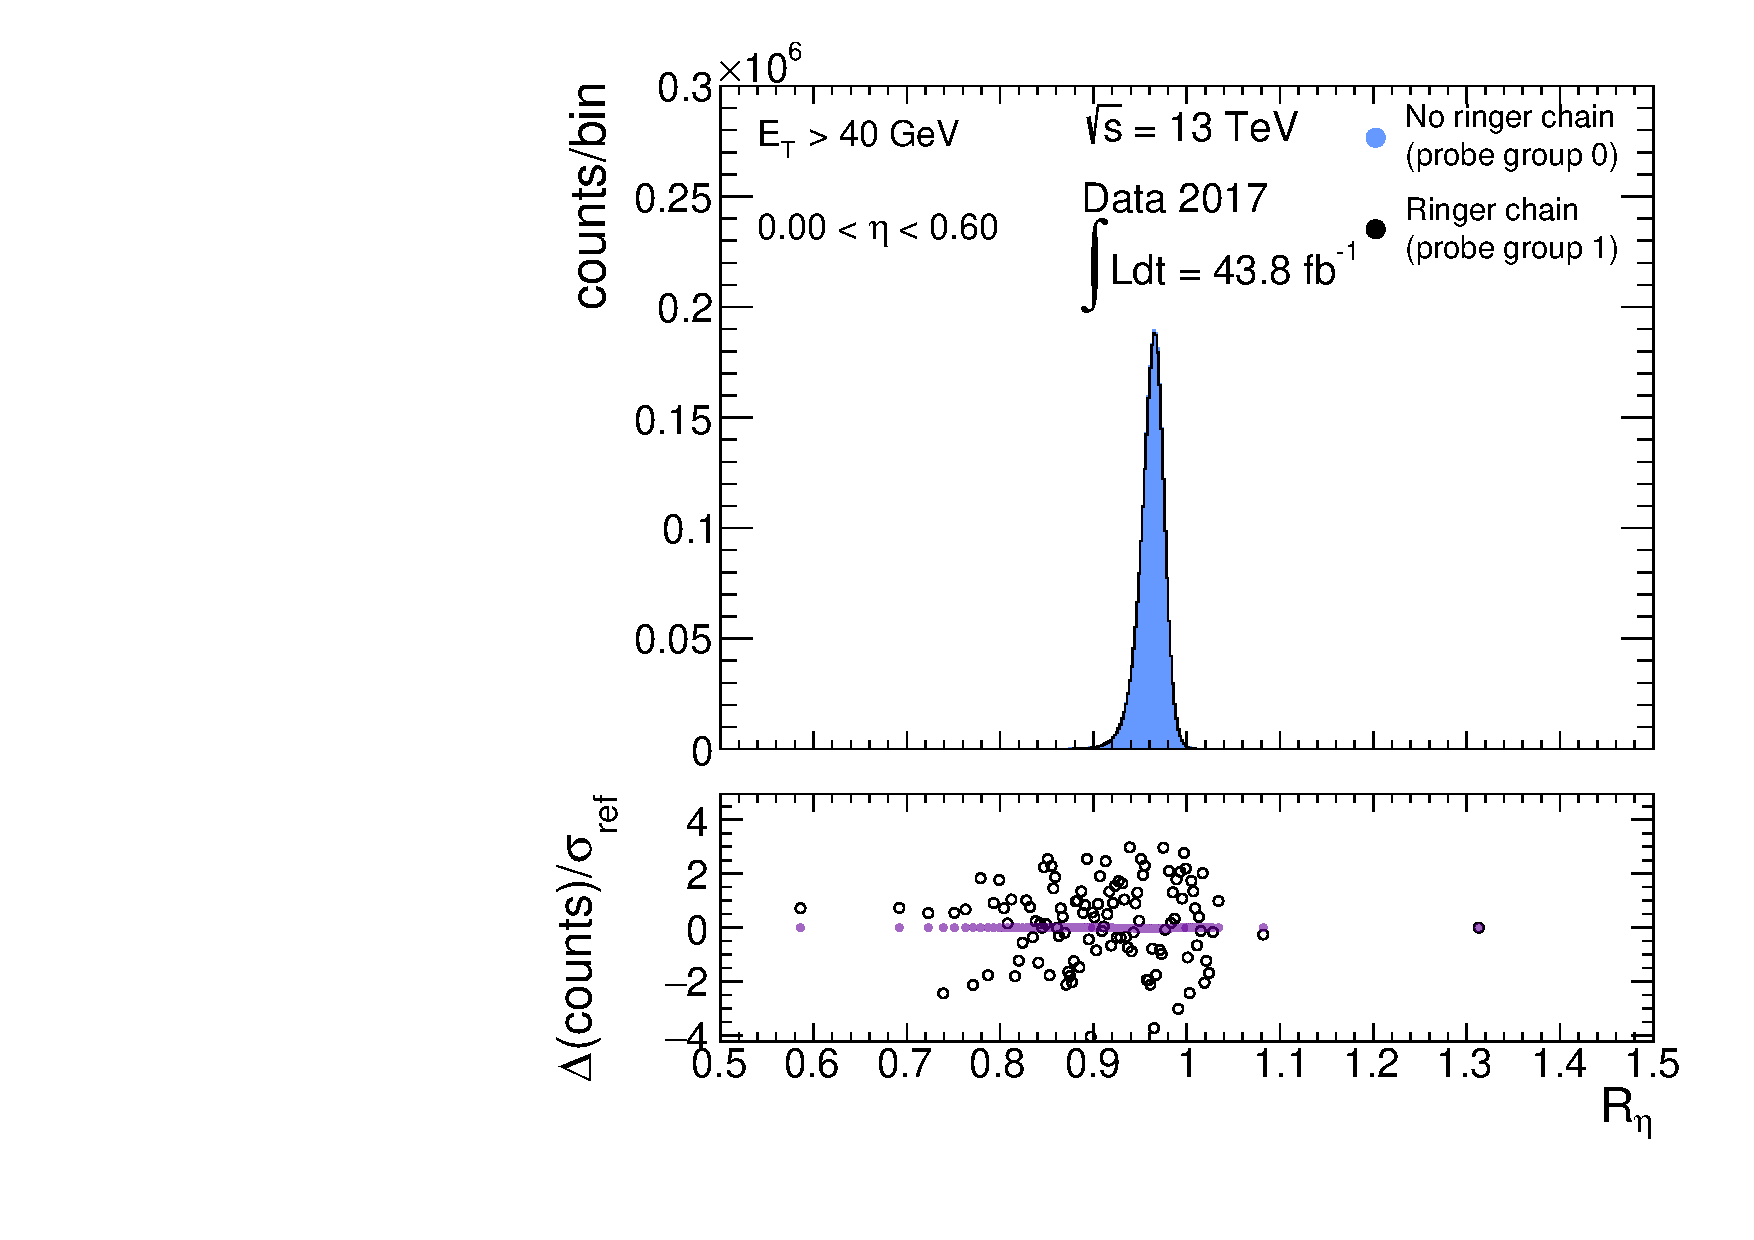
\includegraphics[width=\textwidth]{sections/04_analysis/figures/noAdjustment/el_reta_et40eta0_00_sigma_base_new.pdf}
\caption{}%

\end{subfigure}
\hfill
\begin{subfigure}[c]{.48\textwidth}
\centering
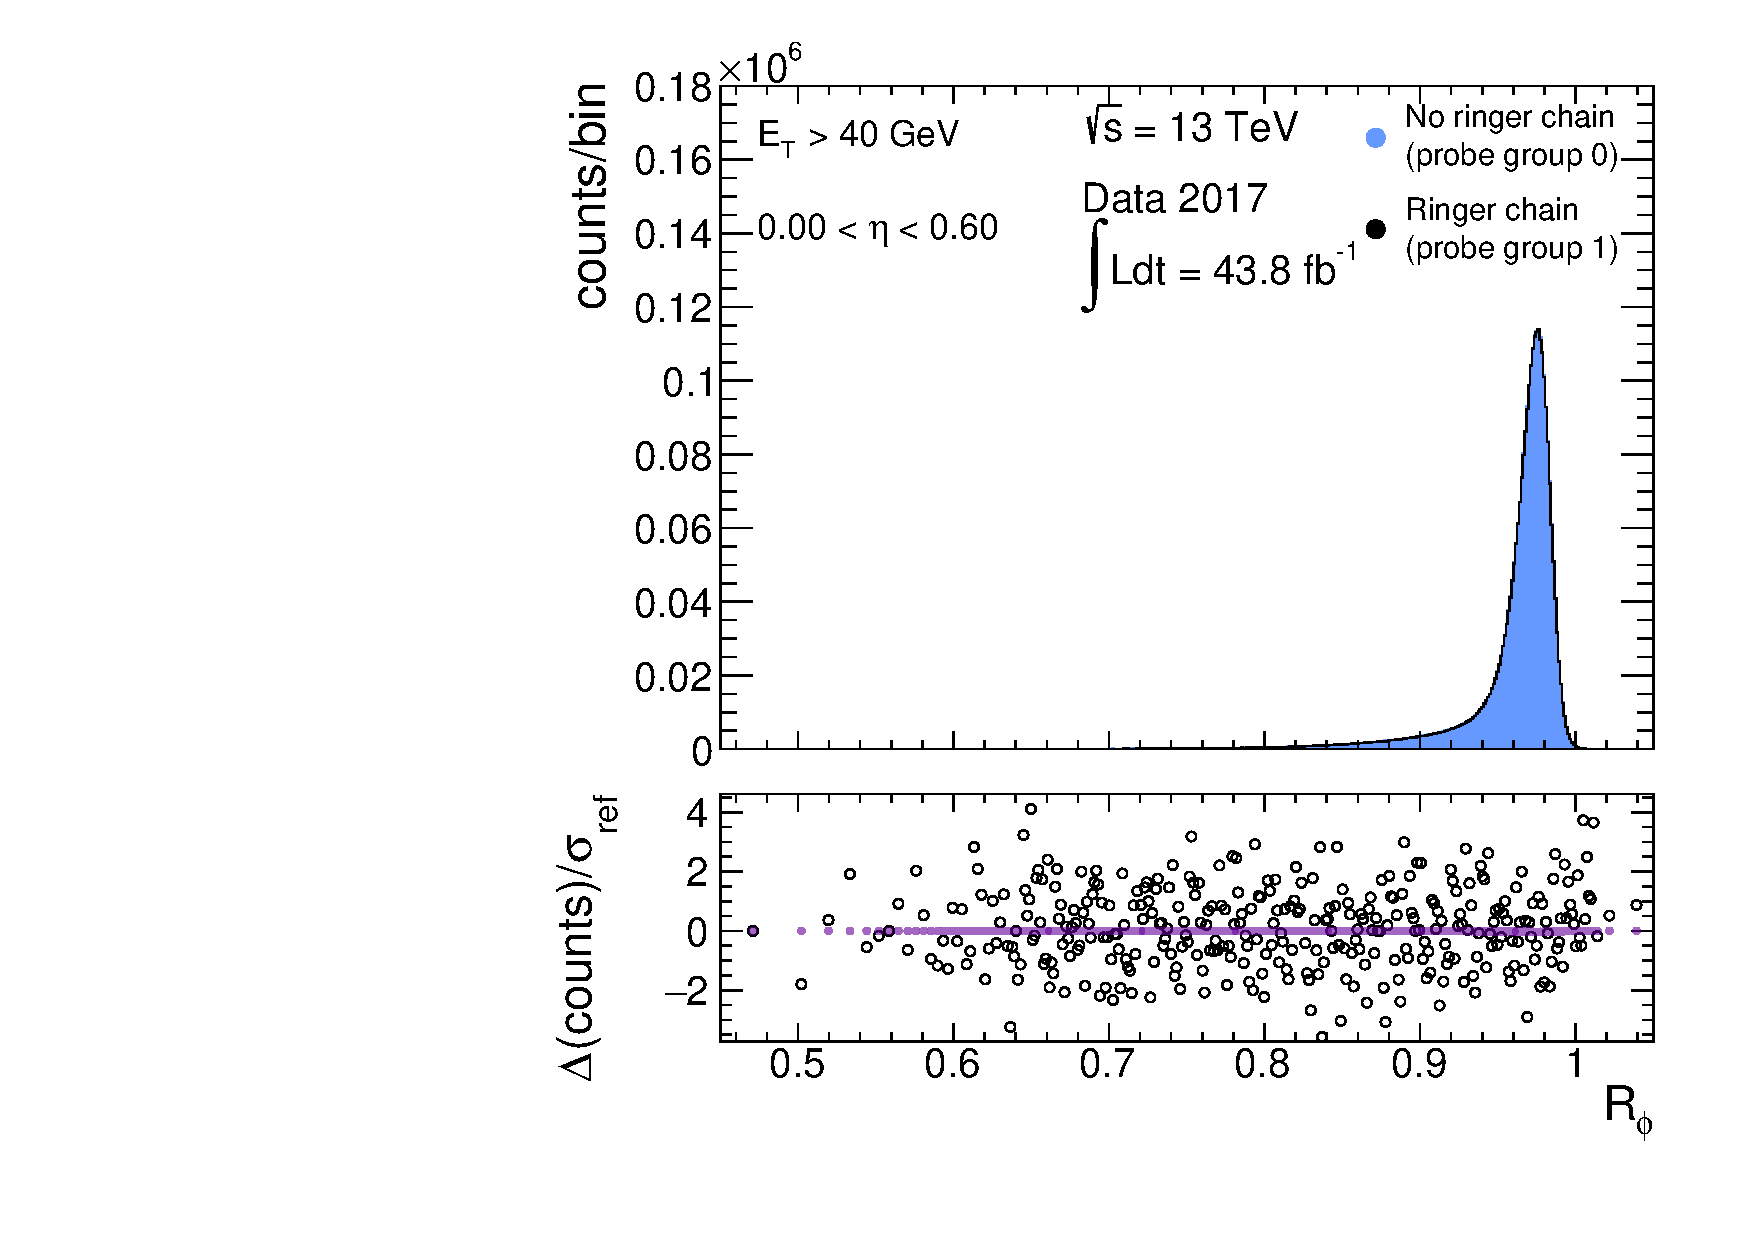
\includegraphics[width=\textwidth]{sections/04_analysis/figures/noAdjustment/el_rphi_et40eta0_00_sigma_base_new.pdf}
\caption{}%

\end{subfigure} \\
\begin{subfigure}[c]{.48\textwidth}
\centering
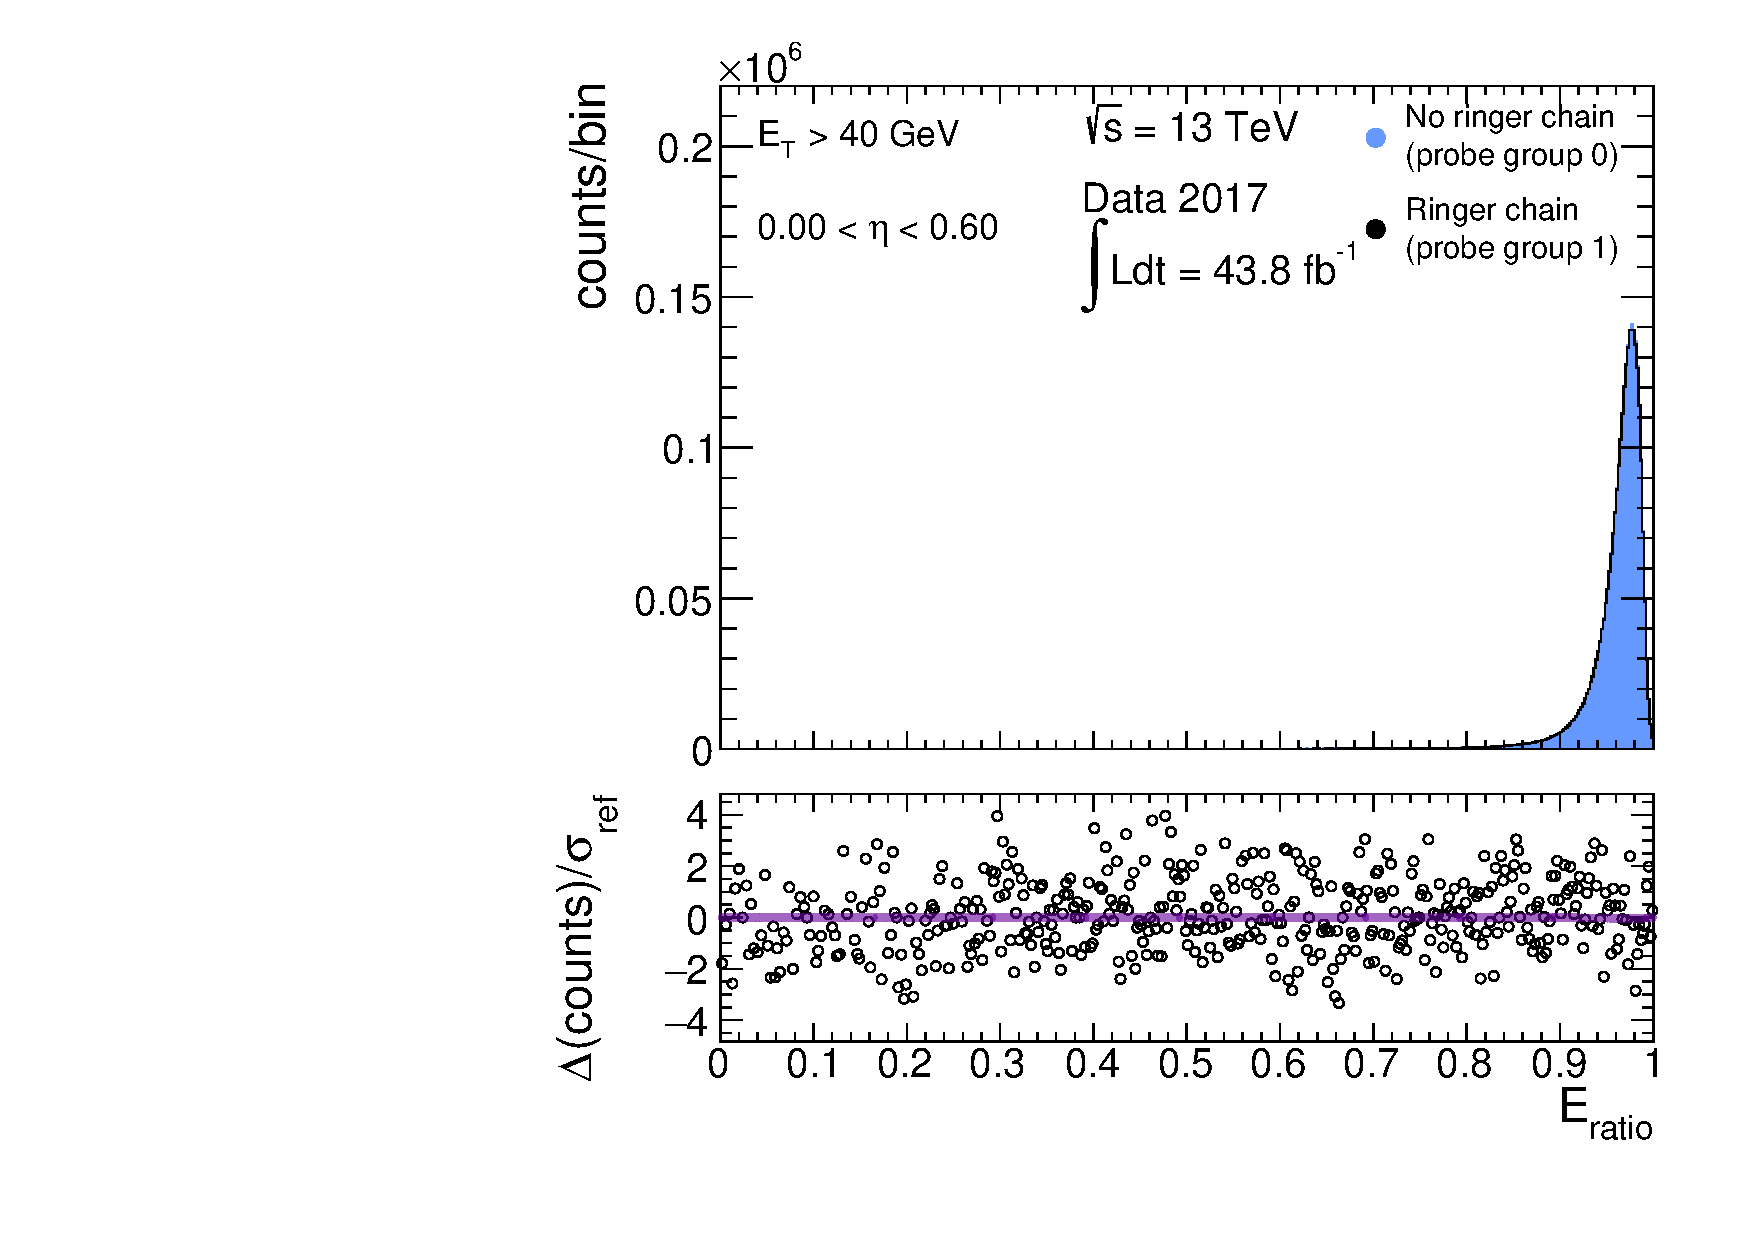
\includegraphics[width=\textwidth]{sections/04_analysis/figures/noAdjustment/el_eratio_et40eta0_00_sigma_base_new.pdf}
\caption{}%

\end{subfigure}
\hfill
\begin{subfigure}[c]{.48\textwidth}
\centering
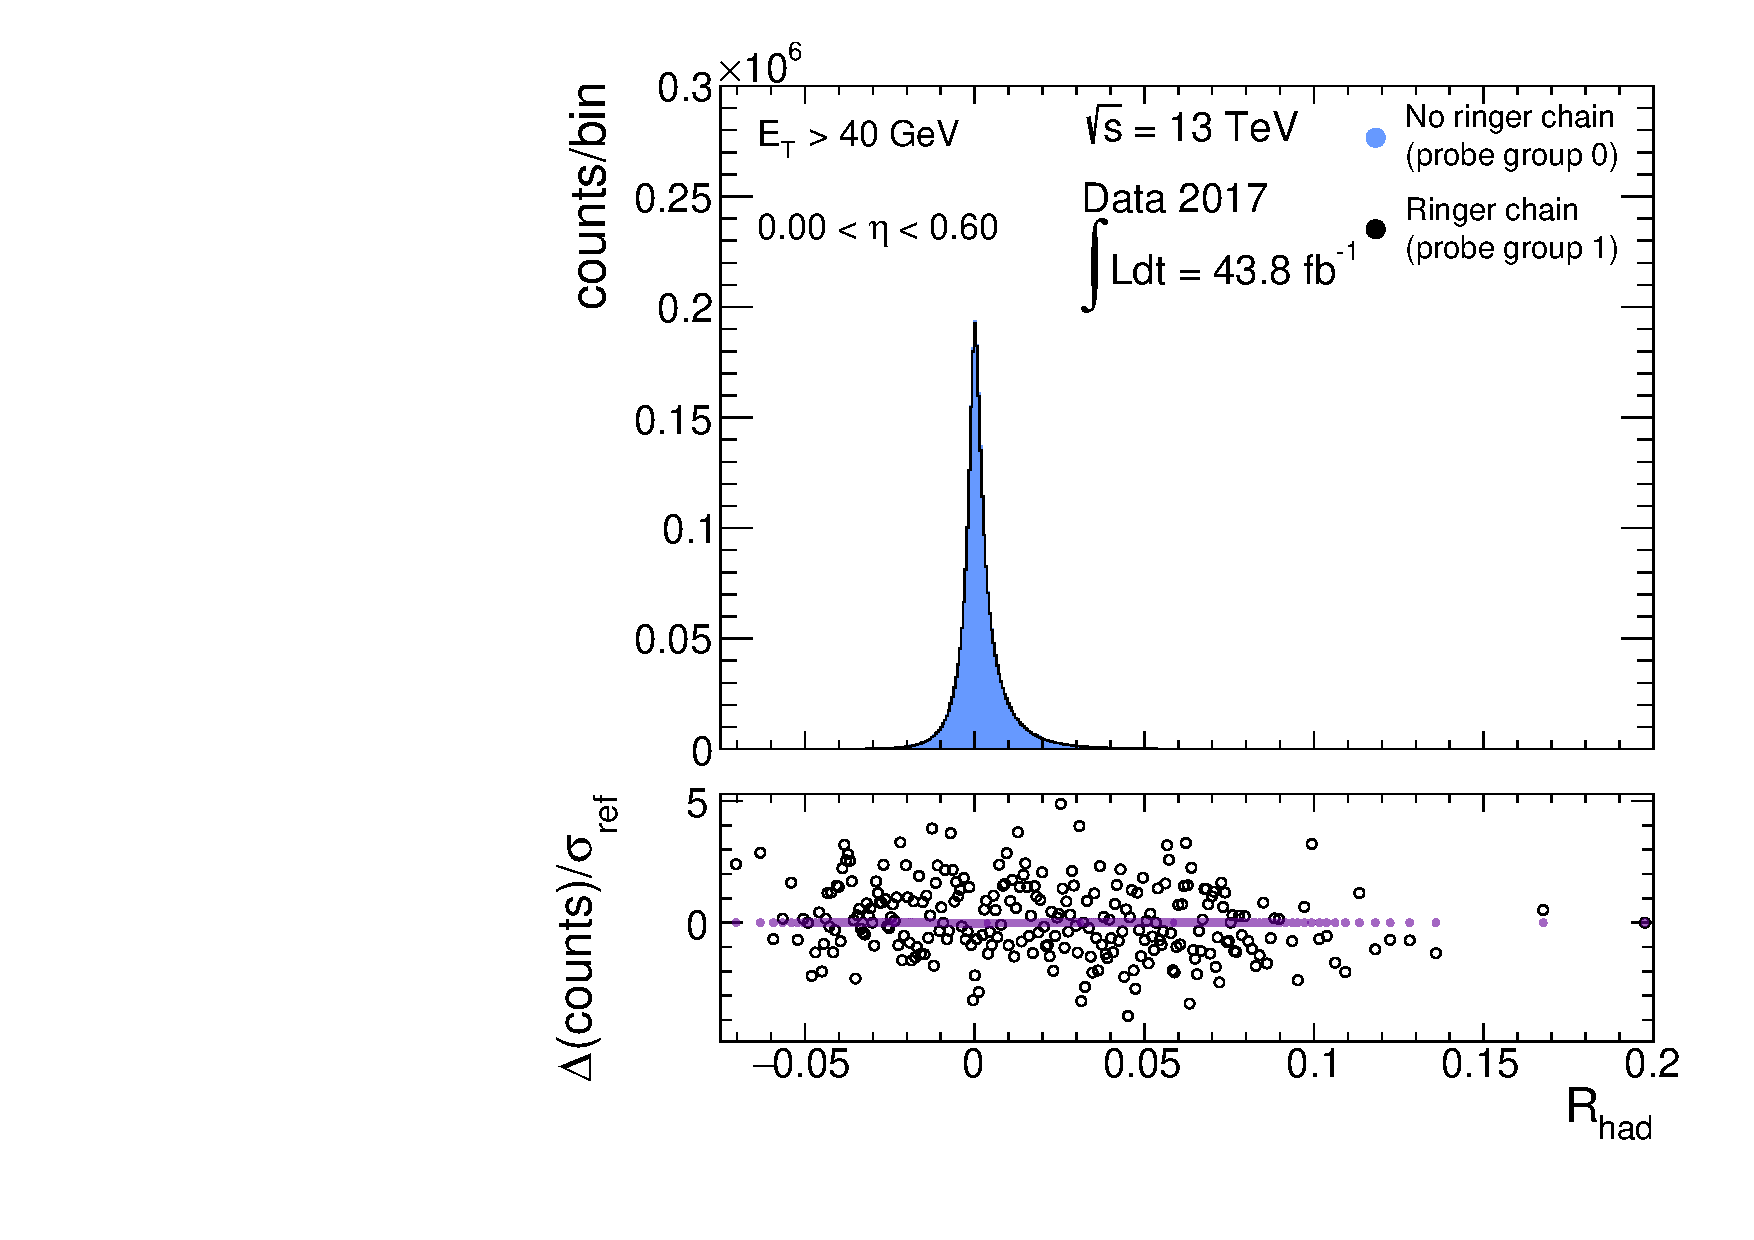
\includegraphics[width=\textwidth]{sections/04_analysis/figures/noAdjustment/el_rhad_et40eta0_00_sigma_base_new.pdf}
\caption{}%

\end{subfigure} \\
\caption{%
	Top: \DIFaddbeginFL \DIFaddFL{Profile histograms for the }\DIFaddendFL \reta, \DIFdelbeginFL %DIFDELCMD < \eratio%%%
\DIFdelFL{, }\DIFdelendFL \rphi, \DIFaddbeginFL \eratio\DIFaddFL{, and }\DIFaddendFL \rhad \DIFdelbeginFL \DIFdelFL{histogram profiles for the }\DIFdelendFL calorimetry variables employed 
	in the offline likelihood in the $\et>\SI{40}{\GeV}$ and \DIFdelbeginFL \DIFdelFL{$0.00<\abseta{}<0.80$ }\DIFdelendFL \DIFaddbeginFL \DIFaddFL{$0.0<\abseta{}<0.8$ }\DIFaddendFL regions using 
	collision data collected by triggering without \DIFaddbeginFL \DIFaddFL{the }\DIFaddendFL \rnn{} in the first arbitrary data group
	(blue area \DIFaddbeginFL \DIFaddFL{histogram}\DIFaddendFL ) and collision data collected by triggering with \DIFaddbeginFL \DIFaddFL{the }\DIFaddendFL \rnn{} in the second
	arbitrary data group (black line \DIFaddbeginFL \DIFaddFL{histogram}\DIFaddendFL ).  Bottom: residual contributions using 
	\DIFdelbeginFL \DIFdelFL{as
	statistics }\DIFdelendFL \DIFaddbeginFL \DIFaddFL{the }\DIFaddendFL $\chi^s$ \DIFaddbeginFL \DIFaddFL{statistic }\DIFaddendFL (\DIFdelbeginFL \DIFdelFL{equation}\DIFdelendFL \DIFaddbeginFL \DIFaddFL{black circles, from Eq.}\DIFaddendFL ~\DIFaddbeginFL \DIFaddFL{(}\DIFaddendFL \ref{eq:signed_chi}\DIFdelbeginFL \DIFdelFL{, in black}\DIFdelendFL )\DIFaddbeginFL \DIFaddFL{), }\DIFaddendFL and the expected
	\DIFdelbeginFL \DIFdelFL{model for no distortion given by the }\DIFdelendFL $\chi^s$ residuals \DIFdelbeginFL \DIFdelFL{w.r.t.}%DIFDELCMD < \@ %%%
\DIFdelendFL \DIFaddbeginFL \DIFaddFL{if there are no distortions or statistical fluctuations with respect to }\DIFaddendFL the
	reference \DIFaddbeginFL \DIFaddFL{(purple dots at zero)}\DIFaddendFL .
}%
\label{fig:groups_homogeneity_calo}
\end{center}
\end{figure}%


\FloatBarrier
 \newpage  % ok
 \newpage \section{Conclusion}\label{sec:conclusion}
%-------------------------------------------------------------------------------


% Comparison with standard strategies
The \rnn{} \DIFdelbegin \DIFdel{is }\DIFdelend \DIFaddbegin \DIFadd{has }\DIFaddend an innovative design for electron selection based on
calorimetry information. With the
\DIFdelbegin \DIFdel{ambition to comply with }\DIFdelend \DIFaddbegin \DIFadd{goal of satisfying }\DIFaddend specific trigger system demands, \DIFdelbegin \DIFdel{the feature extraction
of }\DIFdelend \DIFaddbegin \DIFadd{feature extraction
from }\DIFaddend concentric ring energy sums provides an efficient description, which is quickly derived through simple operations. 
\DIFdelbegin \DIFdel{Neural network }\DIFdelend \DIFaddbegin \DIFadd{Neural-network }\DIFaddend models are employed \DIFdelbegin \DIFdel{for exploiting
nonlinear }\DIFdelend \DIFaddbegin \DIFadd{to exploit non-linear }\DIFaddend correlations between rings\DIFdelbegin \DIFdel{and the optimisation }\DIFdelend \DIFaddbegin \DIFadd{, and the optimization }\DIFaddend of this strategy 
culminated in the \DIFdelbegin \DIFdel{employment }\DIFdelend \DIFaddbegin \DIFadd{deployment }\DIFaddend of a set of \DIFdelbegin \DIFdel{specialist models per regions }\DIFdelend \DIFaddbegin \DIFadd{models specific to each region }\DIFaddend of pseudorapidity and transverse energy. 


In the second half of 2017, the \rnn{} algorithm replaced \DIFdelbegin \DIFdel{such }\DIFdelend a cut-based strategy
in the \fastcalo{} decision step \DIFaddbegin \DIFadd{of the }\hlt{} \DIFaddend and became the baseline algorithm
for triggering events containing electrons \DIFaddbegin \DIFadd{with }\ET \DIFaddend above \SI{15}{\GeV}, 
as part of the ATLAS online system\DIFdelbegin \DIFdel{CPU }\DIFdelend \DIFaddbegin \DIFadd{'s CPU-time }\DIFaddend reduction campaign. 
\DIFdelbegin \DIFdel{furthermore }\DIFdelend \DIFaddbegin \DIFadd{Furthermore, }\DIFaddend it was the first time a \DIFdelbegin \DIFdel{neural network }\DIFdelend \DIFaddbegin \DIFadd{neural-network }\DIFaddend method was employed as a 
baseline \DIFdelbegin \DIFdel{selection algorithm for event selection }\DIFdelend \DIFaddbegin \DIFadd{event-selection algorithm }\DIFaddend in the ATLAS trigger system.


During 2017 operation, \DIFdelbegin \DIFdel{based on neural networks trained with }\DIFdelend \DIFaddbegin \DIFadd{with the }\rnn{} \DIFadd{algorithm trained on }\DIFaddend simulated data, 
\DIFdelbegin \DIFdel{a
reduction factors }\DIFdelend \DIFaddbegin \DIFadd{fake-electron trigger rates were reduced by a factor }\DIFaddend of 13 in the \fastcalo{} \DIFdelbegin \DIFdel{and }\DIFdelend \DIFaddbegin \DIFadd{step 
and by a factor }\DIFaddend of 2 \DIFaddbegin \DIFadd{overall }\DIFaddend in the \hlt{} \DIFdelbegin \DIFdel{of fake rates were achieved }\DIFdelend with respect to the offline likelihood \DIFdelbegin \DIFdel{, while
keeping high electron efficiency similar to lowest energy-threshold unprescaled single electron trigger}\DIFdelend \DIFaddbegin \DIFadd{algorithm, while
achieving high electron-selection efficiencies very similar to those of relevant single-electron triggers without the }\rnn{}\DIFaddend . 
For 2018, the \rnn{} was trained with collision
data\DIFaddbegin \DIFadd{, }\DIFaddend resulting in an estimated additional reduction factor of 1.19--1.69 \DIFaddbegin \DIFadd{for fake-electron triggers }\DIFaddend in the \fastcalo{} \DIFaddbegin \DIFadd{step }\DIFaddend with respect to 2017. 
\DIFdelbegin \DIFdel{Additionally, the }\DIFdelend \DIFaddbegin \DIFadd{The }\DIFaddend \rnn{} was also studied \DIFdelbegin \DIFdel{through the }\DIFdelend \DIFaddbegin \DIFadd{from an }\DIFaddend offline likelihood perspective to \DIFdelbegin \DIFdel{bring additional insights on its behavior }\DIFdelend \DIFaddbegin \DIFadd{obtain additional insights into its behaviour by }\DIFaddend using two equivalent \DIFdelbegin \DIFdel{single electron trigger }\DIFdelend \DIFaddbegin \DIFadd{single-electron triggers }\DIFaddend with and without the \rnn{}. The \DIFdelbegin \DIFdel{proposed quadrant analysis allowed to observe high agreement between both triggerswith slight shifts }\DIFdelend \DIFaddbegin \enquote{quadrant analysis} \DIFadd{showed a high level of agreement between the two triggers, with the }\rnn{} \DIFadd{trigger showing a slight bias }\DIFaddend towards the signal region in the disagreement profiles of some calorimetry-based variables. Finally, \DIFdelbegin \DIFdel{when considering homogeneity test, the p-values of the }\DIFdelend \DIFaddbegin \DIFadd{the }\enquote{homogeneity tests} \DIFaddend between the two groups \DIFdelbegin \DIFdel{result in similar values}\DIFdelend \DIFaddbegin \DIFadd{of data resulted in similar $p$-values}\DIFaddend . In other words, the fluctuations in the profiles are mainly \DIFdelbegin \DIFdel{dominated by statisticalfluctuations}\DIFdelend \DIFaddbegin \DIFadd{statistical}\DIFaddend , with no sign of systematic effects due to the trigger configuration.



Physics beyond the Standard Model is getting more attention at the LHC and is expected to be part of the main focus in the data-taking phases to
come. At the beginning of \DIFdelbegin \DIFdel{Run~3}\DIFdelend \DIFaddbegin \RunThr\DIFaddend , the \rnn was updated to \DIFdelbegin \DIFdel{comprise closer-by electron (}\DIFdelend \DIFaddbegin \DIFadd{include events in which electrons have smaller angular separations (such as in }\DIFaddend boosted topologies)\DIFdelbegin \DIFdel{events}\DIFdelend , particularly limiting the effect of other contributions at
the edge of the feature extraction window, which can result from these physics
processes. In addition, \DIFdelbegin \DIFdel{an extension to }\DIFdelend \DIFaddbegin \DIFadd{the }\DIFaddend \rnn \DIFaddbegin \DIFadd{was extended into the }\ET \DIFadd{region }\DIFaddend below 15\DIFdelbegin \DIFdel{GeV was implemented }\DIFdelend \DIFaddbegin \DIFadd{~GeV, }\DIFaddend motivated by the high CPU \DIFdelbegin \DIFdel{demand of all }\DIFdelend \DIFaddbegin \DIFadd{demands of }\DIFaddend triggers in this kinematic region.





\begin{comment}



    


% Quadrant and agreement analysis
The \rnn{} was also studied through the offline likelihood perspective 
to bring additional insights on its behavior. By
taking advantage of the low dimensionality, low correlation and high
interpretability power of the variables employed in the likelihood, we derived
the profiles of the disjoint decision cases of the 2017 duplicate trigger pair.
The choice for the duplicated pair considered the typical scenario employed for
analysis with the setup that would maximize the disagreement between both
configurations: with and without the \rnn{}. The proposed quadrant analysis
allowed to observe high agreement between both triggers with slight shifts
towards the signal region in the disagreement profiles of some calorimetry-based
variables. By checking the agreement between the trigger pair for the derivation
of the likelihood pdfs, the alteration using the full 2017 data was much lower
than estimated statistical fluctuations. The residuals were found to be bounded
by \SI{0.2}{$\sigma$} for all variables. When considering only the
disagreement profiles, homogeneity hypothesis at a \SI{5}{\%} level was not
rejected for the calorimetry variables, except for \reta{} and \rhad{} despite
using the most populated regions. For these variables, a shift towards signal
region was also observed. Hence, the \rnn{} had negligible impact in the
sensitive variables employed for physics analysis and in the offline selection
operation.

Finally, the presented results show that it is possible to tighten the requirements for online operation while still resulting in high agreement with the offline
selection. More generally, it demonstrates that designing a solution from scratch using the application specificities can provide new effective
strategies. We hope that it can serve as motivation for other developments in
HEP, particularly when considering the trigger applications.

\section{Outlook}


Preliminary evaluations have shown the potential of the \rnn{} algorithm for
triggering on electrons with $\et<\SI{15}{\GeV}$. This is particularly motivating given that triggers in this kinematic region are very
CPU demanding. Additionally, they have high output rate and are usually
prescaled, thus \rnn{} might also allow to collect additional data for those
triggers. For the beginning of Run 3 (2022), \rnn{} has been extended to all triggers below $\et<\SI{15}{\GeV}$ where a reduction of at least half of the fake rate in \fastcalo was observed.


Photons are other physics objects that may be triggered using the Ringer approach. Triggers combining photons to other physics objects are quite CPU demanding, thus motivating studies to evaluate whether additional Ringer developments will contribute to increased performance.
When considering pure photon triggers, the ring sums with linear classifiers can be investigated in order to keep the analysis strategies employed in channels as $\text{H}\rightarrow Z\gamma$. Another possibility for those triggers is to
employ the \rnn{} for increasing the trigger efficiency. A possible
setup is to duplicate the photon triggers so that the \rnn{} recovers
interesting events.  In this hybrid menu configuration, the standard trigger
would be available for those analyses so that they may benefit from high
interpretability and customization, whereas the \rnn{} trigger might be employed
for those analyses demanding more statistics. It is expected that this
configuration will demand minor additional resources but may allow higher
statistical significance of the results of physics analysis.


% No-had
Another interesting possibility is to employ the \rnn{} accessing only
electromagnetic information for triggers resulting in high readout rate from
hadronic calorimeter cells. The particular setup may even consider employing a
two step decision on the \fastcalo{}, a preliminary one based solely on
electromagnetic information followed by the full \rnn{} decision.





% Calibration
The shower description by ring sums goes beyond capturing discriminant
information and may be used for calibration of the energy of electrons and
photons. While preliminary results with ring sums are motivating, we expect the aforementioned
improvements in the ring description to be exceptionally important for
calibration.

% Offline developments
The \rnn{} software has been extended to the offline framework. Currently,
the offline ring description is available for all electrons with $\et>\SI{14}{\GeV}$. This is an on-going activity.


\end{comment}
 \newpage  % ok

%-------------------------------------------------------------------------------
% When your ATLAS paper or PUB/CONF note is ready to be published,
% the acknowledgements should be automatically included/updated by PO-GitLab.
% The acknowledgements can be inspected on the web page:
% \url{https://atlas-glance.cern.ch/atlas/membership/funding_agencies/history}.
\section*{Acknowledgements}
%-------------------------------------------------------------------------------

% Acknowledgements - comment in this line when you are ready to include them.
% Acknowledgements for papers with collision data
% Version 2024-07-11

% Standard acknowledgements start here
%----------------------------------------------

We thank CERN for the very successful operation of the LHC and its injectors, as well as the support staff at
CERN and at our institutions worldwide without whom ATLAS could not be operated efficiently.

The crucial computing support from all WLCG partners is acknowledged gratefully, in particular from CERN, the ATLAS Tier-1 facilities at TRIUMF/SFU (Canada), NDGF (Denmark, Norway, Sweden), CC-IN2P3 (France), KIT/GridKA (Germany), INFN-CNAF (Italy), NL-T1 (Netherlands), PIC (Spain), RAL (UK) and BNL (USA), the Tier-2 facilities worldwide and large non-WLCG resource providers. Major contributors of computing resources are listed in Ref.~\cite{ATL-SOFT-PUB-2023-001}.

We gratefully acknowledge the support of ANPCyT, Argentina; YerPhI, Armenia; ARC, Australia; BMWFW and FWF, Austria; ANAS, Azerbaijan; CNPq and FAPESP, Brazil; NSERC, NRC and CFI, Canada; CERN; ANID, Chile; CAS, MOST and NSFC, China; Minciencias, Colombia; MEYS CR, Czech Republic; DNRF and DNSRC, Denmark; IN2P3-CNRS and CEA-DRF/IRFU, France; SRNSFG, Georgia; BMBF, HGF and MPG, Germany; GSRI, Greece; RGC and Hong Kong SAR, China; ISF and Benoziyo Center, Israel; INFN, Italy; MEXT and JSPS, Japan; CNRST, Morocco; NWO, Netherlands; RCN, Norway; MNiSW, Poland; FCT, Portugal; MNE/IFA, Romania; MESTD, Serbia; MSSR, Slovakia; ARRS and MIZ\v{S}, Slovenia; DSI/NRF, South Africa; MICINN, Spain; SRC and Wallenberg Foundation, Sweden; SERI, SNSF and Cantons of Bern and Geneva, Switzerland; MOST, Taipei; TENMAK, T\"urkiye; STFC, United Kingdom; DOE and NSF, United States of America.

Individual groups and members have received support from BCKDF, CANARIE, CRC and DRAC, Canada; CERN-CZ, FORTE and PRIMUS, Czech Republic; COST, ERC, ERDF, Horizon 2020, ICSC-NextGenerationEU and Marie Sk{\l}odowska-Curie Actions, European Union; Investissements d'Avenir Labex, Investissements d'Avenir Idex and ANR, France; DFG and AvH Foundation, Germany; Herakleitos, Thales and Aristeia programmes co-financed by EU-ESF and the Greek NSRF, Greece; BSF-NSF and MINERVA, Israel; NCN and NAWA, Poland; La Caixa Banking Foundation, CERCA Programme Generalitat de Catalunya and PROMETEO and GenT Programmes Generalitat Valenciana, Spain; G\"{o}ran Gustafssons Stiftelse, Sweden; The Royal Society and Leverhulme Trust, United Kingdom.

In addition, individual members wish to acknowledge support from Armenia: Yerevan Physics Institute (FAPERJ); CERN: European Organization for Nuclear Research (CERN PJAS); Chile: Agencia Nacional de Investigaci\'on y Desarrollo (FONDECYT 1230812, FONDECYT 1230987, FONDECYT 1240864); China: Chinese Ministry of Science and Technology (MOST-2023YFA1605700), National Natural Science Foundation of China (NSFC - 12175119, NSFC 12275265, NSFC-12075060); Czech Republic: Czech Science Foundation (GACR - 24-11373S), Ministry of Education Youth and Sports (FORTE CZ.02.01.01/00/22\_008/0004632), PRIMUS Research Programme (PRIMUS/21/SCI/017); EU: H2020 European Research Council (ERC - 101002463); European Union: European Research Council (ERC - 948254, ERC 101089007), Horizon 2020 Framework Programme (MUCCA - CHIST-ERA-19-XAI-00), European Union, Future Artificial Intelligence Research (FAIR-NextGenerationEU PE00000013), Italian Center for High Performance Computing, Big Data and Quantum Computing (ICSC, NextGenerationEU); France: Agence Nationale de la Recherche (ANR-20-CE31-0013, ANR-21-CE31-0013, ANR-21-CE31-0022), Investissements d'Avenir Labex (ANR-11-LABX-0012); Germany: Baden-Württemberg Stiftung (BW Stiftung-Postdoc Eliteprogramme), Deutsche Forschungsgemeinschaft (DFG - 469666862, DFG - CR 312/5-2); Italy: Istituto Nazionale di Fisica Nucleare (ICSC, NextGenerationEU); Japan: Japan Society for the Promotion of Science (JSPS KAKENHI JP22H01227, JSPS KAKENHI JP22H04944, JSPS KAKENHI JP22KK0227, JSPS KAKENHI JP23KK0245); Netherlands: Netherlands Organisation for Scientific Research (NWO Veni 2020 - VI.Veni.202.179); Norway: Research Council of Norway (RCN-314472); Poland: Ministry of Science and Higher Education (IDUB AGH, POB8, D4 no 9722), Polish National Agency for Academic Exchange (PPN/PPO/2020/1/00002/U/00001), Polish National Science Centre (NCN 2021/42/E/ST2/00350, NCN OPUS nr 2022/47/B/ST2/03059, NCN UMO-2019/34/E/ST2/00393, UMO-2020/37/B/ST2/01043, UMO-2021/40/C/ST2/00187, UMO-2022/47/O/ST2/00148, UMO-2023/49/B/ST2/04085, UMO-2023/51/B/ST2/00920); Slovenia: Slovenian Research Agency (ARIS grant J1-3010); Spain: Generalitat Valenciana (Artemisa, FEDER, IDIFEDER/2018/048), Ministry of Science and Innovation (MCIN \& NextGenEU PCI2022-135018-2, MICIN \& FEDER PID2021-125273NB, RYC2019-028510-I, RYC2020-030254-I, RYC2021-031273-I, RYC2022-038164-I); Sweden: Swedish Research Council (Swedish Research Council 2023-04654, VR 2018-00482, VR 2022-03845, VR 2022-04683, VR 2023-03403, VR grant 2021-03651), Knut and Alice Wallenberg Foundation (KAW 2018.0458, KAW 2019.0447, KAW 2022.0358); Switzerland: Swiss National Science Foundation (SNSF - PCEFP2\_194658); United Kingdom: Leverhulme Trust (Leverhulme Trust RPG-2020-004), Royal Society (NIF-R1-231091); United States of America: U.S. Department of Energy (ECA DE-AC02-76SF00515), Neubauer Family Foundation.

%----------------------------------------------
% Created with Glance


%-------------------------------------------------------------------------------
\clearpage
%\appendix
%\part*{Appendix}
%\addcontentsline{toc}{part}{Appendix}
%-------------------------------------------------------------------------------
%In a paper, an appendix is used for technical details that would otherwise disturb the flow of the paper.
%Such an appendix should be printed before the Bibliography.

%-------------------------------------------------------------------------------
% If you use biblatex and either biber or bibtex to process the bibliography
% just say \printbibliography here.
\printbibliography
% If you want to use the traditional BibTeX you need to use the syntax below.
% \bibliographystyle{obsolete/bst/atlasBibStyleWoTitle}
% \bibliography{ANA-TRIG-2021-01-PAPER,bib/ATLAS,bib/CMS,bib/ConfNotes,bib/PubNotes}
%-------------------------------------------------------------------------------

%-------------------------------------------------------------------------------
% Author list - comment in these two lines when you are ready to include them.
% \clearpage
% \input{atlas_authlist}
%-------------------------------------------------------------------------------

%-------------------------------------------------------------------------------
% Auxiliary material - comment out the following line if you do not have any.
%\include{ANA-TRIG-2021-01-PAPER-auxmat}
%-------------------------------------------------------------------------------

%-------------------------------------------------------------------------------
% Extra tables etc. for HepData - comment in the following line if you have any.
% \include{ANA-TRIG-2021-01-PAPER-hepdata}
%-------------------------------------------------------------------------------

\end{document}
